%%%%%%%%%%%%%%%%%%%%%%%%%%%%%%%%%%%%%%%%%%%%%%%%%%%%%%%%%%%%%%%%%%%%%%%%%
% Some Macro shenanigans to allow for different setups
%%%%%%%%%%%%%%%%%%%%%%%%%%%%%%%%%%%%%%%%%%%%%%%%%%%%%%%%%%%%%%%%%%%%%%%%%
\def\finalsub{final}%
\def\firstsub{first}%
\def\arxivsub{arxiv}%
%\def\submissiontype{first}%   % uncomment this line to output first submission type (if not using bash script/command line);
                               % ONLY UNCOMMENT ONE OF THESE TWO!!
%\def\submissiontype{arxiv}%   % uncomment this line to output arxiv submission type (if not using bash script/command line);
                               % ONLY UNCOMMENT ONE OF THESE TWO!!
\ifx\submissiontype\undefined%
\def\submissiontype{final}%
\fi%
\ifx\submissiontype\firstsub%
\PassOptionsToPackage{twoside}{geometry}
\fi%
\documentclass[titlepage,shield]{hwthesis}
%%%%%%%%%%%%%%%%%%%%%%%%%%%%%%%%%%%%%%%%%%%%%%%%%%%%%%%%%%%%%%%%%%%%%%%%%
% Common packages
%%%%%%%%%%%%%%%%%%%%%%%%%%%%%%%%%%%%%%%%%%%%%%%%%%%%%%%%%%%%%%%%%%%%%%%%%
\usepackage{amsthm,graphicx,subfigure,a4wide,exscale,relsize,setspace,lineno}
\usepackage[square,numbers,sort&compress]{natbib}
\usepackage{geometry}
\usepackage{algorithm2e}
\usepackage[nottoc]{tocbibind}
\usepackage[title,titletoc]{appendix}

\usepackage{mathtools} % who would not want some mathtools
\usepackage{amsmath,amssymb} % for all the mathematical goodness
\usepackage{tensor}   % more options for indices
\usepackage{mathrsfs} % contains fancy math fonts
\usepackage{bbm}      % contains the double-lined letters used for sets (like N) and fields (like R)
\usepackage{booktabs} % pretty tables, see documentation on how to use
\usepackage{pdfpages} % needed to include researchthesissubmission form
\usepackage{enumitem} % more itemize options
\setlist{nosep}        % enumerate-option which reduces the seperation in itemize list (this looks better
				       % as we already have massive line seperation)
				       
%\hypersetup{urlcolor=blue, colorlinks=true} % Colors hyperlinks in blue - change to black if annoying
\usepackage{multirow, multicol}
\usepackage{times}
\usepackage{pdfpages}
\usepackage{pdflscape}
\usepackage{pgfgantt}
\usepackage{todonotes}
\usepackage{tikz}
\usetikzlibrary{matrix,cd,arrows} % packages commonly used with tikz
\usetikzlibrary{arrows.meta}
\tikzset{%
  >={Latex[width=2mm,length=2mm]},
  % Specifications for style of nodes:
            base/.style = {rectangle, rounded corners, draw=blue!35,
                           minimum width=4cm, minimum height=1.7cm,
                           text centered, font=\sffamily},
  activityStarts/.style = {base, fill=blue!30},
       startstop/.style = {base, fill=red!30},
    activityRuns/.style = {base, fill=green!30},
         process/.style = {base, minimum width=2.5cm, fill=orange!15,
                           font=\ttfamily},
}


\usepackage{pgfplots}
\usepackage{filecontents}
\usepackage{filecontents}
\usepackage{titlesec}
\usepackage{adjustbox}


\setcounter{secnumdepth}{4}

\titleformat{\paragraph}
{\normalfont\normalsize\bfseries}{\theparagraph}{1em}{}
\titlespacing*{\paragraph}
{0pt}{3.25ex plus 1ex minus .2ex}{1.5ex plus .2ex}

\DeclarePairedDelimiter\abs{\lvert}{\rvert}
\makeatletter
\newcommand{\mypm}{\mathbin{\mathpalette\@mypm\relax}}
\newcommand{\@mypm}[2]{\ooalign{%
  \raisebox{.1\height}{$#1+$}\cr
  \smash{\raisebox{-.6\height}{$#1-$}}\cr}}     

%%%%%%%%%%%%%%%%%%%%%%%%%%%%%%%%%%%%%%%%%%%%%%%%%%%%%%%%%%%%%%%%%%%%%%%%%
% Geometry, hyperref setup and hyperref - dependent on input option
%%%%%%%%%%%%%%%%%%%%%%%%%%%%%%%%%%%%%%%%%%%%%%%%%%%%%%%%%%%%%%%%%%%%%%%%%
\ifx\submissiontype\arxivsub%
\geometry{
 a4paper,
 textwidth = 430 pt,
 textheight = 630 pt
 }
\else%
\geometry{
 a4paper,
 left=40mm,
 right=20mm,
 top=20mm,
 bottom=20mm,
 }
\fi%

% Define linkcolor
\definecolor{MyDarkBlue}{rgb}{0.15,0.25,0.45}

% hyperref setup to have links of appropriate color
\usepackage{hyperref}
\ifx\submissiontype\arxivsub%
\hypersetup{
hypertexnames=false,
colorlinks=true,
citecolor=MyDarkBlue,
linkcolor=MyDarkBlue,
urlcolor=MyDarkBlue,
pdfauthor={Eli Sheppard},                     % DO NOT FORGET TO CHANGE AUTHOR,
pdftitle={Multimodal Representation Learning},            % TITLE,
pdfsubject={Robotics and Autonomous Systems},             % AND SUBJECT!
breaklinks=true
}
\else%
\hypersetup{
hypertexnames=false,
colorlinks=true,
citecolor=black,
linkcolor=black,
urlcolor=black,
pdfauthor={Eli Sheppard},                     % DO NOT FORGET TO CHANGE AUTHOR,
pdftitle={Multimodal Representation Learning},            % TITLE,
pdfsubject={Robotics and Autonomous Systems},              % AND SUBJECT!
breaklinks=true
}
\fi%

\ifx\submissiontype\arxivsub%
\relax
\else%
\linespread{1.5}    % this actually accomplishes one-and-a-half-spacing as required by the guidelines for phd thesis'
\fi%                % the usual command \onehalfspacing uses a weird/its own definition of what one-and-a-half-spacing should mean
                    % the more natural and historical definition is what is accomplished with \linespread{1.5}, similar to what Word
                    % would do. The file size12.clo already defines a space of 14.5pt instead of 12pt and \linespread{1.2414} is
                    % therefore what corresponds to \onehalfspacing, i.e. the lineskip is 1.5 times the lineheight. Word just
                    % multiplies the lineskip 14.5 with another factor of 1.5 more in line with the 'comments should fit inbetween'
                    % requirement.


%%%%%%%%%%%%%%%%%%%%%%%%%%%%%%%%%%%%%%%%%%%%%%%%%%%%%%%%%%%%%%%%%%%%%%%%%
% Macros and Warning suppression
%%%%%%%%%%%%%%%%%%%%%%%%%%%%%%%%%%%%%%%%%%%%%%%%%%%%%%%%%%%%%%%%%%%%%%%%%
\usepackage{macros} % use the macros in macros.sty, optional, edit as convenient; need the abstract-environment inside somewhere however!


\hfuzz=50pt % use this to temporarily turn off overfull warnings to have a better overiew of warnings
\global\hbadness=100000 % use this to temporarily turn off underfull warnings to have a better overview of warnings

% Make the headers in the appendices be "Appendix A: Blah" rather than "Chapter A: Blah".
\let\oldapp\appendix
\renewcommand{\appendix}{\oldapp\renewcommand*{\chaptername}{\appendixname}}
\newcommand*{\Appendixautorefname}{appendix}
\begin{document}

%%%%%%%%%%%%%%%%%%%%%%%%%%%%%%%%%%%%%%%%%%%%%%%%%%%%%%%%%%%%%%%%%%%%%%%%%
% Make titlepage and top matter
%%%%%%%%%%%%%%%%%%%%%%%%%%%%%%%%%%%%%%%%%%%%%%%%%%%%%%%%%%%%%%%%%%%%%%%%%

\title{Multimodal Representation Learning: \\ An Unsupervised Approach to Symbol Grounding}

%\subtitle{}

\date{\today} % this gives the current date in MONTH, YEAR format - as required by the guidelines

\author{Eli Sheppard} % don't forget do change this to your name

%\address{ $^1$Department of Mathematics and the Maxwell Institute for Mathematical Sciences, Heriot-Watt University, Edinburgh, EH14 4AS, Scotland, UK. }

\maketitle
\pagenumbering{gobble}
\ifx\submissiontype\firstsub%
\mbox{}
\fi%

\begin{abstract}
In robotics, a major challenge which many have attempted to address is that of Symbol Grounding. Symbol Grounding is the act of taking sensory percepts and connecting them to abstract symbols. For example when babies learn to speak they are performing symbol grounding by connecting words to the objects, actions and concepts they represent.

I approach Symbol Grounding through the use of Mutlimodal Representation Learning. This method learns an abstract, multimodal representation of different data modalities. I explore how this representation can be used to learn grounded meanings of words and visual attributes in an unsupervised manner.

Unlike supervised methods, my approach does not require data to be labelled, instead, I make use of acoustic packaging assuming that time aligned percepts in different modalities are related. This means that a robot using Multimodal Representation Learning could learn language and vision through natural interactions with humans.


Multimodal Representation Learning allows Multimodal Autoencoders to generate images of unseen objects as well as to ground the meaning of individual words and visual attributes which are never explicitly taught. 

I believe this method will facilitate Human Robot Interaction both for scientific experiments and for future robotic system which will be deployed in the wild.


\end{abstract}
\ifx\submissiontype\firstsub%
\mbox{}
\fi%

\clearpage
\vspace*{12cm}
\hfil
\hspace{6.5cm}
\textit{To dedicate thesis change these words.}
\clearpage
\ifx\submissiontype\firstsub%
\mbox{}
\clearpage
\fi%

\begin{acknowledgements}
I would like to thank Katrin Lohan for her support as both my accademic supervisor and friend. Thank you for keeping me on track and always being in my corner.

Much of the work I have carried out in this thesis could not have been done without the help of Ingo Keller. His guru-like knowledge of Python and infinite patience with teaching me to not only be a better scientist but also a better software developer has been invaluable.

I would like to thank my mother, Sue Phoenix for proof reading my thesis and correcting my English. I blame you for any typos that made it through. 

I would also like to thank Peter McKenna for reading my thesis and helping me to improve my communication of the ideas and science behind it.


Finally I would like to thank L\' ea Claude for her emotional support and encouragement throughout my PhD studies. I really could not have done this without you!
\end{acknowledgements}
\ifx\submissiontype\firstsub%
\mbox{}
\fi%

\ifx\submissiontype\arxivsub%
\relax
\else%
\includepdf[pages={1}]{researchthesissubmission.pdf}
\ifx\submissiontype\firstsub%
\mbox{}
\fi%
\fi%

\clearpage
\setcounter{page}{1}
\pagenumbering{roman}

\tableofcontents
%\listoftables % optional
%\listoffigures % optional


%%%%%%%%%%%%%%%%%%%%%%%%%%%%%%%%%%%%%%%%%%%%%%%%%%%%%%%%%%%%%%%%%%%%%%%%%
% Switch to arabic numbering and input content
%%%%%%%%%%%%%%%%%%%%%%%%%%%%%%%%%%%%%%%%%%%%%%%%%%%%%%%%%%%%%%%%%%%%%%%%%
\clearpage
\pagenumbering{arabic}
% Chapter 1

\chapter{Introduction} % Main chapter title

\label{Chapter1} % For referencing the chapter elsewhere, use \ref{Chapter1} 

\lhead{Chapter 1. \emph{Introduction}} % This is for the header on each page - perhaps a shortened title

%----------------------------------------------------------------------------------------

\section{Multimodal Representation Learning}
What is \ac{MRL} and why is it useful? These are the questions that I will address in this thesis.
Briefly, \ac{MRL} is the act of learning an abstract representation of sensory data from multiple sensors. As sensors respond directly to the world in which they are situated, \ac{MRL} is closely related to learning a world representation. Therefore, an accurate representation of sensory data contains in it, a representation of the world.

\ac{MRL} is therefore useful any time we have more than one sensor and if we can abstract sensory data to learn more about the world, or how the different modalities relate to one another. Perhaps the best example of this is Language Learning - when a baby learns its first words, it is doing \ac{MRL}, learning the association of sounds to objects and actions and vice-versa.

Beyond the highly complex and abstract task of learning a language, \ac{MRL} can also be used for sensor fusion. Providing auxilory information using extra sensors can help to improve classification accuracy (which I will demonstrate in \autoref{Chapter4}) and can also be used to regenerate missing data when only one modality is available.  A good example of this is when humans read lips in noisy environments, using the shape of the mouth to help recognise which words are being uttered even if they are not heard.


\section{Motivation}
One of the major challenges in robotics and machine learning is that of knowing how to develop systems capable of life long learning. If robots are to become common place in society, they must be capable of continuing to learn throughout their lives. They will not be very useful if they cannot learn new things that they were not programmed with at the factory.

\ac{MRL} addresses this by providing an unsupervised method for extracting useful and actionable information about the world. Let us return to the language learning scenario, except this time, instead of a baby, lets imagine a robot, fresh out of the box. Whilst we might expect that a robot would have some proficiency with language built into it, we cannot expect it to know the meaning of every single word, especially given the flexible and evolving way that humans use language. Our robot therefore needs a way to learn the meaning of new words - otherwise known as symbol grounding. 

Similarly, we cannot expect the robot to be able to recognise every single object in its environment. On my desk I have a Stirling engine, I would wager that most people who read this do not know what a Stirling engine is. However, if I showed you a picture of a Stirling engine (like the one in \autoref{fig:stirling}) you would be able to recognise what a Stirling engine is in future. Ideally, robots need to be able to do this.

\begin{figure}
\centering
	\includegraphics[width=0.3\textwidth]{Figs/introduction/stirling.jpg}
	\caption{The Stirling engine from my desk.}
	\label{fig:stirling}
\end{figure}

\begin{figure}
\centering
\begin{tikzpicture}
[node distance=1.5cm,
    every node/.style={fill=white, font=\sffamily}, align=center]
  % Specification of nodes (position, etc.)
  \node (object)   [activityStarts]              					{Object};
  \node (name)     [activityStarts, right of=object, xshift=4cm] {Name};
  
  \node (A)        [activityStarts, below of=object, yshift=-0.7cm]          {\includegraphics[width=0.96cm,height=1.5cm]{Figs/introduction/stirling.png}};
 \node (stirling) [activityStarts, right of=A, xshift=4cm]  {``Stirling Engine"};       
 
  % Specification of lines between nodes specified above
  % with aditional nodes for description 
  \draw[<->]     (object) -- (name);
  \draw[<->]     (A) -- (stirling);
 
\end{tikzpicture}
\caption{The bi-directional nature of language learning.}
\label{fig:bi_ll}
\end{figure}

The Stirling engine example shows how language learning is a bi-directional process. Not only do you need to learn the name of the object \textit{Stirling Engine} but also that the words \textsc{Stirling Engine} mean the object \textit{Stirling Engine} as shown in \autoref{fig:bi_ll}. 

Multimodal representation learning allows us to jointly model both the object \textit{Stirling Engine} and the words \textsc{Stirling Engine}, relying on only one assumption: \textbf{Sensory percepts which occur together are related}.

Whilst this may not be true for all sensory percepts it is true enough that co-occurrence of percepts allows us to infer useful information about the relationship between different modalities. For example, Smith et al. \cite{smith2008infants} show how infants learn object names based on ``cross-situational statistics'' i.e. how often a word and an object occur together. \autoref{fig:cross_sitch} illustrates this idea.

\begin{figure}[h]
\centering
\includegraphics[width=0.5\textwidth]{Figs/introduction/shapes.png}
\caption{Associations among words and objects across multiple ambiguous scenes allow learners to find the proper mapping of words:
\textsc{Circle}, \textsc{Square}, \textsc{Green} and \textsc{Blue} to the shapes and colours: \textit{Circle},  \textit{Square},  \textit{Green} and \textit{Blue}}
\label{fig:cross_sitch}
\end{figure}

Looking at \autoref{fig:cross_sitch}, we can see that from a single example, it is not possible to disambiguate which word refers to which part of the image, i.e. we cannot ground the words \text{Green Circle} to the visual percepts \textit{Green} and \textit{Circle}. However, given two examples, it is very easy for an adult human to disambiguate what each word means. As we are given more examples, we can be more and more certain about what we believe the meanings of the words are. 

In the real world, visual perception is much noiser than the images presented in \autoref{fig:cross_sitch} as are the utterances of words. However, by providing more examples, we can overcome the challenges presented by this as shown in \cite{yurovsky2013statistical}. In this thesis I will show how \ac{MRL} can be applied to this problem and solve it, learning the meanings of different word types, such as object names, colours, sizes and positions as well as the inverse problem, generating these labellings for images of objects. \autoref{fig:mrl_teaser} shows a few examples of \ac{MRL} solving this problem.

\begin{figure}
\centering

\includegraphics[width=0.75\textwidth]{Figs/chapter6/avgBrickDuckBGYGeneratedExemplars.png}
\caption{Images generated from textual descriptions (B, M and S are Big, Medium and Small, respectively) by the system developed in this thesis.}
\label{fig:mrl_teaser}
\end{figure}

\section{Hypotheses}


\begin{enumerate}

	\item \textcolor{red}{\ac{MRL} can be used to learn the association between sounds and the visual symbols they represent. I.e. to solve the symbol grounding problem.}
	\item \textcolor{red}{\ac{MRL} enhances classification accuracy of sounds and visual symbols.}
	\item \textcolor{red}{\ac{MRL} can be used to learn language as it relates to the visual properties of objects. I.e. to solve the symbol grounding problem.}
	\item \textcolor{red}{\ac{MRL} can be improved through transfer learning.}
	\item \textcolor{red}{The multimodal representation learnt by the \acp{MAE} exhibits all of the desirable properties of a representation as layed out by Bengio et al. in \cite{repRev}.}		
	\item \textcolor{red}{It is possible to use \ac{MRL} with real data.}
	
\end{enumerate}

\textcolor{red}{Hypotheses 1 and 2 are addressed in \autoref{Chapter4}, hypotheses 3, 4 and 5 are addressed in \autoref{Chapter5} and hypothesis 6 is addressed in \autoref{Chapter6}.} 


\section{Methodology}
\textcolor{red}{Throughout this thesis, the experiments are performed using a deep neural network architecture known as a \acl{MAE}. This architecture was chosen for its autoencoding nature, meaning that it is possible to train the system without human intervention, i.e. through unsupervised learning.} 

\textcolor{red}{The \ac{MAE} was used without a variational cost (as in a \acp{VAE}) as we cannot gaurantee that the latent space of the network should follow a particular distribution, which a variational cost would enforce.}

\textcolor{red}{Finally, the use of \acp{ANN} over other machine learning techniques is due to their flexible nature, requiring little to no feature engineering of the data used by the system. Further to this, \acp{ANN} have been shown to acheieve state-of-the-art results on many robotics, computer vision and natural language tasks.}

\begin{figure}
\centering
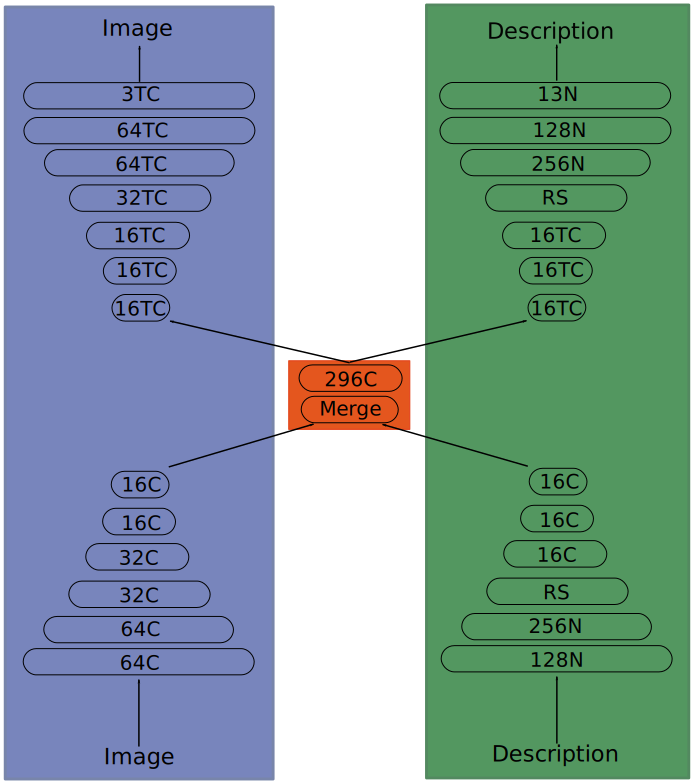
\includegraphics[width=0.75\textwidth]{Figs/shapes/maeArch.png}
\label{fig:final_arch}
\caption{\textcolor{red}{The architecture of the MAE used in \autoref{Chapter6} to generate the images seen in \autoref{fig:mrl_teaser}. Layers marked with C are convolution TC, Transposed Convolution, RS, Reshape and N, Dense.}}
\end{figure}

\textcolor{red}{\autoref{fig:final_arch} shows an overview of the \ac{MAE} architecture used in \autoref{Chapter6}. The \ac{MAE} used in \autoref{Chapter4} and \autoref{Chapter5} follow a very similar structure and are pictured later in \autoref{fig:netMnist} and \autoref{fig:netArts}.} 





%----------------------------------------------------------------------------------------







% Chapter Template

\chapter{Background} % Main chapter title

\label{Chapter2} % Change X to a consecutive number; for referencing this chapter elsewhere, use \ref{ChapterX}

\lhead{Chapter 2. \emph{Background}} % Change X to a consecutive number; this is for the header on each page - perhaps a shortened title

%----------------------------------------------------------------------------------------
%	SECTION 1
%----------------------------------------------------------------------------------------

\section{Introduction}\label{Lit:Intro}
In this section I will layout the key ideas and technologies which have inspired and enabled the research presented later in this thesis.

Due to the broad scope of the research carried out, the background section is loosely presented so as to compare and contrast the state-of-the-art artificial neural network technologies with their biological analogues (where possible). As such, I survey a large body of machine learning, psychology and biology literature.

In doing this, I aim to demonstrate how ANNs have exceeded human performance in specific areas, whilst lagging far behind in many others. By bringing these divergent fields together, perhaps it is possible to find ways to improve ANNs whilst also further developing our understanding of what makes humans tick. 


\section{What are Artifical Neural Networks good at?}
Artificial Neural Networks have been around for a long time but perhaps the best example of early neural networks is the MultiLayer Perceptron (MLP) \cite{rosenblatt1958perceptron}. Modern ANNs can trace their lineage back to the MLP, however the technology has advanced a lot since 1958. ANNs represent the state-of-the-art on many Artificial Intelligence benchmarks.

ANNs are currently enjoying a new renaissance due to wide spread availablity of Graphics Processing Units (GPUs), big data and software libraries like Tensorflow and CUDA.

In 2012, Krizhevsky et al. \cite{krizhevsky2012imagenet} kickstarted this new wave of interest in ANNs by getting the top performance on the ILSVRC-2012 ImageNet challenge. The unprecendented performance was achieved by utilising a very large amount of training data (1.2 million images), which was made possible by utilising the parallel computing power of GPUs. In creating AlexNet, Krizhevsky et al. demonstrated the potential of ANNs to solve real world problems, something which had been promised since ANN research began.

The field of Deep Learning (DL) has advanced greatly in recent years, with ANNs being used to solve many different types of problems. DL is being used for many differnt tasks. These can be broken down into several categories:


\begin{outline}
 \1 Classification:
   \2 Image Recognition \cite{krizhevsky2012imagenet, iandola2016squeezenet, he2016deep, zoph2018learning}
   \2 Speech Recognition \cite{amodei2016deep, graves2013speech}
   \2 Facial Recognition
   
 \1 Natural Language Processing:
    \2 Language Representation Learning \cite{mikolov2013distributed, mikolov2013efficient, mikolov2013linguistic}
 	\2 Intent Classification \cite{chen2016zero}
 	\2 Machine Translation \cite{cho2014learning}

 \1 Generation:
   \2 Image
   \2 Voice
   
 \1 Multimodal Learning:
 	\2 Image Captioning \cite{vinyals2015show}
 	\2 Video Captioning
 	\2 Multimodal Representation Learning \cite{ngiam2011multimodal}
   
 \1 Reinforcement Learning:
   \2 Robotic Control \cite{lillicrap2015continuous}
   \2 Video Games \cite{vinyals2019alphastar, mnih2013playing}
   \2 World Modelling \cite{azar2019world}
      
 \1 Forecasting:
   \2 Weather \cite{mahesh2018probabilistic}
   \2 Electrical Loads \cite{bouktif2018optimal}
   \2 Financial Markets \cite{fischer2018deep}
\end{outline}

\subsection{Classification}
\subsection{Generation}
\subsection{Representation Learning}
\subsection{Reinforcement Learning}


\section{What are Artificial Neural Networks bad at?}
Whilst ANNs have been applied to many tasks and acheived super-human ability at them \cite{vinyals2019alphastar}, they do not have general intelligence like humans.

\begin{displayquote}
``... people see how well [an algorithm] performs at one task and they think it can do all the things around that, and it can’t... When we see a person performing a task very well, we understand the competence [involved]. And I think they apply the same model to machine learning'' - Rodney Brooks.
\end{displayquote}
\subsection{Data Ineffciency}
look at oth ML methods which require less data but are generally less capable/require more engineering.


\section{How to get off the Symbol Grounding Merry-Go-Round} 
\subsection{What is symbol grounding?}
\subsection{How do humans do it?}
Barsalou

\subsection{How do machines do it?}

\section{Why brains are better}
\subsection{Embodiment}
\subsubsection{Sensory Redundancy}
\subsubsection{Biological Filters}
Retina, shape of ear etc.
\subsection{Development}
\subsubsection{Biological Filters, again}
Superior Colliculous guides learning in the visual cortex by controlling attention.
\subsection{Pulling yourself up by the bootstraps}

\subsection{Machine Equivelancy}
\subsubsection{How do we simulate Embodiment for ANNs?}
\subsubsection{How do we simulate Development for ANNs?}

\section{Where do we go from here?}
\subsection{Robot bodies}
\subsection{multimodality}
\subsection{transfer learning}



% Chapter Template

\chapter{Background} % Main chapter title

\label{Chapter3} % Change X to a consecutive number; for referencing this chapter elsewhere, use \ref{ChapterX}

\lhead{Chapter 3. \emph{Background}} % Change X to a consecutive number; this is for the header on each page - perhaps a shortened title

%----------------------------------------------------------------------------------------
%	SECTION 1
%----------------------------------------------------------------------------------------

\section{Introduction}\label{Lit:Intro}
In this section I will layout the key ideas and technologies which have inspired and enabled the research presented later in this thesis.

Due to the broad scope of the research carried out, the background section is loosely presented so as to compare and contrast the state-of-the-art artificial neural network technologies with their biological analogues (where possible). As such, I survey machine learning, psychology and biology literature.

In doing this, I aim to demonstrate how ANNs have very good performance in specific areas, whilst lagging far behind in many others. By bringing these divergent fields together, perhaps it is possible to find ways to improve ANNs whilst also further developing our understanding of what makes humans tick. 


\section{What are Artifical Neural Networks good at?}
Artificial Neural Networks have been around for a long time but perhaps the best example of early neural networks is the MultiLayer Perceptron (MLP) \cite{rosenblatt1958perceptron}. Modern ANNs can trace their lineage back to the MLP; however the technology has advanced a lot since 1958. ANNs represent the state-of-the-art on many Artificial Intelligence benchmarks.

ANNs are currently enjoying a new renaissance due to wide spread availablity of \ac{GPU}, big data and software libraries like Tensorflow and CUDA.

In 2012, Krizhevsky et al. \cite{krizhevsky2012imagenet} kickstarted this new wave of interest in \ac{ANN}s by getting the top performance on the ILSVRC-2012 ImageNet challenge. The unprecendented performance was achieved by utilising a very large amount of training data (1.2 million images), which was made possible by utilising the parallel computing power of \ac{GPU}s. In creating AlexNet, Krizhevsky et al. demonstrated the potential of \ac{ANN}s to solve real world problems, something which had been promised since \ac{ANN} research began.

The field of \ac{DL} has advanced greatly in recent years, with \ac{ANN}s being used to solve many different types of problems. DL is being used for many differnt tasks which can be broken down into several categories: Classification, \ac{NLP}, Data Generation, Reinforcement Learning and Prediction Tasks.


%\begin{outline}
% \1 Classification:
%   \2 Image Recognition \cite{krizhevsky2012imagenet, iandola2016squeezenet, he2016deep, zoph2018learning}
%   \2 Speech Recognition \cite{amodei2016deep, graves2013speech}
%   \2 Facial Recognition
%   
% \1 Natural Language Processing:
%    \2 Language Representation Learning \cite{mikolov2013distributed, mikolov2013efficient, mikolov2013linguistic}
% 	\2 Intent Classification \cite{chen2016zero}
% 	\2 Machine Translation \cite{cho2014learning}
%
% \1 Generation:
%   \2 Image
%   \2 Voice
%   
% \1 Multimodal Learning:
% 	\2 Image Captioning \cite{vinyals2015show}
% 	\2 Video Captioning
% 	\2 Multimodal Representation Learning \cite{ngiam2011multimodal}
%   
% \1 Reinforcement Learning:
%   \2 Robotic Control \cite{lillicrap2015continuous}
%   \2 Video Games \cite{vinyals2019alphastar, mnih2013playing}
%   \2 World Modelling \cite{azar2019world}
%      
% \1 Forecasting:
%   \2 Weather \cite{mahesh2018probabilistic}
%   \2 Electrical Loads \cite{bouktif2018optimal}
%   \2 Financial Markets \cite{fischer2018deep}
%\end{outline}

Of these categories of problems, \ac{MRL}(as it is presented in this thesis) draws mostly from Classification, \ac{NLP} and Data Generation, so these will be the focus of this survey.

\subsection{Classification}
\ac{MRL} can be considered to draw from different classification tasks, depending on which modalities it is used with. In this thesis I apply \ac{MRL} to image, speech and textual data, as such I will focus on general recognition techniques from the image processing domain and will not focus on more nitch problems such as Facial Recognition \cite{ma2004facial}, Emotion Recognition \cite{levi2015emotion} or more general data classification problems \cite{kussul2017deep,qi2017pointnet}.

\subsubsection{AlexNet}
With Krizhevsky's work in\cite{krizhevsky2012imagenet}, a style of \ac{ConvNet} architecture, consisting of convolution max-pooling and dropout layers followed by fully connected layers and a softmax output layer was created. This has become a standard type architecture for image classification tasks with many similar networks appearing such as VGG 16 and 19 \cite{simonyan2014very}.

Convolution layers are used for feature extraction and fully connected layers are used for classification with downsampling happening gradually throughout the network to reduce the dimensionality of the data. In AlexNet and VGG downsampling is done using the max-pooling layers, however more recent architectures have made use of strided convolutions for this \cite{springenberg2014striving}.

The use of dropout as a regulariser has also become common place as it has been shown to outperform the most common regularisers, L1 and L2 \cite{srivastava2014dropout}.

\subsubsection{Residual Connections}
An important advancement over the AlexNet style of architecture (beyond simply altering network hyper parameters as with VGG 16 and 19 \cite{simonyan2014very} was the addition of residual connections. Introduced in \cite{he2016deep}, residual connections allow data to flow through alternate branches of a network, skipping over some layers to rejoin the main flow at a later point in the network. This has two key effects, 1) it allows the training of much deeper networks by providing a shortcut through the network for error gradients to be backpropogated, helping to ellivate the vanishing gradient problem \cite{hochreiter1998vanishing} and 2) it allows the network to consider lower level features along side more abstracted ones for decision making.
An example of taking residual connections to their limit is seen in \cite{huang2017densely} where every preceeding layer's output is an input to the layers which follow it. This makes the neural network very wide but allows for good performance even with a small number of layers, offering a reduction in computational complexity.

\subsubsection{Inception: Multiscale Convolutions}
Another advancement over the AlexNet style architectures was the introduction of multiscale convolutions where data is passed through multiple, parallel convolutions layers each with a different kernel size before concatenating their activations \cite{szegedy2015going}. Making use of different kernel sizes creates filters which are sensitive to different scales of features. Thus, for example, if an eye in an image is not picked up at one scale as it is too large or too small, it may be picked up by a parallel convolution with a different sized kernel.

Szegedy et.al have developed their Inception Architecture from \cite{szegedy2015going} iteratively in \cite{szegedy2016rethinking, szegedy2017inception} in each, small advancements in state-of-the-art object recognition are achieved.


\subsection{Generation}
Whilst classification tasks are concerned with grouping input data into classes, generative tasks aim to create examples of particular classes, as with class conditioned \ac{GAN} \cite{mirza2014conditional, odena2017conditional} or to generate a translation from one modaility to another, for example image and video caption generation \cite{vinyals2015show, lebret2015phrase, donahue2015long, jia2015guiding, rohrbach2014coherent, rohrbach2013translating, yao2015describing, yao2015video, venugopalan2014translating, johnson2016densecap, ordonez2011im2text} and image style transfer \cite{zhu2017unpaired}.

We can also consider \ac{AE} a type of generative network due to the way in which they are trained, however, it is more useful to consider them from the perspective of representation learning. For example in \cite{lu2013speech} \ac{AE}s are used to generate denoised speech.

\subsubsection{Generative Adversarial Networks}
I will not spend much time on the \ac{GAN} based methods as they are not utilised in the research presented in this thesis. However, \ac{GAN}s are a very active area of research so here is a brief overview. 

In \cite{mirza2014conditional} the Generator network is fed noise and a class label is used to generate images of examples of that class. The Discriminator is fed the desired class and either a real or generated image and tasked with distinguishing whether the image is real or not. By inverting and backpropogating the error gradients from the Discriminator through the Generator, the Generator learns to fool the Discriminator by generating realistic images for each class in the dataset.

Odena et al. \cite{odena2017conditional} expand on the work in \cite{mirza2014conditional}. In stead of feeding the desired class to the Descriminator, they train an auxillory classifier network which classifies which class the generated and real images belong to.

GANs can also be used for style transfer \cite{zhu2017unpaired}. Style transfer is similar to translating from one modality to another, thus \cite{zhu2017unpaired} demonstrates the flexibility and power of \ac{GAN}s which could be applied to a much wider variety of problems than those I have highlighted here. Zhu et al. use the Descriminator of a \ac{GAN} to determine whether an image is from a given domain (e.g. Monet paintings) or was translated by the Generator from another domain (e.g. photos). In doing so the Generator learns to produce iamges in the chosen domain from images in a source domain (e.g. photo --> Monet painting).

\subsubsection{Modality Translation: Image Caption Generation}
Translating from one modality to another can also be done by other types of neural networks, not just those trained in an adversarial manner as with \ac{GAN}s.
The field of image and video captioning highlights this. The typical method for image caption generation is to first train a ConvNet on an image classification task and a language model (e.g. an \ac{LSTM} \cite{hochreiter1997long}) on a word prediction task \cite{vinyals2015show, venugopalan2014translating, johnson2016densecap}. This initalises the two subnetwroks to have useful weights for the task. In \cite{johnson2016densecap} Johnson et al. make use of the VGG net from\cite{simonyan2014very}. This off the shelf reuse of networks can be very useful and is explored in detail in \cite{keller}.
The dense layers of the \ac{ConvNet} are removed and the internal image representation learnt by the \ac{ConvNet} is fed to the language model which is then trained to predict image captions from this representation.

Video captioning is a natural extension of the iamge captioning domain and follows a similar procedure for generating video captions. First a representation of the visual contents of the video is generated and then a language model translates this representation into a caption. In order to generate a representation of the visual information  present in the videos, one can either make use of \ac{LSTM}s to combine the representations of each frame generated by a \ac{ConvNet} \cite{donahue2015long}, make use of 3D \ac{ConvNet}s, convolving along the time axis as well as the two spatial axes of the image frames \cite{yao2015describing, yao2015video} or make use of precomputed features such as Motion Boundary Histograms or Optical Flow \cite{rohrbach2014coherent, rohrbach2013translating}.

In all of these methods we see an important commonality, Representation Generation. In order to generate one modality from another, first a representation of the salient information from the source modality must be produced.

\subsection{Representation Learning}

Whilst many tasks involving \ac{ANN}s focus on an end result such as a \cite{krizhevsky2012imagenet}, others actively focus on learning data representations \cite{radford2015unsupervised, silberer2014learning, wavenet, vincent2010stacked, mikolov2013distributed, mikolov2013efficient, mikolov2013linguistic, feng2010visual, eslami2018neural, donahue2019large}.

Designing the manner in which data is represented is a vital part of building any machine learning system. As Bengio et al. note in \cite{repRev}:

\begin{displayquote}
``...much of the actual effort in deploying machine learning algorithms goes into the design of... data transformations that result in representations... that support effective machine learning.''
\end{displayquote}

As I discussed previously, image and video captioning are relient on learning abstract representations of the input images. In fact, representation learning is present in all neural network tasks, whether they are directly viewed this way or not. In \cite{vinyals2015show, venugopalan2014translating, johnson2016densecap}, not only is pretraining to produce a useful representation of image content leveraged, but we also see that learning this representation is inherent in learning image classification, highlighted by Johnson et al. \cite{johnson2016densecap} reusing weights trained in \cite{simonyan2014very}. 

\subsubsection{Natural Language Processing}
In \cite{mikolov2013distributed, mikolov2013efficient, mikolov2013linguistic} Mikolov et al. show how learning a continuous representation of natural language can be used to solve various \ac{NLP} tasks. By converting from a one-hot representation to a continuous representation, learnt through a word prediction task, many other problems can be solved. 
Whilst a one-hot encoding contains no information about the meaning of the word it represents, the continuous representation which arises from learning skip-gram or n-gram models which take this one-hot encoding as input do contain some of the meaning of the words they represent. This can be related to the Manifolds, Natural Clustering, and Temporal and Spatial Coherence properties which Bengio et al. \cite{repRev} put forward as being important parts of a good representation.

Whilst the skip-gram and n-gram representations remain ungrounded and do not contain the true meaning of the words they encode, some properties of the words can be found from this representation. For example, pronouns all end up with similar representations, showing the representation has Manifolds which are formed through Natural Clustering. This is also true for capital cities of countires. 

Further to this, the gradients between the representations of countries and their capitals are also similar. This highlights that some of the meaning of words can be found just from statistical regularities in bodies of text and to demonstrate that the representation exihibtis Spatial Coherence.


\subsubsection{Autoencoders}
\ac{AE}s are a very powerful class of networks which can be used for learning dense representations of many forms of data in an unsupervised manner.

\ac{AE}s learn a representation of the data they process by compressing the data into a smaller representation as explained in the \ref{Chapter2}.

In \cite{pu2016variational} Pu et al. make use of \ac{VAE}s to learn a representation of images, the image is then classified using a multiclass \ac{SVM} conditioned on the image representations from the \ac{VAE}. They compare their classification performance on various benchmarks demonstrating similar performance to state-of-the-art techniques but with much lower computation time. The computational performance gain is achieved due to a combination of using \ac{GPU}s and the reduction in computational complexity from the compression ofthe image data via the \ac{VAE}.

Pu et al. then replace the multiclass \ac{SVM} with a \ac{RNN} and training on an image captioning dataset (MS COCO\cite{lin2014microsoft}), learn to predict a series of one-hot encoded words, representing an image caption. On this task, the show better performance for caption generation using image representations generated by their \ac{VAE} than the representations generated by either VGG \cite{simonyan2014very} or the InceptionNet \cite{szegedy2015going}. They do not offer an explanation as to why the representation learned by their \ac{VAE} is better for this task than those learned by the classification task in \cite{simonyan2014very, szegedy2015going}; however, I will.
In \cite{repRev} Bengio et al. introduced a series of properties which a good representation should have. From these, two are particularly relevant to explaining the improved performance of the \ac{VAE} representation over the classifier based representations.

\begin{itemize}
	\item Semi-supervised learning: Given an input X and target Y a subset of the concepts explaing X's distribution explain much of Y given X.
	\item A hierarchical organisation of explanatory factors: The concepts that are useful for describing Y can be defined in a hierarchy of concepts with more abstract (high-level) concepts defined in terms of less abstract (low-level) ones.
\end{itemize}

Both the classification and \ac{VAE} based representations have both of these properties. However, when learning a representation for a classification task, the \ac{ANN} will focus on representing only the features useful for the classification. For example, if trying to learn to classify horses, it is the shape of the horse that matters not its colour (horses come in many colours, but whether a horse is brown, white or even blue does not change the fact that it is a horse). This means that whilst the classification representation contains low-level concepts for describing the shape of the horse, they do not contain low-level features for describing the high-level concepts of colour.
When captioning images of horses, the colour is very important as one would expect the caption to contain information about the horse beyond just that there is a horse. If the classification \ac{ANN} has thrown away the information about the colour of the horse, this information cannot appear in the caption. As the classification reprepresentation does not contain the concepts of colour, it does not have the the full subset of factors which describe Y given X if Y is the horse colour and X the image of the horse.

Consider now what the \ac{VAE} is trained to do, it learns to produce a compressed representation of the image from which the image can be reconstructed. This means that more of the information of the original image needs to be contained in the representation and is therefore available for generating accurate captions of that image. I.e. the full subset of concepts which describe Y given X are available, meaning the \ac{VAE} representation fullfils both the semi-supervised learning and hierarchical organisation of explanitory factors to a greater degree than the classification representation.

In a second experiment, Pu et al. train their caption generation system in an end-to-end fashion, this lead to a significant improvement in performance (+0.11 BLEU \cite{bleu}). This demonstrates that the representation of the \ac{VAE} can be improved upon by adapting the feature extraction process specifically for the captioning task.


As well as representations of images, \ac{AE} can be used to learn representations of other types of data. A good example of this is WaveNet \cite{wavenet}. Chorowski et al. demonstrate how strided convolutions \cite{radford2015unsupervised} can be used to capture the time dependant regularites of speech at different scales within an vector quantised autoencoding architecture \cite{van2017neural}. Chorowski et al. build off of a large body of research on speech representation using \ac{AE}s \cite{vincent2010stacked, lu2013speech}.

The WaveNet architecture stacks layers of strided convolutions with each successive layer having a larger stride, this allows the network to consider features from more and more distant (in time) points of the input data. An intuitive way of understanding why this is useful for generating a representation of speech is to imagine two different speakers saything the same word. One speaker speaks very quickly and the other very slowly. This means that the same word, said by each speaker will have different characteristics with respect to time but as each speaker is saying the same word, the network must be able to ignore this variation with respect to time.

Chorowski show that their unsupervised, speaker independant WaveNet is able to beat the state-of-the-art performance on a phonetic unit discovery task \cite{dunbar2017zero} on two out of three languages (English and French) demonstrating that the WaveNet representation can be used to correctly distinguish between phonemes. The languages it acheived the best results for had significantly more training data, though for the third language (Mandarin) it achieved comparable results to other entrants to the ZeroSpeech 2017 challenge. 

What is of particular interest in \cite{wavenet} is that it achieves state-of-the-art performance on this challenge in an unsupervised manner. The authors note that it is better to have a model which requires and is capable of exploiting the large amount of unlabelled data through unsupervised training, than to have a simpler model which saturates on small datasets. The authors suggest that this is one reason why WaveNet did not achieve state-of-the-art performance on Mandarin due to overfitting the small amount of training data.

They also note that Mandarin is a pitched language, unlike English and French, and that the WaveNet disgards pitch and prosody \cite{van2017neural} which may be important features for distinguishing Mandarin Phonemes. As the authors do not test whether the addition of more unsupervised training improves the representation of Mandarin phonemes, it is unclear whether the WaveNet architecture is the right choice for generating representations of Mandarin. In my opinion, the use of vector quantisation to make the latent space discrete, whilst helping to prevent a collapse in the latent space, discards too much useful information as shown by the superior performance of the \ac{VAE}, which uses a continuous latent representation, at representing pitch information \cite{wavenet}. 

\section{What are Artificial Neural Networks Bad at?}
Whilst ANNs have been applied to many tasks and acheived super-human ability at them \cite{vinyals2019alphastar}, they do not have general intelligence like humans.

\begin{displayquote}
``... people see how well [an algorithm] performs at one task and they think it can do all the things around that, and it can’t... When we see a person performing a task very well, we understand the competence [involved]. And I think they apply the same model to machine learning'' - Rodney Brooks.
\end{displayquote}

\subsection{Artificial Neural Networks are Easily Fooled}
Whilst \cite{krizhevsky2012imagenet, simonyan2014very, szegedy2015going, szegedy2016rethinking, szegedy2017inception, he2016deep, huang2017densely, russakovsky2015imagenet, chiu2018state, eslami2018neural} all show amazing performance on a very difficult image classification problem. These same networks are easily fooled by images, which to humans look like random noise \cite{nguyen2015deep}.

\todo[inline]{Discuss more \cite{nguyen2015deep} plus other citations, papers are on desk at work}

\subsection{Data Ineffciency}
As demonstrated by WaveNet's poor performance at representing Mandarin speech \cite{wavenet} when \ac{ANN}s are not provided with enough data they often overfit and fail to distinguish between salient features and local noise in the training data. A large portion of the success of AlexNet \cite{krizhevsky2012imagenet} is due to the 1.2 million images that were used to train it. This was only possible due to the advancement of \ac{GPU} technology allowing for parallel computation of each convolution in the network. Attempting to train AlexNet on a \ac{CPU} would take a very long time.

Similarly, Vinyals et al. \cite{vinyals2015show} report that their image captioning system required millions of training instances to achieve their then state-of-the-art performance, even after pretraining on the 1.2 million images from ImageNet \cite{ImNet}.

Ha et al. \cite{ha2018world, ha2018recurrent} do show that pretraining pretraining an unsupervised world representation can allow for rapidly producing controllers capable of solving reinforcement learning tasks. However this is not generalisable to all problem spaces.

Obviously, \ac{ANN}s are not comparable to adult humans when it comes to learning complex, high level tasks with little or no training. It is expected that an adult human could recognise a novel object and its name from a single training example, this is not to be expected from an \ac{ANN}.

Ha's approach of producing a compressed and feature rich representation of the world \cite{ha2018world, ha2018recurrent} may offer insight into how we can approach human like performance at one-shot-learning \cite{vinyals2016matching}. As demonstrated in the representation learning literature, pre-learning a representation which fulfils the criteria layed out in \cite{repRev} can greatly simplify many machine learning tasks.


\section{How to get off the Symbol Grounding Merry-Go-Round} 
\subsection{What is symbol grounding?}
\cite{searle1980minds, steels2008symbol}
\subsection{How do humans do it?}
\cite{barsalou2008grounded}

\subsection{How do machines do it?}
\cite{coradeschi2000anchoring, coradeschi2003introduction, pezzulo2013computational, cangelosi2001adaptive, cangelosi2002symbol}

\todo[inline]{this has just been shoved in here and will need to be rewritten}
In \cite{ngiam2011multimodal}, a MAE was trained using video and pre-processed audio data to classify speech data. They demonstrate that the addition of the visual data improves recognition under noisy conditions, highlighting the technical advantages of MAEs. Further to this they demonstrate that the McGurk effect \cite{mcgurk1976hearing} occurs in the MAE, highlighting that it is a good analogy for the human audio and visual cortices and how they interact.

In \cite{silberer2014learning}, Silberer et al. demonstrate the ability of MAEs to reconstruct missing data when only one modality is present. A similar effect is seen in the human brain where sensory redundancy is utilised to repair and reconstruct data from noisy or missing percepts \cite{samuel1997lexical}. We use this effect to reconstruct images from audio. 

\section{Why brains are better}
\subsection{Embodiment}
\cite{pfeifer2006body, smith2005development}
\subsubsection{Sensory Redundancy}
\subsubsection{Biological Filters}
Retina, shape of ear etc.
\subsection{Development}
\subsubsection{Biological Filters, again}
In \cite{johnson2015two}, Johnson et al. comment on the well established `two process theory of face processing' in humans.  During the `Conspec' stage of the \ac{TPT} the superior colliculus interacts with both visual and motor systems driving visual attention towards conspecific stimuli. The `Conlern' stage of the \ac{TPT} is guided by the `Conspec' stage due to a larger proportion of conspecific visual data  (e.g. the human face) being provided to the visual cortex as more attention is given to these stimuli by the superior colliculus. 
The Superior Colliculous guides learning in the visual cortex by controlling attention.

Bambach \cite{bambach2017egocentric} highlights the importance of data quality when training visual recognition systems, thus the superior colliculus may help to improve the learning of the visual cortex by providing focused, high-quality training examples.

As well as the structure of the human brain which has been optimised by evolution to facilitate rapid learning, the physical embodiment of humans guides and improves human learning. Possibly the best example of this is the human eye, specifically the retina.

The highly organised nature of the retina predisposes the types of visual data presented to the visual cortex to have certain characteristics through signal conditioning, as well as shape and movement specific sensitivity \cite{masland2012neuronal}.

Signal conditioning in the retina enhances object boundary detection by reducing the brightness of the brightest areas and their immediate surroundings, giving objects a rough outline. Other effects in the retina are sensitive to movement and help segment the background from moving objects in the foreground \cite{olveczky2003segregation}.

Similarly, the shape of the human ear and the physical structure of the inner ear filters and shapes the sounds we hear which facilitates learning and detection of relevant sounds whilst reducing the perception of background noise \cite{oxenham2018we}.
\subsection{Pulling yourself up by the bootstraps}

\subsection{Machine Equivelancy}
\subsubsection{How do we simulate Embodiment for ANNs?}
\cite{lee2008sparse}
\subsubsection{How do we simulate Development for ANNs?}

\section{Where do we go from here?}
\subsection{Robot bodies}
\subsection{multimodality}
\subsection{transfer learning}


 
 
% Chapter Template

\chapter{Sensory Redundancy: Are two heads better than one?} % Main chapter title

\label{Chapter4} % Change X to a consecutive number; for referencing this chapter elsewhere, use \ref{ChapterX}

\lhead{Chapter 4. \emph{Sensory Redundancy: Are two heads better than one?}} % Change X to a consecutive number; this is for the header on each page - perhaps a shortened title

%----------------------------------------------------------------------------------------
%	SECTION 1
%----------------------------------------------------------------------------------------

\section{Why have one sensor when two are better?}
A key part of the human experience is that it is multisensory. In \cite{barsalou2008grounded}, Lawrence Barsalou speaks about how multisensory processing aids human cognition in a number of ways. Firstly, multisensory information aids in the classification of experiences by providing additional and complimentary information that is not accounted for in only a single modality. 

The Mcgurk effect \cite{mcgurk1976hearing} demonstrates how the visual stimuli of lip reading affects the classification of heard sounds. Whilst this effect can lead to incorrect classifications when misaligned data is provided e.g. utterances of the syllable [ba] dubbed on to lip movements for [ga], lead to normal adults hearing [da]; in normal circumstances, like when two people are speaking to one and other, lip reading aids in classifying heard sounds \cite{ma2009lip}. This is particularly important in noisy environments, which leads to another of Barsalou's ideas about multisensory processing: information redundancy.

The reason that lip reading can aid hearing in noisy evironments is that it provides an additional vector along which the human brain can reconstruct missing information. When something is mis-heard due to background noise, the visual information gained from looking at the face of the speaker can be used to reconstruct their utterance.

The ability to reconstruct missing data from a secondary modality has not only been seen in humans \cite{ma2009lip, samuel1997lexical} but has been demonstrated in computational modals for example, Ngiam et al.\cite{ngiam2011multimodal}.

In order to be able to reconstruct missing data from a secondary modality, symbol grounding needs to have occured, and the meaning of a percept in modality A must be known in modality B.
If both the forward and inverse relationship between modalities is known, then bidirectional symbol grounding has occured and we are able to reconstruct modality A from modality B and modality B from modality A.

In this chapter I will explore these two ideas, improved classification and reconstruction of missing information through  bidirectional symbol grounding using multimodal autoencoders (MAE).



\section{Generating images from natural language}
\subsection{Aims}
The experiment in this section demonstrates that having access to a second modality improves classification accuracy over the baseline accuracy of classification of either of the two individual modalities as well as how missing data can be reconstructed from a secondary modality.

\subsection{UCU Arabic Spoken Digits and MNIST} 
\label{sec:UCU}
This experiment utilises two datasets, UCU Arabic Spoken Digits (UCU) and MNIST Handwritten Digits (MNIST).

\subsubsection{UCU Arabic Spoken Digits}
UCU is a dataset containing the 13 Mel Frequency Cepstrum Coefficients representing the audio of the digits 0 to 9 being said by 88 different speakers \cite{hammami2009tree,hammami2010improved}. It contains 8800 utterances (10 digits x 10 repetitions x 88 speakers). Audio was sampled at 11025Hz.

\paragraph{Padding of Utterances}
As utterances are not of a fixed length, it is necessary to pad the utterances to be equal length. The longest utterance in the dataset contains 93 samples. For ease of up and downsampling within the neural network, all uttereances are padded to be 100 samples long by appending zeros. Each sample is also padded to contain 16 features, the 13 MFCCs and 3 zeros to further facilitate up and down sampling\footnote{Up and down sampling is easier with even numbers of features and samples as we can half the size of the data using strided convolutions, s=(2,2), without worrying about integer division errors e.g. $5/2=2$ but $2\times2 \neq5$}.

As I will be classifying the digits, it is necessary to check that padding the digits does not provide a cheat for this. As such, I analise the mean number of samples for each digit and their standard deviations as depicted in \autoref{fig:ucu_dig_length}. I then perform a linear regression on the number of samples to demonstrate that it is not possible to accurately predict a digits class given only the length of the utterance.

\begin{figure}
\centering
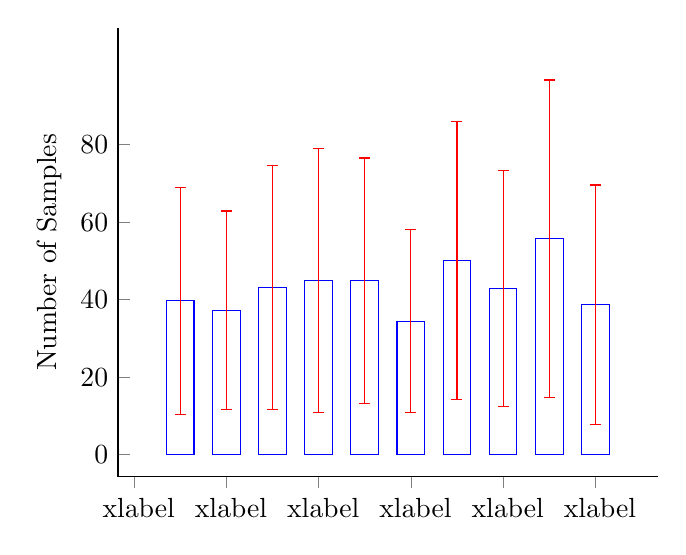
\begin{tikzpicture}
\begin{axis}[
	axis x line*=bottom,
	axis y line*=left,
	%at={(-1,0)}
    ybar,
    enlargelimits=0.15,
    ylabel={Number  of Samples},
    ytick={0,20,40,60,80},   
    xtick={},
    xticklabel={} %{zero, one, two, three, four, five, six, seven, eight, nine}
    %x tick label style={rotate=45},
    xlabel={Digit},
    %nodes near coords,
    %nodes near coords align={vertical},
    xlabel near ticks,
	ylabel near ticks,
	bar shift=0pt
    ]
%\addplot coordinates {(1,39.66) (2,37.27) (3,43.11) (4,45.02) (5,44.92) (6,34.44) (7,50.10) (8,42.81) (9,55.67) (10,38.63)};
\addplot[blue, error bars, y dir=both,y explicit, error bar style={color=red}]
 coordinates { 
(1,39.66) +- (0.0,29.25) 
(2,37.27) +- (0.0,25.58) 
(3,43.11) +- (0.0,31.43) 
(4,45.02) +- (0.0,34.05) 
(5,44.92) +- (0.0,31.63) 
(6,34.44) +- (0.0,23.63)
(7,50.10) +- (0.0,35.90)
(8,42.81) +- (0.0,30.41)
(9,55.67) +- (0.0,41.01)
(10,38.63) +- (0.0,30.94)
  };
\end{axis}
\end{tikzpicture}

	%\includegraphics[width=\textwidth]{./Figs/mnistSpoken/UCU_digit_length.png}
	\caption{Mean number of samples for each digit in the UCU Arabic Spoken Digits Dataset. Red bars show the standard devaition in length for each each digit.}
	\label{fig:ucu_dig_length}

\end{figure}

\autoref{fig:ucu_dig_length} shows the mean number of samples for each digit in the UCU dataset. Whilst there is a difference in the mean length of each digit, the standard deviation for each digit is relatively large as can be seen in \autoref{tab:UCU_sampLen}. Therefore, trying to classifiy the digits just by the number of samples in an example, is ineffective.

	\begin{table}
		\centering
		\begin{tabular}{|c|c|c|}
			\hline
			Digit & Mean Length (samples) & Standard Deviation \\ \hline
			0 & 39.66 & $\mypm 29.25$ \\ \hline
			1 & 37.27 & $\mypm 25.58$ \\ \hline
			2 & 43.11 & $\mypm 31.43$ \\ \hline
			3 & 45.02 & $\mypm 34.05$ \\ \hline
			4 & 44.92 & $\mypm 31.63$ \\ \hline
			5 & 34.44 & $\mypm 23.63$ \\ \hline
			6 & 50.10 & $\mypm 35.90$ \\ \hline
			7 & 42.81 & $\mypm 30.41$ \\ \hline
			8 & 55.67 & $\mypm 41.01$ \\ \hline
			9 & 38.63 & $\mypm 30.94$ \\ \hline

		\end{tabular}
		\caption{Mean length and standard deviation of digits in the UCU dataset.}
		\label{tab:UCU_sampLen}
	\end{table}


Performing a linear regression on the number of samples for each digit versus its class, we get an accuracy of 6.18\% when classifying the test set.

\subsubsection{MNIST Handwritten Digits}
MNIST is a well known and ofte used dataset in the machine learning community. It contains 60000 training samples and 10000 test samples, evenly split between the digits 0 to 9. 
Each digit is presented as a grey-scale, 28x28 pixel image \cite{lecun1998mnist}. 

\subsection{Problem Description}
The experiments with these datasets will explore two problems, classification and bidirectional symbol grounding. 

\subsubsection{Classification}
Each of the utterances and images from the UCU and MNIST datasets are classified as being a numeric digit, 0 to 9. By combining both datasets, we can explore whether the addition of a second modality enhances overall classification accuracy.

I start off exploring the classification abilities of neural networks by performing a linear regression with a single, dense neural network layer with a softmax activation on the activation of the embedding layer of an autoencoder. To generate baseline classifications accuracies for each dataset, I use autoencoders for each modality separately.

Once a classification baseline has been established for each dataset, I make use of a MAE, using paired examples from each dataset to train it.

\subsubsection{Bidirectional Symbol Grounding}

I demonstrate that a neural network can perform bidirectional symbol grounding \cite{barsalou2008grounded} when presented with aligned images and utterances. To explore this, I show how a MAE can learn to reconstruct the correct image of a digit given the MFCCs of an utterance as well as MFCCs which have a small mean squared error from the correct utterance given an image of a digit. This shows that an internal symbolic language has been learnt in the form of the latent embedding created by the encoders of the MAE.


\subsection{Experiment Details}
Images from the MNIST dataset are kept at their original scale of 28x28 pixels and are normalised such that each pixel has a value from 0 to 1 based on it's intensity, with zero equating to black and 1 being white.

The UCU dataset is normalised so that all MFCCs take a value from 0 to 1 based on the value of the MFCC such that the highest value is 1 and the lowest 0. Utterances are padded to be 100x16 as previously described.

\paragraph{Combining Datasets}
\label{sec:UCU_mnist_comb}
Due to the difference in size between the datasets, 8,800 samples for UCU and 80,000 samples for MNIST, I randomly sample from the UCU dataset and pair this with a sample from MNIST. This means that each sample from UCU is used approxiamtely 9.1 times ($80000/8800=9.0909$) in the training data.

\paragraph{Merging Modalities}
In order to combine the two different modalities, I explore different merging techniques: concatenation (\textit{Concat}) and addition (\textit{Add}). To do this, the embeddings of both modalities are ensured to have the same shape and then are merged using the methods described in \autoref{eqn:concat} and \autoref{eqn:add} for concatenation and addition, respectively. %and \ref{eqn:xply}.

 \begin{equation}\label{eqn:concat}
 	merged = Im_i^{emb} || MFCC_i^{emb} 	
 \end{equation}

 \begin{equation}\label{eqn:add}  
 	merged = Im_i^{emb} + MFCC_i^{emb} 	
 \end{equation}
 
  %\begin{equation}
 	%merged = x1^*_i * x2^*_i
 	%\label{eqn:xply}  
 %\end{equation}

Where $Im_i^{emb}$ and $MFCC_i^{emb}$ represent the embeddings, output by the image and MFCC encoders respectively for image and MFCC inputs $Im_i$ and $MFCC_i$.

\subsubsection{Training Procedures}

The MAEs are trained in two different ways for both types of merging, these are referred to as bimodal (Bi) and randomly degraded (RD).

\paragraph{Bimodal}
Under the Bi training procedure, the MAE is presented with bimodal input for all training instances. Both image and MFCC inputs are present for all training steps and the MAE is trained to reproduce this input as its output.

\paragraph{Randomly Degraded}
Under the RD training procedure, one third of image inputs are removed at random and a third of MFCC inputs are removed at random. It is ensured that each training instance always has at least one input modality present. That is, a training instance never has both its image and MFCC input removed. 

The removed modality is replaced with an array of zeros of the same shape as the original input (28x28 for the image and 100x16 for MFCCs).

The MAE is then trained to reproduce both the image and MFCCs regardless of whether one of these has been ommited from the input.

\subsubsection{Testing Conditions}
Each MAE (\textit{Concat} and \textit{Add}) was tested in three different ways, Bimodal, Image Only and MFCC Only.

\paragraph{Bimodal}
In the Bimodal testing condition both image and MFCC data are used as input for each testing instance and I am interested in observing the classification accuracy as well as the total regeneration error.

\paragraph{Image Only}
In the Image Only testing condition, only images are provided as input data. I am interested in the classification accuracy as well as the MFCC reconstruction error. I am not interested in the image reconstruction error, as it is expected that, as the image is provided as input this will be low (which it is for all models and training procedures as seen in \autoref{tab:mnist_ucu_master_res}).  

\paragraph{MFCC Only}
Similarly to the Image Only condition, the MFCC Only (MFCC) condition provides only MFCCs as input and I am interested in the classification accuracy as well as the image reconstruction error. I am not interested in the MFCC regeneration loss as MFCCs are given as input it will be low (which it is for all models and training procedures as seen in \autoref{tab:mnist_ucu_master_res}).  

\subsubsection{Network Description}
\paragraph{Baseline Models}
To generate the baseline classification accuracies for both the UCU and MNIST data, I make use of (unimodal) autoencoders. The descrition of the autoencoder for the MNIST dataset can be found in \autoref{tab:MNIST_AE_description} and the autoencoder for the UCU dataset in \autoref{tab:UCU_AE_description}.

	\begin{table}[h]
		\centering
		\begin{tabular}{|c|c|c|c|c|c|c|}
			\hline
			Block & Layer & Type & Neurons & Kernel & Strides & Activation  \\ \hline
			\multirow{4}{*}{Encoder} & 1	&	2D Conv & 32 & (3,3) & (1,1)  & Relu\\ \cline{2-7}
			& 2	&	2D Conv & 64 & (3,3) & (2,2) & Relu \\ \cline{2-7}
			& 3	&	2D Conv & 64 & (3,3) & (2,2) & Relu \\ \cline{2-7}
			& 4 	&	Dropout p=0.25 &	 & 	     &       & \\ \hline
			Embedding & 5	&	2D Conv & 32 & (3,3) & (1,1) & Relu \\ \hline
			Classifier & 6c	&	Dense          & 10 &       &       & Softmax      \\ \hline
			\multirow{5}{*}{Decoder}& 6 	&	Dropout p=0.25 &	 & 	     &       & \\ \cline{2-7}
			& 7	&	2D Trans Convn & 64 & (3,3) & (2,2) & TanH \\ \cline{2-7}
			& 8	&	2D Transp Conv & 64 & (3,3) & (2,2) & TanH \\ \cline{2-7}
			& 9	&	2D Trans Conv & 32 & (3,3) & (1,1) & TanH \\ \cline{2-7}
			& 10	&	2D Trans Conv & 1 & (3,3) & (1,1) & Sigmoid \\ \hline
		\end{tabular}
		\caption{Image autoencoder and classifier. Layer 6c performs classification, whilst the branch starting at layer 6 regenerates the image.}
		\label{tab:MNIST_AE_description}
	\end{table}

	\begin{table}[t]
		\centering
		\begin{tabular}{|c|c|c|c|c|c|c|}
			\hline
			Block & Layer & Type & Neurons & Kernel & Strides & Activation  \\ \hline
			\multirow{5}{*}{Encoder} & 1	&	2D Conv & 32 & (3,3) & (1,1)  & Relu\\ \cline{2-7}
			& 2	&	2D Conv & 64 & (3,3) & (2,2)  & Relu\\ \cline{2-7}
			& 3 	&	Dropout p=0.25 &	 & 	     &        & \\ \cline{2-7}
			& 4	&	Dense          & 3136 & 	 &        & \\ \cline{2-7}
			& 5   &	Reshape (7,7,64) &    &     &        & \\ \hline
			Embedding & 6	&	2D Conv & 32 & (3,3) & (1,1)  & Relu  \\ \hline
			Classifier & 7c	&	Dense          & 10 &       &        & Softmax \\ \hline
			\multirow{7}{*}{Decoder} & 7 	&	Dropout p=0.25 &	 & 	     &        & \\ \cline{2-7}
			& 9	&	Dense			& 3200 &     &        & \\ \cline{2-7}
			& 10	&	Reshape (25,4,32) &    &    &        & \\ \cline{2-7}
			& 11	&	2D Trans Conv & 64 & (3,3) & (2,2)  & TanH \\ \cline{2-7}
			& 12	&	2D Trans Conv & 64 & (3,3) & (2,2)  & TanH \\ \cline{2-7}
			& 13	&	2D Trans Conv & 32 & (3,3) & (1,1)  & TanH \\ \cline{2-7}
			& 14	&	2D Trans Conv & 1 & (3,3) & (1,1) & Sigmoid \\ \hline
		\end{tabular}
		\caption{MFCC autoencoder and classifier. Layer 7c performs classification, whilst the branch starting at layer 7 regenerates the MFCCs. The addition of reshape layers is to ensure the final shape of the regenerated MFCCs matches the target shape whilst the embedding shape matches that of the embedding of the image autoencoder.}
		\label{tab:UCU_AE_description}
	\end{table}

\paragraph{Multimodal Autoencoder}
By combining the two autoencoders described in \autoref{tab:MNIST_AE_description}, and \autoref{tab:UCU_AE_description}, a multimodal autoencoder is created. The embeddings from each of the unimodal autoencoders are merged by either, concatenation or addition.
 
	\begin{table}
		\centering
		\begin{tabular}{|c|c|c|c|c|c|c|}
			\hline
			Block & Layer & Type & Neurons & Kernel & Strides & Activation \\ \hline
			\multirow{2}{*}{Image} & 1i	&	2D Conv & 32 & (3,3) & (1,1) & Relu \\ \cline{2-7}
			& 2i	&	2D Conv & 64 & (3,3) & (2,2) & Relu \\ \cline{2-7}
			\multirow{2}{*}{Encoder}& 3i	&	2D Conv & 64 & (3,3) & (2,2) & Relu \\ \cline{2-7}
			& 4i	&	Dropout p=0.25 &	 & 	     &       &  \\ \hline

			\multirow{3}{*}{MFCC} & 1m	&	2D Conv & 32 & (3,3) & (1,1) & Relu \\ \cline{2-7}
			& 2m	&	2D Conv & 64 & (3,3) & (2,2) & Relu \\ \cline{2-7}
			& 3m 	&	Dropout p=0.25 &	 & 	     &       & \\ \cline{2-7}
			\multirow{2}{*}{Encoder} & 4m	&	Dense          & 3136 & 	 &       & \\ \cline{2-7}
			& 5m  &	Reshape (7,7,64) & & & & \\ \hline

			Merge & 6im	& Merge & & & & \\ \hline
			Embedding& 7im	&	2D Conv & 32 & (3,3) & (1,1) & Relu \\ \hline
			Classifier & 8c	&	Dense          & 10 &       &       & Softmax \\ \hline

			\multirow{3}{*}{Image} & 8i 	&	Dropout p=0.25 &	 & 	     &       & \\ \cline{2-7}
			& 9i	&	2D Trans Conv & 64 & (3,3) & (2,2)  & TanH \\ \cline{2-7}
			& 10i	&	2D Trans Conv & 64 & (3,3) & (2,2)  & TanH \\ \cline{2-7}
			\multirow{2}{*}{Decoder}& 11i	&	2D Trans Conv & 32 & (3,3) & (1,1)  & TanH \\ \cline{2-7}
			& 12i	&	2D Trans Conv & 3 & (3,3) & (1,1) & Sigmoid\\ \hline 

			\multirow{4}{*}{MFCC} & 8m 	&	Dropout p=0.25 &	 & 	     &        & \\ \cline{2-7}
			& 9m	&	Dense			& 3200 & &           & \\ \cline{2-7}
			& 10m	&	Reshape (25,4,32) & & & &\\ \cline{2-7}
			& 11m	&	2D Trans Conv & 64 & (3,3) & (2,2)  & TanH \\ \cline{2-7}
			\multirow{3}{*}{Decoder}& 12m	&	2D Trans Conv & 64 & (3,3) & (2,2)  & TanH \\ \cline{2-7}
			& 13m	&	2D Trans Conv & 32 & (3,3) & (1,1)  & TanH \\ \cline{2-7}
			& 14m	&	2D Trans Conv & 1 & (3,3) & (1,1)  & Sigmoid\\ \hline
		\end{tabular}
		\caption{Image and MFCC multimodal autoencoder. Layers marked i, m, im and c are image, MFCC, image and MFCC and classification respectively.}
		\label{tab:UCU_MNIST_MAE_description}

	\end{table}




\subsection{Results}

\subsubsection{Classification Results}
The complete set of results for this experiment are available in \autoref{tab:mnist_ucu_master_res} in \autoref{appendix:A}. The most important results are shown in the following three tables: \autoref{tab:mnist_ucu_bi_res} for the Bimodal testing condition, \autoref{tab:mnist_ucu_im_res} for the Image Only condition and \autoref{tab:mnist_ucu_mfcc_res} for the MFCC Only testing condition. 

All results reported here are the mean of a four-fold cross validation. Each training and testing condition was run four times and the average results are shown.


\begin{table}[h]
	\centering
		\begin{tabular}{|c|c|c|c|c|}
		\hline
		Model & Training & Im MSE & MFCC MSE &  Acc \\ \hline
				Image AE & Im & 	\textbf{0.0027}	&	       			& 	0.9883			\\ \hline		
				MFCC AE & MFCC & 		    		& 	\textbf{0.0113} &	0.9832			\\ \hline		
\multirow{2}{*}{Add MAE} & Bi & 	0.0030			&	0.0401			&	0.9967			\\ \cline{2-5}
						  & RD &	0.0033			&	0.0176			&	\textbf{0.9993}	\\ \hline	
		
\multirow{2}{*}{Concat MAE} & Bi & 0.0031			&	0.0423			&	0.9945			\\ \cline{2-5}		
							 & RD & 0.0030			&	0.0426			&	0.9986			\\ \hline
		\end{tabular}
		\caption{Mean Squared Errors for the Bimodal testing condition.}
		\label{tab:mnist_ucu_bi_res}

\end{table}

In \autoref{tab:mnist_ucu_bi_res} it can be seen that both concatenate and addition merging produce models with better prediction accuracy than the baseline models, regardless of training procedure.

\begin{table}
	\centering
		\begin{tabular}{|c|c|c|c|}
		\hline
		Model & Training &  MFCC MSE &  Acc \\ \hline
		Image AE & Im 		&  		    			& \textbf{0.9883}	\\ \hline		
\multirow{2}{*}{Add MAE} & Bi & 	0.1641			& 0.4501 			\\ \cline{2-4}
						  & RD & \textbf{0.0455}	& 0.9834 			\\ \hline	
		
\multirow{2}{*}{Concat MAE} & Bi & 	0.2029		&	0.3496 			\\ \cline{2-4}		
							 & RD & 	0.0737		&	0.9834 			\\ \hline
		\end{tabular}
		\caption{Mean Squared Errors for the Image Only testing condition.}
		\label{tab:mnist_ucu_im_res}

\end{table}

In comparison to the results shown in \autoref{tab:mnist_ucu_bi_res}, the results in \autoref{tab:mnist_ucu_im_res} show that the MAEs trained using the Bi training procedure do not generalise well when only a single input modality is available. Where as the MAEs trained using the RD training procedure perform almost as well as the baseline model. 
\begin{table}[h]
	\centering
		\begin{tabular}{|c|c|c|c|}
		\hline
		Model & Training & Im MSE &  Acc \\ \hline
				
				MFCC AE & MFCC & 					& 	\textbf{0.9832}	\\ \hline		
\multirow{2}{*}{Add MAE} & Bi & 	0.1138			& 	0.9624 			\\ \cline{2-4}
						  & RD &	0.0556			&	0.9789			\\ \hline	
		
\multirow{2}{*}{Concat MAE} & Bi &	0.1138			&	0.9455			\\ \cline{2-4}		
							 & RD & \textbf{0.0554}	& 	0.9827 			\\ \hline
		\end{tabular}
		\caption{Mean Squared Errors for the MFCC Only testing condition.}
		\label{tab:mnist_ucu_mfcc_res}

\end{table}

Similarly, the reuslts in \autoref{tab:mnist_ucu_mfcc_res} show that the behaviour of the MAEs is very similar under the RD training procedure regardless of whether it is MFCCs or images provided as input. However, the classification accuracy remains reasonably good under the Bi training procedure when only MFCCs are present. 

\subsubsection{Reconstruction Results}

In \autoref{fig:mnistDigits} examples of reconstructed digits generated by both the \textit{Add} and \textit{Concat} MAEs are shown.

\begin{figure}[h]
\begin{center}
	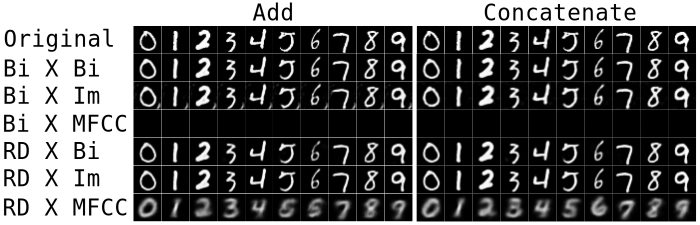
\includegraphics[width=\textwidth]{Figs/mnistSpoken/lbAll.png}
	\caption{A selection of randomly sampled digits generated in different training and testing conditions for both \textit{Add} and \textit{Concat} merging methods.}
	\label{fig:mnistDigits}
\end{center}
\end{figure}

\autoref{fig:5s} shows a comparison of two different examples of the digit ``5''. One is (subjectively) poorly written and the other is more prototypical and well formed. Under different testing conditions, the MAEs regenerate different ``fives''.

\begin{figure}[h]
\begin{center}
	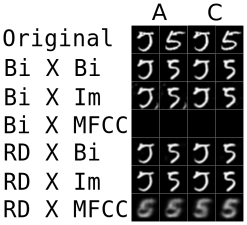
\includegraphics{Figs/mnistSpoken/5s.png}
	\caption{Two examples of the digit ``5'' being generated in different training and testing conditions for both \textit{Add} and \textit{Concat} merging methods.}
	\label{fig:5s}
\end{center}
\end{figure}



\subsection{Discussion}

\subsubsection{Discussion of Classification Results}
\autoref{tab:mnist_ucu_bi_res} shows that both the \textit{Add} and \textit{Concat} MAEs have better classification accuracy than the baseline, unimodal models. However, it is not clear that there is a difference in between the two training procedures, Bi and RD.

The difference between the two training procedures becomes clear in \autoref{tab:mnist_ucu_im_res} where it can be seen that the MAEs trained using the Bi training procedure have much worse classification rates when presented with only images as input. Models perform less than half as well as the baseline model, 0.4501 (\textit{Add}) and 0.3496(\textbf{Concat}) versus 0.9832 for the baseline image autoencoder.

There is a trade off between unimodal accuracy and mulitmodal accuracy in the RD training procedure MAEs. Whilst both the \textit{Add} and \textit{Concat} MAEs outperform the baseline models in the Bimodal test condition, they have slightly worse performance when tested with either images or MFCCs only. For example, the best performance is given by the \textit{Add} MAE under the RD training procedure when both images and MFCCs are present as inputs, with an accuracy of 0.9993. However, if one of the modalities is removed, the accuracy drops to 0.9834 and 0.9789 for Image Only and MFCC Only testing respectively. Comparing this to the baseline unimodal models, we see classification accuracies of 0.9883 and 0.9832 for image and MFCC autoencoders respectively. 

There is a drop of 0.0049 and 0.0043 for Image Only and MFCC Only testing using the \textit{Add} MAE. However, this reduction in performance is conterbalanced by the improvement in performnace when both modalities are present, 0.9993 versus the 0.9883 and 0.9832 of the baseline models. This improvement of 0.0110 to 0.0161 over the baseline image and MFCC autoencoders is more than twice the decrease in performance when only one modality is available. 

Specifically, the improvement of Bimodal classification is 2.24 times larger than the decrease in performance when only images are available ($0.011 / 0.0049 = 2.24$). Comparing to the MFCC baseline, the Bimodal performance improvement is 3.74 times larger than the decrease in performance when only MFCCs are available.

\subsubsection{Discussion of Reconstruction Results}
Observing \autoref{tab:mnist_ucu_bi_res}, \autoref{tab:mnist_ucu_im_res} and \autoref{tab:mnist_ucu_mfcc_res} it can be seen that different models have different reconstruction errors (Mean Squared Error). Whilst all MAE models had higher reconstruction errors than the baseline models, this is to be expected. The MAE models are trading off between representing each modality well, whilst the unimodal autoencoders that give the baseline numbers can use their full capacity to minimise the reconstruction error of their modaility as they do not have to reconstruct the second modality. 

That being said, the image reconstruction error, is comparable across all MAE models, approximately 0.0031, (see table \autoref{tab:mnist_ucu_bi_res} and is very close to the baseline of 0.0027 under the Bimodal testing condition (i.e. when the images to be reconstructed are available as input). Further to this, the image reconstruction error for the MFCC Only testing condition is still small, though an order of magnitude worse, for the MAEs trained using the RD procedure.

\paragraph{Image reconstruction from MFCCs}
The increase in image reconstruction error when only MFCCs are provided as input is due to the construction of an internal symbolic language which represents the meaning of both the utterances but not necessarily their fine details. For example, looking at \autoref{fig:5s} we see that there are different ways to write the number 5, however both of these images have the same meaning, ``five''. It is more important to preserve this meaning than the minutia of the original images. The same can be said for reconstructing MFCCs, their meaning is more important than their exact enunciation.  

The MFCC reconstruction error is best for the baseline model but is only 4.0265 times worse for the best performing model on this task. Considering how small the baseline error is, being four times worse, is still good performance, especially considering the difficulty of the task.

\paragraph{MFCC reconstruction from Images}
The MFCC reconstruction error is an order of magnitude worse than the image reconstruction error. In part this is due to the nature of the data, as seen by the difference in baseline reconstruction errors. It appears to be more difficult to reconstruct MFCCs than images, even when MFCCs are given as input.
Another contributing factor to the worse MFCC reconstruction error for the MAEs, is the inbalance between sample numbers for MNIST and UCU. Whilst both datasets are balanced within themselves (there are an equal number of training samples for each class) there is a big difference between the sizes of MNIST and UCU. 

The difference in sizes between the datasets means that reconstructing MFCCs from image inputs will map a large number of inputs to a smaller number of outputs and vice-versa for generating images from MFCC inputs. Therefore images in the test set which look similar to images in the training set, will be mapped to MFCCs similar to those which the training images map too. As there are a smaller number of MFCC examples to map to, our output is less likely to be normally distributed. Whilst idealy we would like to map similar looking digits to similar sounding utterances, there is no gaurantee that this is true, either in our dataset or in general. People with similar handwritting don't necessarily have similar voices. This is simulated by the random assignment of images to MFCCs but this results in discontinuities in the latent space of the network, particularly with respect to generating MFCCs, of which we have fewer examples to capture the true distribution of the data.

Conversely, as there are more examples of images of digits, the distribution of the latent space with respect to the images can get closer to modelling the real distribution of the images. Therefore, given a test MFCC, regardless of whether it is similar to a training MFCC example, its target image, is more likely to be similar to images in the training data.

\paragraph{Effects of randomly degrading inputs}
\autoref{fig:mnistDigits} shows that randomly degrading the training data has a significant effect, beyond just the improvements to classification accuracy seen in \autoref{tab:mnist_ucu_bi_res}, \autoref{tab:mnist_ucu_im_res} and \autoref{tab:mnist_ucu_mfcc_res}. Both the \textit{Add} and \textit{Concat} MAEs fail to learn to generate images from MFCC data using the Bi training procedure.

Comparing the images generated by the \textit{Add} and \textit{Concat} MAEs (\autoref{fig:mnistDigits}) for the MFCC test condition when the training data has been randomly degraded, it can be seen that the \textit{Concat} MAE outperforms the \textit{Add} MAE. This is particularly clear when you look at the ``five'' and ``six'' generated by the \textit{Add} MAE for RD X MFCC, where the MAE has failed to correctly generate a ``six'' and has instead generated a ``five'', which is similar to the prototypical five generated when MFCCs for a five are presented.
Unlike the \textit{Add} MAE, the \textit{Concat} MAE, correctly generates all digits, including ``six''.

\paragraph{Multiple generations of the same digit}
In \autoref{fig:5s} we see that different examples of the same digit produce different generation results. Most interestingly however, are the generated ``fives'' shown in the RD X MFCC row. A more prototypical ``five'' is generated from MFCCs than if an image of a non-prototypical five is given. This shows that the meaning of the MFCCs have been grounded in the image modality and that an internal symbolic language has been learnt, i.e. the latent embedding of MFCCs are a symbolic representation which has meaning in both MFCC and image space, hence the ability to generate meaningful images and MFCCs from these embeddings.

\section{Conclusion}
Whilst multimodal systems can provide better classification accuracy, this comes at the cost of higher computational costs and lower classification accuracy when only one modality is available as demonstrated by the results presented in this chapter.

The ability to reconstruct missing data from a secondary modality demonstrates how an internal symbolic language can be learnt in an unsupervised fashion by processing aligned percepts in multiple modalities.

In future it would be worth while to observe how the reconstructed data can be exploited to improve classification accuracy, for example by first generating a missing data point from modality A and then performing a classification on the embedding of data from modality B and the generated modality A.

This experiment lays the ground work for the next chapter where I will look at how a more complex internal symbolic language can be developed and exploited. 
%I will also discuss how this can be applied to creating robots capable of life long learning. 

% Chapter Template

\chapter{Magical Vectors and Where to Find Them} % Main chapter title

\label{Chapter5} % Change X to a consecutive number; for referencing this chapter elsewhere, use \ref{ChapterX}

\lhead{Chapter 5. \emph{Magical Vectors and Where to Find Them}} % Change X to a consecutive number; this is for the header on each page - perhaps a shortened title

\section{ANN Latent space: the Final Frontier}
One of the most interesting properties of neural networks is the latent embeddings they learn which are abstract representations of the input data. Normally when working with neural networks people are very interested in the output of the neural network, for example, does the network correctly classify an image and how confident about it is it - this is the whole reson for using cross-entropy losses for training. However, in my case, I am more interested in how the neural network represents what it has learnt.

In \cite{mikolov2013distributed} and \cite{mikolov2013efficient}, it is demonstrated that skipgram models trained on large corpuses develop word embeddings whose position in the latent embedding space tell us something about the relational meanings of the words the embedding sbelong to. For example questions such as \textit{``King is to man as woman is to...''} can be solved with some vector arithmetic on these embeddings as shown in \autoref{eqn:mikolov}.
\begin{equation}
V(king) - V(man) + V(woman) \approx V(Queen)
\label{eqn:mikolov}
\end{equation} 

The embeddings learnt by skipgram models show clusterings of different word types, such as nouns, verbs and adverbs whilst things like capital cities and country names form their own subclusters within the larger cluster of all nouns. Whilst the model does not know the meaning of any of the words it has learnt to embed, clearly it has divided the embedding space in a useful way and if it can perform symbol grounding on some of the words, this will provide a basis to start producing models which do know the meaning of the words they are embedding.

To that end, I will now demonstrate how a MAE can be used to learn multimodal representations of words and the image attributes they refer to in order to solve the symbol grounding problem in an unsupervised manner.


\section{Artificial Shapes Dataset}
\subsection{Dataset Description}
The Artificial Shapes dataset (ArtS) contains images and short descriptions of the images. The dataset is artificially generated using a Python script, each image is 64x64 pixels and is described by the shape, colour, size and position of the object in the image. Additionally, the RGB value of the colour and the coordinates of the centre of the object are available, though these are not used in the following experiments. 

\begin{table}
\centering
\begin{tabular}{|c|c|}
\hline
\textbf{Attribute} & \textbf{Description} \\ \hline \hline
\textbf{Shapes} & \textbf{Corners} \\ \hline
Circle (Circ) & 0\\ \hline 
Rectangle (Rect) & 4\\ \hline
Triangle (Tri)& 3\\ \hline


\textbf{Colours} & \textbf{RGB Values}	\\ \hline	
Red (r)& (75,0,0) - (255, 10, 10)\\ \hline
Orange (o) & (225,75,0) - (255, 155, 50)\\ \hline
Yellow (y) & (230,200,0) - (255, 255, 95)\\ \hline
Green  (g)& (0,75,0) - (10, 255, 10)\\ \hline
Blue   (b)& (0,0,75) - (10, 10, 255)\\ \hline
Indigo (i)& (90,0,190) - (150, 50, 255)\\ \hline
Violet (v)& (200,0,190) - (255, 50, 255)\\ \hline 

\textbf{Sizes} & 	\textbf{Length/Radius (pixels)} \\ \hline			  
Big    (B)& 32 - 35  \\ \hline
Medium (M)& 22 - 25 \\ \hline
Small  (S)& 12 - 15 \\ \hline 

\textbf{Positions} & \textbf{Object Centre Coordinate}	\\ \hline					  
Top Left (TL)& (22,42)\\ \hline	
Top Centre (TC)& (32,42)\\ \hline
Top Right (TR)& (42,42)\\ \hline
Centre Left (CL)&(22,32)\\ \hline
Centre Centre (CC) & (32,32)\\ \hline
Centre Right (CR)&(42,32)\\ \hline
Bottom Left (BL)& (22,22)\\ \hline
Bottom Centre (BC)& (22,42)\\ \hline
Bottom Right (BR)& (42,22)\\ \hline				
\end{tabular}
\caption{Artificial Shapes dataset description.}
\label{tab:Arts_desc} 
\end{table}

The dataset contains 3 different shapes, \textit{rectangle}, \textit{triangle} and \textbf{circle}. Each of these shapes comes in 7 colours, 3 sizes and 9 positions as described in \autoref{tab:Arts_desc}. Each colour covers a range of values, the RGB value for each object in the ArtS dataset is randomly selected from the ranges described in the ``Description'' column of \autoref{tab:Arts_desc}. Whilst the centre of each object is fixed based on its position, the exact size is not fixed based on its size category. The size categories \textit{Big}, \textit{Medium} and \textit{Small} do not describe fixed radiuses and lengths, there is some variation in the values of these for each category.


\begin{figure}
\centering
\includegraphics[width=0.75\textwidth]{Figs/shapes/shapes.png}
\caption{Examples of the different, shapes, colours, sizes and positions of objects in the ArtS dataset. The top left object in the left most panel would be described as ``big indigo circle, top left''.}
\label{fig:shapes}
\end{figure}

\autoref{fig:shapes} shows some example images from the ArtS dataset for each of the 3 shapes, 7 colours, 3 sizes and 9 positions.

\subsection{Problem Description}
Given the ArtS dataset, I will demonstrate that it is possible to learn a joint, multimodal representation of the images and their descriptions. Once this representation is learnt, I will demonstrate that we can correctly label novel images with their descriptions and also that we can generate correct images from descriptions.

In the previous chapter, we saw a similar problem which was broken into two subproblems, classification and bidirectional symbol grounding. With this dataset we are not interested in performing a classification as the classification is encapsulated in the generation of correct descriptions for novel images. I will therefore be demonstrating how bidirectional symbol grounding circumvents the need for classification by providing a high level understanding of the meaning of an instance of a modality rather than just a predefined class for that instance. E.g. the neural network is not simply assigning images of rectangles to the ``rectangle'' class, but instead learn what the meaning of the word ``rectangle'' is. 

Further to this, I will demonstrate that once trained, the neural network can infer the meaning of unseen descriptions to correctly generate images and vice-versa. If we ommit a subcategory of object from the training data, for example blue circles, the neural network is still able to generate images of blue circles as it has grounded the meaning of both ``Blue'' and ``Circle''. It is also able to correctly label images of blue circles for the same reason, despite never having been taught what a blue circle is.


\subsection{Network Description}
The overall structure of the neural netwrok used for the experiements in this chapter is very similar to the one used in \autoref{Chapter4}, with two inputs for each of the different modalities, this time, images and words. However, it only has two outputs, one for images and one for words, unlike in the previous chapter where we also had a third output which acted as a classification layer. \autoref{tab:Arts_MAE_description} gives the specific details on each of the layers of the network. Additionally, batchnormalisation is used between beach convolution layer.

\begin{table}
		\centering
		\begin{tabular}{|c|c|c|c|c|c|c|}
			\hline
			Block & Layer & Type & Neurons & Kernel & Strides & Activation \\ \hline
			\multirow{3}{*}{Image} & 1i	&	2D Conv & 64 & (3,3) & (1,1) & Relu \\ \cline{2-7}
			& 2i	&	2D Conv & 64 & (3,3) & (2,2) & Relu \\ \cline{2-7}
			& 3i	&	2D Conv & 32 & (3,3) & (2,2) & Relu \\ \cline{2-7}
\multirow{3}{*}{Encoder} & 4i	&	2D Conv & 32 & (3,3) & (2,2) & Relu \\ \cline{2-7}
			& 5i	&	2D Conv & 16 & (3,3) & (2,2) & Relu \\ \cline{2-7}
			& 6i	&	2D Conv & 16 & (3,3) & (2,2) & Relu \\ \cline{2-7}
			& 7i	&	Dropout p=0.25 &	 & 	     &       &  \\ \hline

			\multirow{3}{*}{Word} & 1w	& Dense & 128 & & &TanH \\ \cline{2-7}
			& 2w	& Dense & 256 & & &TanH \\ \cline{2-7}
			& 3w 	&	Dropout p=0.5 &	 & 	     &       & \\ \cline{2-7}
\multirow{4}{*}{Encoder}& 4w  &	Reshape (16,16,1) & & & & \\ \cline{2-7}
			& 5w	&	2D Conv & 16 & (3,3) & (2,2) & Relu \\ \cline{2-7}
			& 6w	&	2D Conv & 16 & (3,3) & (2,2) & Relu \\ \cline{2-7}
			& 7w	&	2D Conv & 16 & (3,3) & (2,2) & Relu \\ \hline

			Merge & 8iw	& Merge & & & & \\ \hline
Embedding & 9iw	&	2D Conv  & emb size & (3,3) & (1,1) & Relu \\ \hline
			
			
			\multirow{4}{*}{Image} & 10i 	&	Dropout p=0.25 &	 & 	     &       & \\ \cline{2-7}
			& 11i	&	2D Trans Conv & 16 & (3,3) & (2,2)  & TanH \\ \cline{2-7}
			& 12i	&	2D Trans Conv & 16 & (3,3) & (2,2)  & TanH \\ \cline{2-7}
			& 13i	&	2D Trans Conv & 16 & (3,3) & (2,2)  & TanH \\ \cline{2-7}
\multirow{4}{*}{Decoder}& 14i	&	2D Trans Conv & 32 & (3,3) & (1,1)  & TanH \\ \cline{2-7}
			& 15i	&	2D Trans Conv & 64 & (3,3) & (1,1)  & TanH \\ \cline{2-7}
			& 16i	&	2D Trans Conv & 64 & (3,3) & (1,1)  & TanH \\ \cline{2-7}
			& 17i	&	2D Trans Conv & 3 & (3,3) & (1,1) & Sigmoid\\ \hline 

			\multirow{4}{*}{Word} & 10w 	&	Dropout p=0.25 &	 & 	     &       & \\ \cline{2-7}
			& 12w	&	2D Trans Conv & 16 & (3,3) & (2,2)  & Relu \\ \cline{2-7}
			& 13w	&	2D Trans Conv & 16 & (3,3) & (2,2)  & Relu \\ \cline{2-7}
			& 14w	&	2D Trans Conv & 16 & (3,3) & (2,2)  & Relu \\ \cline{2-7}
\multirow{5}{*}{Decoder}& 15w	& Reshape (256) & & & & \\ \cline{2-7}
			& 16w	& Dropout p=0.5 &	 & 	     &       & \\ \cline{2-7}
			& 17w	& Dense & 256 & & &TanH \\ \cline{2-7}
			& 18w	& Dense & 128 & & &TanH \\ \cline{2-7}
			& 19w	& Dense & 22 & & & Sigmoid \\ \hline
			
			
		\end{tabular}
		\caption{Image and Word multimodal autoencoder. Layers marked i, w, and iw are image, word, and image and word respectively. The number of neurons, ``emb size'', in the Embedding block is varied in some experiments.}
		\label{tab:Arts_MAE_description}

	\end{table}

\section{Experiments with the ArtS Dataset}
For each of the following experiments I will test the MAE in three ways, similarly to the experimental method of \autoref{Chapter4}. Following the protocol of testing in a Bimodal, Image Only and Words Only manner allows me to explore how each of the modalities and their combination, affects the quality of the embedding learnt by the neural network.


Due to the complexity of ArtS and the variety of factors which can be explored with it, I will perform 5 sets of experiments, each using different subsets of the dataset. All experiments will make use of all 3 shapes, but different numbers of colours, sizes and positions will be used.

Each experiment is four fold cross validated using randomly selected training data and weight initialisations.

\subsection{Experiment 1}
The first experiment will utilise 3 colours, 3 positions and 1 size as shown in \autoref{tab:exp1_data}. The aim of this experiment is to find a resonable size for the embedding layer. I wish to find a number of filters which minimises the reconstruction loss for both the images and descriptions under all testing conditions. Futher to this I also wish to find an embedding size which allows for the accurate grounding of all words in the dataset. For example, if the MAE is given only the word ``Blue'' I want it to generate a blue image, or given the word ``Triangle'' an image of a triangle. 

For each object, colour and position combination, I will generate 50 training samples giving a total of 1350 training samples. The validation and testing data consist of 100 samples per object, colour and position combination giving 2700 validation and 2700 testing samples.

\begin{table}[h]
\centering
\begin{tabular}{|c|c|}
\hline
\textbf{Attribute} & \textbf{Description} \\ \hline \hline
\textbf{Shapes} & \textbf{Corners} \\ \hline
Rectangle & 4\\ \hline
Triangle & 3\\ \hline
Circle & 0\\ \hline 

\textbf{Colours} & \textbf{RGB Values}	\\ \hline	
Red & (75,0,0) - (255, 10, 10)\\ \hline
Green  & (0,75,0) - (10, 255, 10)\\ \hline
Blue   & (0,0,75) - (10, 10, 255)\\ \hline


\textbf{Size} & 	\textbf{Length/Radius (pixels)} \\ \hline			  
Big    & 32 - 35  \\ \hline


\textbf{Positions} & \textbf{Object Centre Coordinate}	\\ \hline				  
Centre Left &(22,32)\\ \hline
Centre Centre & (32,32)\\ \hline
Centre Right &(42,32)\\ \hline
				
\end{tabular}
\caption{Experiment 1 data subset.}
\label{tab:exp1_data} 
\end{table}

\subsubsection{Results}

The affect of increasing the embedding size is mostly to improve the reconstruction loss for images, in the Bimodal and Image Only testing conditions as shown by the blue and brown lines in \autoref{fig:graph331} (B). The reconstruction of images from their descriptions is only affected a very small amount by the size of the embedding. With the exception of when the embedding is very small, the description to image reconstruction errors only vary a small amount with respect to the embedding size. 

\begin{figure}[h]
\centering
\resizebox{0.9\textwidth}{!}{
\begin{tikzpicture}
    \begin{axis}[
     name=plot1,
     axis x line=middle,
     axis y line=middle,
     enlarge y limits=true,
     enlarge x limits=true,
     legend style={at={(0.5,-0.5)}, anchor=north},
     %xmin=0, xmax=2150,
     %ymin=0, ymax=600,
     %width=15cm, height=8cm,     % size of the image
     grid = major,
     grid style={dashed, gray!30},
     ylabel= Total MSE,
     %ytick={0,0.001,0.002,0.003,0.004,0.005,0.006,0.007,0.008,0.009},
     xlabel= (A) Embedding Size,
     %xtick={6,8,10,12,14,16,18,20,22,24,26,28,30,32,34,35,36,37,38,39,40,41,42,43,44,45,46,47,48,49,50,51,52,53,54,55,56},     
	 xlabel near ticks,
	 ylabel near ticks]
         ] 
    ]
    \addplot table[x = size, y = bimodal, col sep = comma]{csvs/331/total331.csv}; 
    \addplot table[x = size, y = words only, col sep = comma]{csvs/331/total331.csv};
    \addplot table[x = size, y = image only, col sep = comma]{csvs/331/total331.csv};    
    \legend{Bimodal, Words Only, Image Only}
    
    \end{axis}
    
    
     \begin{axis}[
     name=plot2,
     at=(plot1.right of south east), 
     anchor=left of south west,
     axis x line=middle,
     axis y line=middle,
     enlarge y limits=true,
     enlarge x limits=true,
     %legend style={at={(1,0.7)}, anchor=north},
     %xmin=0, xmax=2150,
     %ymin=0, ymax=600,
     %width=15cm, height=8cm,     % size of the image
     grid = major,
     grid style={dashed, gray!30},
     ylabel= Image MSE,
     %ytick={0,0.001,0.002,0.003,0.004,0.005,0.006,0.007,0.008,0.009},
     xlabel= (B) Embedding Size,
     %xtick={6,8,10,12,14,16,18,20,22,24,26,28,30,32,34,35,36,37,38,39,40,41,42,43,44,45,46,47,48,49,50,51,52,53,54,55,56},     
     xlabel near ticks,
	 ylabel near ticks]
         ] 
    ]
    \addplot table[x = size, y = bimodal, col sep = comma]{csvs/331/image331.csv}; 
    \addplot table[x = size, y = words only, col sep = comma]{csvs/331/image331.csv};
    \addplot table[x = size, y = image only, col sep = comma]{csvs/331/image331.csv}; 
       
    %\legend{Bimodal, Words Only, Image Only}
    \end{axis}
    
	
    
    \begin{axis}[
     name=plot3,
     at=(plot2.below south west),
     anchor=above north west,
     axis x line=middle,
     axis y line=middle,
     enlarge y limits=true,
     enlarge x limits=true,
     %legend style={at={(1,0.7)}, anchor=north},
     %xmin=0, xmax=2150,
     %ymin=0, ymax=600,
     %width=15cm, height=8cm,     % size of the image
     grid = major,
     grid style={dashed, gray!30},
     ylabel= Word MSE,
     %ytick={0,0.001,0.002,0.003,0.004,0.005,0.006,0.007,0.008,0.009},
     xlabel= (C) Embedding Size,
     %xtick={6,8,10,12,14,16,18,20,22,24,26,28,30,32,34,35,36,37,38,39,40,41,42,43,44,45,46,47,48,49,50,51,52,53,54,55,56},     
     xlabel near ticks,
	 ylabel near ticks]
         ] 
    ]
    \addplot table[x = size, y = bimodal, col sep = comma]{csvs/331/word331.csv}; 
    \addplot table[x = size, y = words only, col sep = comma]{csvs/331/word331.csv};
    \addplot table[x = size, y = image only, col sep = comma]{csvs/331/word331.csv};    
    %\legend{Bimodal, Words Only, Image Only}
    \end{axis}
    

\end{tikzpicture}
}
\caption{Mean Squared Error for reconstruction of images and words under different testing conditions, Bimodal, Words Only and Image Only for 3 colours, 3 positions and 1 size. (A) shows the total MSE, (B) shows the MSE of the image output and (C) shows the MSE of the word output.}
\label{fig:graph331}
\end{figure}


\begin{table}[h]
\centering
	\begin{tabular}{|c|c|c|c|}
	\hline
	Size & 	Bimodal & 	Image Only 	& 	Words Only \\ \hline
8	&	9.20E-03	$\mypm$	6.00E-04	&	9.70E-03	$\mypm$	7.00E-04	&	9.30E-03	$\mypm$	8.00E-04	\\ \hline
40	&	8.30E-03	$\mypm$	1.00E-04	&	8.60E-03	$\mypm$	1.00E-04	&	7.90E-03	$\mypm$	1.00E-04	\\ \hline
72	&	8.10E-03	$\mypm$	2.00E-04	&	8.40E-03	$\mypm$	1.00E-04	&	7.60E-03	$\mypm$	2.00E-04	\\ \hline
104	&	7.70E-03	$\mypm$	4.00E-04	&	8.40E-03	$\mypm$	2.00E-04	&	7.00E-03	$\mypm$	5.00E-04	\\ \hline
136	&	7.10E-03	$\mypm$	6.00E-04	&	8.40E-03	$\mypm$	2.00E-04	&	6.50E-03	$\mypm$	7.00E-04	\\ \hline
168	&	7.00E-03	$\mypm$	6.00E-04	&	8.40E-03	$\mypm$	2.00E-04	&	6.30E-03	$\mypm$	7.00E-04	\\ \hline
200	&	\textbf{6.80E-03}	$\mypm$	3.00E-04	&	\textbf{8.30E-03}	$\mypm$	2.00E-04	&	\textbf{6.10E-03}	$\mypm$	3.00E-04	\\ \hline
232	&	7.00E-03	$\mypm$	6.00E-04	&	8.50E-03	$\mypm$	0.00E+00	&	6.30E-03	$\mypm$	7.00E-04	\\ \hline
264	&	6.90E-03	$\mypm$	9.00E-04	&	8.40E-03	$\mypm$	2.00E-04	&	6.30E-03	$\mypm$	1.00E-03	\\ \hline
296	&	\textbf{6.80E-03}	$\mypm$	1.10E-03	&	8.60E-03	$\mypm$	3.00E-04	&	6.20E-03	$\mypm$	1.20E-03	\\ \hline


	\end{tabular}
\caption{Experiment 1: Total MSE for a selection of different embedding sizes for the three testing conditions, Bimodal, Image Only and Words Only. An Embedding Size of 200 neurons provides the minimum reconstruction error.}
\label{tab:res331}
\end{table}

\autoref{tab:res331} allows a closer look at the values of the total loss (the sum of image and description reconstruction errors) for the different testing conditions. An embedding size of 200 neurons provides the best total loss in all testing conditions. This performance is matched by an embedding size of 296 neurons in the Bimodal testing condition.


From the numerical results presented in \autoref{tab:res331} it is clear that the majority of the loss comes from the image output. This is reasonable as the dimensionality of the images is much larger, 64x64x3 vs 22x1 for the description  output. Notice in particular the scale of the errors in \autoref{fig:graph331}, the image output loss is of a scale $10^{-2}$ compared to the description output which has a scale of $10^{-5}$, which is three orders of magnitude smaller. 

There is a limit to how good the images reconstructed from descriptions can be as the descriptions do not contain all of the information necessary to perfectly reconstruct the images. This shows up as the difference between image reconstruction in the Image Only testing condition vs the Words Only condition. Put simply, this difference is caused by the standard deviation within the colours and sizes of the shapes. 

Whilst the images generated in the Image Only and Bimodal testing conditions have access to exact RGB values, the descriptions only contain the name of the colour  which represents the object and can therefore only produce objects with the ``average'' RGB values for those words. For example, looking at \autoref{tab:exp1_data} we see that the colour ``red'' can have RGB values anywhere in the range (75,0,0) - (255, 10, 10).

The standard deviation across the fours runs of the experiment is very low for all embedding sizes, showing that the images generated by the MAE are independent of the starting weights and the randomly selected training data from the ArtS dataset. 

\paragraph{Image Generation}

Generating images from full descriptions gives very good quality results as seen in \autoref{fig:331multi}. Here we see images generated with an embedding size of 200 neurons. From \autoref{tab:res331} we can see that 200 gave the best reconstruction error in the Bimodal, Image Only and Words Only testing conditions. However, the small changes in reconstruction error in the Words Only testing condition are negligble when considering that the semantic information contained in the images is always correct regardless of embedding size. Each description leads to the generation of an image which clearly matches its descriptions, regardless of the embedding size. See \autoref{fig:8vs200} in \autoref{appendix:B} for a comparison of the best and worst case scenario.

\begin{figure}[h]
\centering
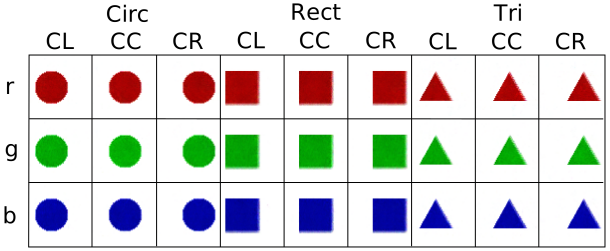
\includegraphics[width=0.75\textwidth]{Figs/shapes/multiword331.png}
\caption{Experiment 1:  Images generated from descriptions with an embedding size of 200.}
\label{fig:331multi}
\end{figure}

Given how well images can be generated from full descriptions, it is unsurpising to see that the MAE has been able to disentangle the descriptions and correctly identify the meanings of each of the words. In \autoref{fig:331shapes} it can be seen that each shape is correctly generated into an image for most embedding sizes. It is difficult to specify which embedding size disentangles the meanings of each word the best as this is purely subjective. I would suggest that and embedding size of 296 neurons grounds the meanings of individual words the best, this is due to it producing the most solid circle, rectangle and triangle across all four runs, in my opinion. 

\begin{figure}[ht]
\centering
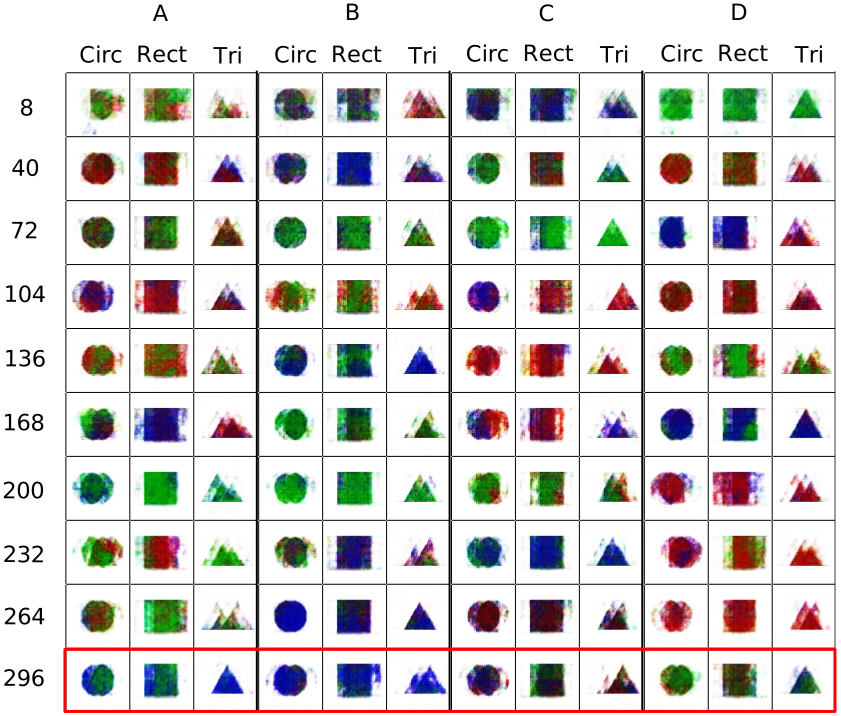
\includegraphics[width=\textwidth]{Figs/shapes/shapes331.png}
\caption{Experiment 1, runs A-D:  Images generated of each shape for different sizes of embedding.}
\label{fig:331shapes}
\end{figure}

The images generated for every word can be found in the suplimental material. As the colour and position are always  correctly learnt across the four runs, they are not shown in the main text.



\paragraph{Multilabel classification}
The MAE gets 100\% accuracy on all descriptions for all testing conditions and all embedding sizes. Accuracy is calculated by counting the number of correctly predicted words and averaging over the entire dataset. For example, given an image of ``big blue circle left'' and the prediction ``small blue circle left'' the accuracy would be 0.75 for that instance as 3 out of 4 words are correctly predicted. A word is considered to be predicted if its neurons activation is above 0.5. As I am using a sigmoid activation function, the output for each neuorn is always between 0 and 1.


\subsubsection{Discussion}
The results of experiment 1 show clearly that the MAE is capable of preforming symbol grounding on this subset of the ArtS dataset. However, it is difficult to make any conclusions about which embedding size gave the best results. Whilst 200 neurons gave the lowest reconstruction error in all testing conditions (see \autoref{tab:res331}), it did not do the best job of disentangling the meanings of each word in the descritptions (see \autoref{fig:331shapes}). 

In the next experiment, we will observe how embedding size affects the reconstruction error and symbol grounding of the MAE when a larger variety of sizes for the objects in the images are available.



\subsection{Experiment 2}
I will now explore how adding more variety to the data affects the quality of reconstruction. To that end, two new sizes of object are added as seen in \autoref{tab:exp2_data}. 

\begin{table}[h]
\centering
\begin{tabular}{|c|c|}
\hline
\textbf{Attribute} & \textbf{Description} \\ \hline \hline
\textbf{Shapes} & \textbf{Corners} \\ \hline
Rectangle & 4\\ \hline
Triangle & 3\\ \hline
Circle & 0\\ \hline 

\textbf{Colours} & \textbf{RGB Values}	\\ \hline	
Red & (75,0,0) - (255, 10, 10)\\ \hline
Green  & (0,75,0) - (10, 255, 10)\\ \hline
Blue   & (0,0,75) - (10, 10, 255)\\ \hline


\textbf{Sizes} & 	\textbf{Length/Radius (pixels)} \\ \hline			  
Big    & 32 - 35  \\ \hline
Medium & 22 - 25 \\ \hline
Small  & 12 - 15 \\ \hline 

\textbf{Positions} & \textbf{Object Centre Coordinate}	\\ \hline					  
Centre Left &(22,32)\\ \hline
Centre Centre & (32,32)\\ \hline
Centre Right &(42,32)\\ \hline				
\end{tabular}
\caption{Experiment 2 data subset.}
\label{tab:exp2_data} 
\end{table}



\subsubsection{Results}
\begin{figure}
\centering
\resizebox{0.9\textwidth}{!}{
\begin{tikzpicture}
    \begin{axis}[
     name=plot1,
     axis x line=middle,
     axis y line=middle,
     enlarge y limits=true,
     enlarge x limits=true,
     legend style={at={(0.5,-0.5)}, anchor=north},
     %xmin=0, xmax=2150,
     %ymin=0, ymax=600,
     %width=15cm, height=8cm,     % size of the image
     grid = major,
     grid style={dashed, gray!30},
     ylabel= Total MSE,
     %ytick={0,0.001,0.002,0.003,0.004,0.005,0.006,0.007,0.008,0.009},
     xlabel= (A) Embedding Size,
     %xtick={6,8,10,12,14,16,18,20,22,24,26,28,30,32,34,35,36,37,38,39,40,41,42,43,44,45,46,47,48,49,50,51,52,53,54,55,56},     
	 xlabel near ticks,
	 ylabel near ticks]
         ] 
    ]
    \addplot table[x = size, y = bimodal, col sep = comma]{csvs/333/total333.csv}; 
    \addplot table[x = size, y = words only, col sep = comma]{csvs/333/total333.csv};
    \addplot table[x = size, y = image only, col sep = comma]{csvs/333/total333.csv};    
    \legend{Bimodal, Words Only, Image Only}
    
    \end{axis}
    
    
     \begin{axis}[
     name=plot2,
     at=(plot1.right of south east), 
     anchor=left of south west,
     axis x line=middle,
     axis y line=middle,
     enlarge y limits=true,
     enlarge x limits=true,
     %legend style={at={(1,0.7)}, anchor=north},
     %xmin=0, xmax=2150,
     %ymin=0, ymax=600,
     %width=15cm, height=8cm,     % size of the image
     grid = major,
     grid style={dashed, gray!30},
     ylabel= Image MSE,
     %ytick={0,0.001,0.002,0.003,0.004,0.005,0.006,0.007,0.008,0.009},
     xlabel= (B) Embedding Size,
     %xtick={6,8,10,12,14,16,18,20,22,24,26,28,30,32,34,35,36,37,38,39,40,41,42,43,44,45,46,47,48,49,50,51,52,53,54,55,56},     
     xlabel near ticks,
	 ylabel near ticks]
         ] 
    ]
    \addplot table[x = size, y = bimodal, col sep = comma]{csvs/333/image333.csv}; 
    \addplot table[x = size, y = words only, col sep = comma]{csvs/333/image333.csv};
    \addplot table[x = size, y = image only, col sep = comma]{csvs/333/image333.csv}; 
       
    %\legend{Bimodal, Words Only, Image Only}
    \end{axis}
    
	
    
    \begin{axis}[
     name=plot3,
     at=(plot2.below south west),
     anchor=above north west,
     axis x line=middle,
     axis y line=middle,
     enlarge y limits=true,
     enlarge x limits=true,
     %legend style={at={(1,0.7)}, anchor=north},
     %xmin=0, xmax=2150,
     %ymin=0, ymax=600,
     %width=15cm, height=8cm,     % size of the image
     grid = major,
     grid style={dashed, gray!30},
     ylabel= Word MSE,
     %ytick={0,0.001,0.002,0.003,0.004,0.005,0.006,0.007,0.008,0.009},
     xlabel= (C) Embedding Size,
     %xtick={6,8,10,12,14,16,18,20,22,24,26,28,30,32,34,35,36,37,38,39,40,41,42,43,44,45,46,47,48,49,50,51,52,53,54,55,56},     
     xlabel near ticks,
	 ylabel near ticks]
         ] 
    ]
    \addplot table[x = size, y = bimodal, col sep = comma]{csvs/333/word333.csv}; 
    \addplot table[x = size, y = words only, col sep = comma]{csvs/333/word333.csv};
    \addplot table[x = size, y = image only, col sep = comma]{csvs/333/word333.csv};    
    %\legend{Bimodal, Words Only, Image Only}
    \end{axis}
    

\end{tikzpicture}
}
\caption{Mean Squared Error for reconstruction of images and words under different testing conditions, Bimodal, Words Only and Image Only for 3 colours, 3 positions and 3 sizes. (A) shows the total MSE, (B) shows the MSE of the image output and (C) shows the MSE of the word output.}
\label{fig:graph333}
\end{figure}

Once again we see that the majority of error comes from the image reconstruction loss by comparing the scales of \autoref{fig:graph333} (B) and (C). The description reconstruction error is larger and less stable with respect to the embedding size than in experiment 1, howver it still remains very small with a scale of $10e^{-4}$.

Interestingly, we see that increasing the embedding size seems to have a positive effect on image reconstruction loss under all testing conditions, though this is still not a very significant increase improvement in the wWrds Only testing condition. \autoref{tab:res333} highlights this, with the best total loss occuring for an embedding size of 296 neurons in all three testing conditions. 
Comparing this to the results of experiment 1, where 200 neurons was the best embedding size with respect to reconstruction loss, it is possible that as the data becomes more complex, the extra neurons allow for representing the multimodal data better.

\begin{table}
\centering
	\begin{tabular}{|c|c|c|c|}
	\hline
	Size & 	Bimodal & 	Image Only 	& 	Words Only \\ \hline
8	&	6.65E-03	$\mypm$	2.00E-04	&	7.37E-03	$\mypm$	3.00E-04	&	6.68E-03	$\mypm$	3.00E-04	\\ \hline
40	&	5.38E-03	$\mypm$	1.00E-04	&	5.66E-03	$\mypm$	1.00E-04	&	5.27E-03	$\mypm$	3.00E-04	\\ \hline
72	&	5.57E-03	$\mypm$	5.00E-04	&	5.90E-03	$\mypm$	5.00E-04	&	6.67E-03	$\mypm$	1.90E-03	\\ \hline
104	&	5.04E-03	$\mypm$	2.00E-04	&	5.52E-03	$\mypm$	2.00E-04	&	4.69E-03	$\mypm$	2.00E-04	\\ \hline
136	&	4.89E-03	$\mypm$	2.00E-04	&	5.53E-03	$\mypm$	1.00E-04	&	4.57E-03	$\mypm$	2.00E-04	\\ \hline
168	&	4.91E-03	$\mypm$	2.00E-04	&	5.51E-03	$\mypm$	1.00E-04	&	4.50E-03	$\mypm$	2.00E-04	\\ \hline
200	&	4.70E-03	$\mypm$	2.00E-04	&	5.47E-03	$\mypm$	1.00E-04	&	4.60E-03	$\mypm$	7.00E-04	\\ \hline
232	&	4.91E-03	$\mypm$	3.00E-04	&	5.66E-03	$\mypm$	2.00E-04	&	4.53E-03	$\mypm$	3.00E-04	\\ \hline
264	&	4.64E-03	$\mypm$	2.00E-04	&	5.46E-03	$\mypm$	1.00E-04	&	4.28E-03	$\mypm$	2.00E-04	\\ \hline
296	&	\textbf{4.41E-03}	$\mypm$	1.00E-04	&	\textbf{5.44E-03}	$\mypm$	1.00E-04	&	\textbf{4.19E-03}	$\mypm$	3.00E-04	\\ \hline



	
	\end{tabular}
\caption{Experiment 2:  Total MSE for a selection of different embedding sizes for the three testing conditions, Bimodal, Image Only and Words Only. An Embedding Size of 296 neurons provides the minimum reconstruction error.}
\label{tab:res333}
\end{table}


\paragraph{Image Generation}

\begin{figure}[h]
\centering
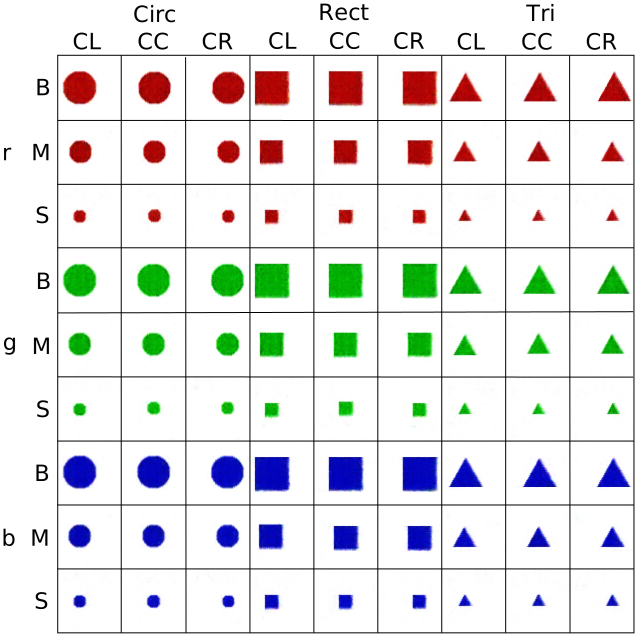
\includegraphics[width=0.75\textwidth]{Figs/shapes/multiword333.png}
\caption{Images generated from descriptions with an embedding size of 296 neurons using the MAE from experiment 2.}
\label{fig:333multi}
\end{figure}

Generating images from full descriptions remains effective as seen in \autoref{fig:333multi}.
With the addition of the extra sizes, generation of images from a single word has become significantly poorer. However, it is still clear that at least some of the words have been succefully grounded. Particularly, the meaning of colours and positions are correctly learnt, with images of distinct colours and positions being generated as seen in \autoref{fig:333single}. 

There is also a clear releationship between the three sizes, shown by the generation of the most coloured pixels for the word ``big'', fewer for ``medium'' and the least for ``small'.

\begin{figure}[h]
\centering
\includegraphics[width=\textwidth]{Figs/shapes/singlelabel333A.png}
\caption{Images generated of each word for different sizes of embedding using the MAE trained in experiment 2 run A.}
\label{fig:333single}
\end{figure} 

The quality of the shapes being generated from the words ``Circle'', ``Rectangle'' and ``Triangle'' has suffered the most. However, there is a clear difference between the three shapes and they do show properties of the shapes they are supposed to be. The ``Circle'' is generally more round than either of the other shapes. The ``Rectangle'' has approxiamtely 4 sides at right angles to one and other, though it is significantly more ``fuzzy'' than in experiment 1. The ``Triangle '' appears triangular, however, for most embedding sizes there appear to be multiple triangles being drawn, this could signify a confusion about where to draw the triangle. I reason that this is the case as in \autoref{fig:2word333} the triangle is significantly more solid when a position is specified. 

Whilst an embedding size of 136 neurons disentangled the meanings of ``Circle'', ``Rectangle'' and ``Triangle'' in run B of experiment 2, this result was not consistent across all four runs (or for any other embedding size) as seen in \autoref{fig:shapes333}. This indicates that the weight initialisation and data selection have an effect on whether the MAE can learn the meanings of the shape names  when additional object sizes are added to the training data.

\begin{figure}
\centering
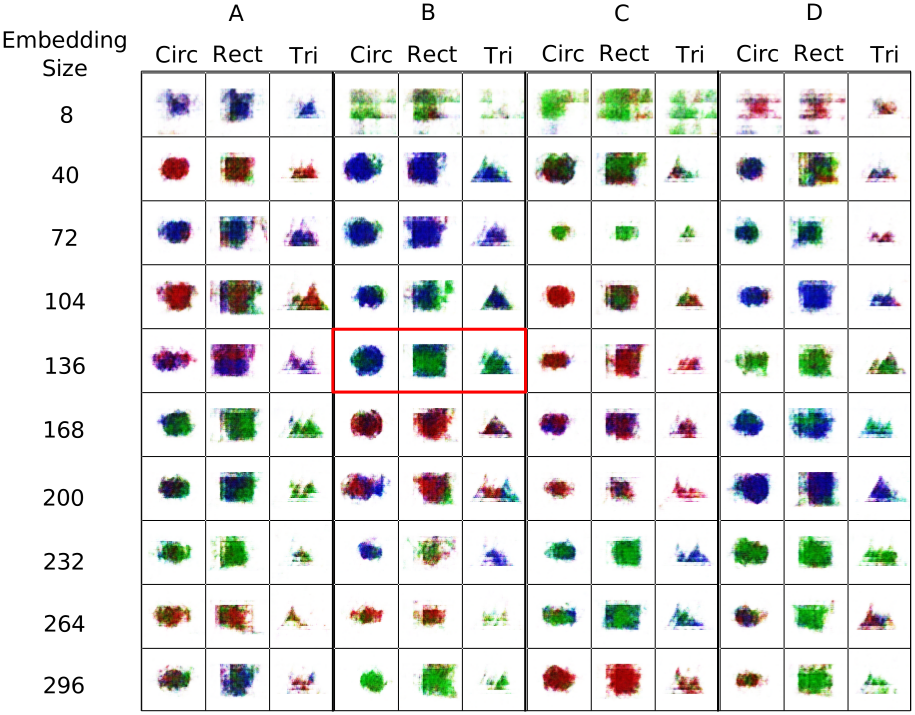
\includegraphics[width=\textwidth]{Figs/shapes/shapes333.png}
\caption{Experiment 2, runs A-D:  Images generated of each shape for different sizes of embedding.}
\label{fig:shapes333}
\end{figure}

Another way to inspect the quality of the learnt embedding is to provide pairs of words to the MAE and observe what it generates as output. \autoref{fig:2word333} shows the output of the MAE trained in run A of experiment 2 (runs B-D can be found in \autoref{appendix:B} with an embedding size of 296 neurons. Here we see clearly that the MAE is correctly generating the words ``Circle'', ``Rectangle'' and ``Triangle'' as well as the other words in its ``vocabulary''. The diagonal of \autoref{fig:2word333} is the equivalent of the bottom row (296) of \autoref{fig:333single}. The addition of a second word allows for the correct generation of the three shapes in different positions and sizes, suggesting that when only the shape is provided as input, the MAE does not know where to draw the shape or how big to draw it. By adding a second word and removing some uncertainty, the output of the MAE is much more defined. This is a particularly strong result in the cas eof when a position is provided in conjuction with either a shape, size or colour. 

\begin{figure}
\centering
\includegraphics[width=\textwidth]{Figs/shapes/2word333A.png}
\caption{Experiment 2, run A:  Images generated using word pairs using an embedding size of 296 neurons.}
\label{fig:2word333}
\end{figure}

\paragraph{Multilabel classification}
Even with the added complexity of the additional sizes, the MAE gets 100\% accuracy as before. 


\subsubsection{Discussion}

Increasing the number of variable attributes in the dataset, i.e. adding the extra sizes, has had a negative affect on the ability of the MAE to disentangle the meanings of each of the words in the descriptions. This is highlighted when the results of experiments 1 and 2 are seen side by side as in \autoref{fig:shapes333v331}.

\begin{figure}
\centering
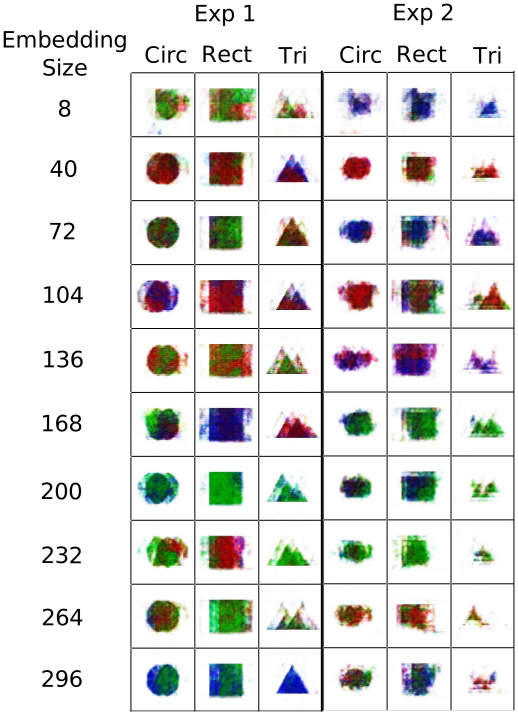
\includegraphics[width=0.5\textwidth]{Figs/shapes/shapes331v333.png}
\caption{Images generated of each shape for different sizes of embedding using the MAEs trained in experiments 1 and 2 run A.}
\label{fig:shapes333v331}
\end{figure} %This issue could likely be solved by the addition of more examples per object.
However, the MAE reamins able to accurately generate images from full descriptions (see \autoref{fig:333multi}). 
An embedding size of 296 neurons gave the all around best performance in experiment 2 and performed the best at symbol grounding in experiment 1, therefore it will be used for the later experiments.

\subsection{Experiment 3}
This experiment adds further vairety to the data, adding an additional 6 positions as seen in \autoref{tab:exp3_data}. In this experiment, we will also observe how incrementally learning these new properties affects the quality of the generated outputs as well as the grounding of the different words from the descriptions. 

Incremental learning is performed by comparing the quality of the output from a MAE trained starting from, random weights, the weights learned in expermiment one and the weights learning in experiment two. This will help answer the fundamental question of whether, having knowledge of the meaning of a subset of words and their image equivalents, aids the learning of new words and their image equivalents.

Unlike in the previous two experiments, the embedding size will be fixed to 296 neurons as this gave the best performance in experiment 2 in terms of loss.


\begin{table}[h]
\centering
\begin{tabular}{|c|c|}
\hline
\textbf{Attribute} & \textbf{Description} \\ \hline \hline
\textbf{Shapes} & \textbf{Corners} \\ \hline
Rectangle & 4\\ \hline
Triangle & 3\\ \hline
Circle & 0\\ \hline 

\textbf{Colours} & \textbf{RGB Values}	\\ \hline	
Red & (75,0,0) - (255, 10, 10)\\ \hline
Green  & (0,75,0) - (10, 255, 10)\\ \hline
Blue   & (0,0,75) - (10, 10, 255)\\ \hline

\textbf{Sizes} & 	\textbf{Length/Radius (pixels)} \\ \hline			  
Big    & 32 - 35  \\ \hline
Medium & 22 - 25 \\ \hline
Small  & 12 - 15 \\ \hline 

\textbf{Positions} & \textbf{Object Centre Coordinate}	\\ \hline					  
Top Left & (22,42)\\ \hline	
Top Centre & (32,42)\\ \hline
Top Right & (42,42)\\ \hline
Centre Left &(22,32)\\ \hline
Centre & (32,32)\\ \hline
Centre Right &(42,32)\\ \hline
Bottom Left & (22,22)\\ \hline
Bottom Centre & (22,42)\\ \hline
Bottom Right & (42,22)\\ \hline				
\end{tabular}
\caption{Experiment 2 data subset.}
\label{tab:exp3_data} 
\end{table}

\subsubsection{Results}
Using the pretrained weights from experiment 1 as a starting point for experiment 3 leads to the lowest reconstruction error as seen in \autoref{tab:res339}. The lower reconstruction error during testing does not translate to improved symbol grounding.

The different starting conditions will be referred to as: Random: randomly initialised weights, Exp1: the weights trained during experiment 1 and Exp2: the weights trained during experiment 2.

\begin{table}[h!]
\centering
	\begin{tabular}{|c|c|c|c|}
	\hline
	Initialisation & 	Bimodal & 	Image Only 	& 	Words Only \\ \hline
	Random	&	5.43E-03	$\mypm$	5.61E-04	&	5.42E-03	$\mypm$	5.60E-04	&	1.00E-06	$\mypm$	7.38E-07	\\ \hline
Exp 1	&	\textbf{5.29E-03}	$\mypm$	4.73E-04	&	\textbf{5.29E-03}	$\mypm$	4.72E-04	&	1.14E-06	$\mypm$	9.20E-07	\\ \hline
Exp 2	&	5.33E-03	$\mypm$	3.12E-04	&	5.33E-03	$\mypm$	3.12E-04	&	\textbf{8.51E-07}	$\mypm$	3.59E-07	\\ \hline

	\end{tabular}
\caption{Experiment 3: Total MSE for different weight initialisations for the three testing conditions, Bimodal, Image Only and Words only.}
\label{tab:res339}
\end{table}


\paragraph{Image Generation}
It is not feasable to show every combination of shape, colour, size and position, so in figure \autoref{fig:339multi} a selection of these combinations are shown.

\begin{figure}[h]
\centering
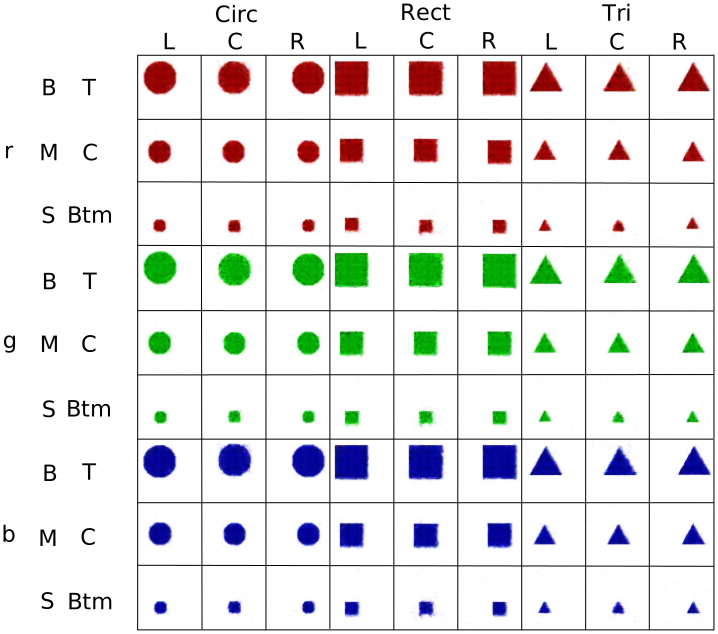
\includegraphics[width=0.75\textwidth]{Figs/shapes/multiword339.png}
\caption{Experiment 3, run A: Images generated from descriptions, starting training from randomly initialised weights.}
\label{fig:339multi}
\end{figure}

The addition of new positions has had an effect on the quality of the images generated from descriptions by the MAE. The images have become blurrier compared to images generated in previous experiments. However they are still easily recognisable as matching their descriptions.

The new positions are correctly learnt with a clear distinction between positions on the top, centre and bottom as well as left, centre and right and their combinations (e.g. bottom right).

\begin{figure}[h]
\centering
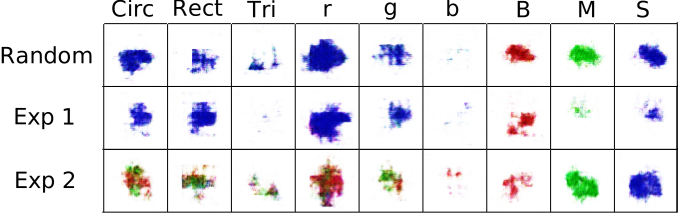
\includegraphics[width=0.75\textwidth]{Figs/shapes/singlelabel339.png}
\caption{Experiment 3, run A: Images generated from shape, colour and size words for different weight initialisation conditions.}
\label{fig:339single}
\end{figure}

\begin{figure}[h]
\centering
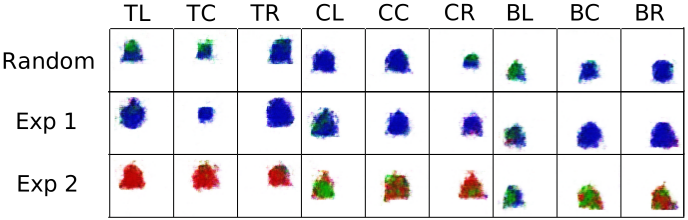
\includegraphics[width=0.75\textwidth]{Figs/shapes/singlelabel339_pos.png}
\caption{Experiment 3, run A: Images generated from each position word for different weight initialisation conditions.}
\label{fig:339single_pos}
\end{figure}


As in experiment 2, the addition of a second word as input, leads to better reconstruction of the images. \autoref{fig:2word339} shows a comparison of the three different weight initialisations after training. It is clear in all three cases that the MAE learns to correctly ground the words ``Circle'', ``Rectangle'' and ``Triangle''. However, in the case of initialising with weights from experiment 1, the transfer learning results in a worse performance than random weights.
\begin{figure}[h]
\centering
\includegraphics[width=\textwidth]{Figs/shapes/2word339_pos.png}
\caption{Experiment 3, run A: Images generated using word pairs.}
\label{fig:2word339}
\end{figure}

Initialising with weights from experiment 2 offers a marginal benifit, with each of the shapes being generally more solid in appearance. Full results from all four runs can be found in the supplimental materials.


\paragraph{Multilabel classification}

\subsubsection{Discussion}
Though the addition of extra positions had a detrimental effect on the generation of images from single words (see \autoref{fig:339single} and \autoref{fig:339single_pos}, the MAE was still able to correctly learn the meaning of all of the words. This becomes particularly apparent when pairs of words are provided as input as in \autoref{fig:2word339}.

The effects of transfer learning, that is taking a developmental approach and transfering weights from a MAE which has already mastered a simpler task are not universal. Whilst the weights from experiment 2 provided a small but noticable benifit when generating images from pairs of words over the random initialisation baseline, the weights from experiment 1 did not. 

\subsection{Experiment 4}
For this experiment we will make use of all of the data in ArtS as shown in \autoref{tab:Arts_desc}. Again I will explore the affects of incremental learning, utilising the prelearned weights of experiments 1 and 2 and 3. This will allow me to examine whether having a larger number of concepts (words and their image equivalents) mastered  helps learning new concepts or whether one can simply learn all concepts simultaneously.

The different starting conditions will be referred to as: Random: randomly initialised weights, Exp1: the weights trained during experiment 1, Exp2: the weights trained during experiment 2, Exp 3: the weights learnt during experiment 3 starting from random initialisation, Exp 1+3: the weights learnt during experiment 3 starting with the weights from experiment 1, Exp 2+3: the weights learnt during experiment 3 starting with the weights from experiment 2.

\subsubsection{Results}

\begin{table}[h!]
\centering
	\begin{tabular}{|c|c|c|c|}
	\hline
	Initialisation & 	Bimodal & 	Image Only 	& 	Words Only \\ \hline
Random	&	3.82E-03	$\mypm$	1.22E-04	&	3.26E-02	$\mypm$	3.65E-02	&	4.00E-03	$\mypm$	9.74E-05	\\ \hline
Exp1	&	3.73E-03	$\mypm$	6.07E-05	&	9.33E-03	$\mypm$	9.71E-03	&	3.91E-03	$\mypm$	3.63E-05	\\ \hline
Exp2	&	3.80E-03	$\mypm$	1.94E-04	&	8.55E-03	$\mypm$	4.70E-03	&	3.96E-03	$\mypm$	2.08E-04	\\ \hline
Exp3	&	3.75E-03	$\mypm$	2.86E-05	&	1.43E-02	$\mypm$	1.22E-02	&	3.93E-03	$\mypm$	4.73E-05	\\ \hline
Exp1+3	&	3.77E-03	$\mypm$	1.40E-04	&	1.62E-02	$\mypm$	1.80E-02	&	3.97E-03	$\mypm$	1.28E-04	\\ \hline
Exp 2+3	&	3.76E-03	$\mypm$	1.23E-04	&	3.31E-02	$\mypm$	5.70E-02	&	3.92E-03	$\mypm$	6.28E-05	\\ \hline



	\end{tabular}
\caption{Experiment 4: Total MSE for different weight initialisations for the three testing conditions, Bimodal, Image Only and Words Only.}
\label{tab:res739}
\end{table}

\paragraph{Image Generation}

\begin{figure}
\centering
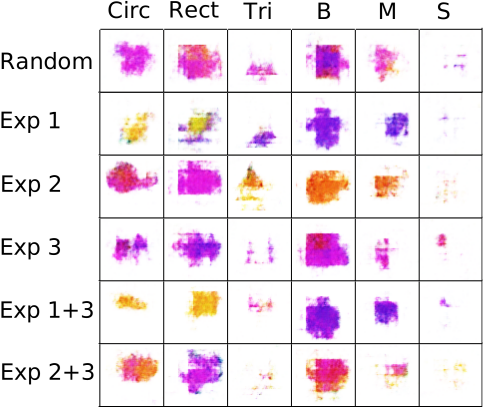
\includegraphics[width=0.75\textwidth]{Figs/shapes/singlelabel739_shape.png}
\caption{Experiment 4, run A: Images generated from shape, colour and size words for different weight initialisation conditions.}
\label{fig:739single_shape}
\end{figure}

\begin{figure}
\centering
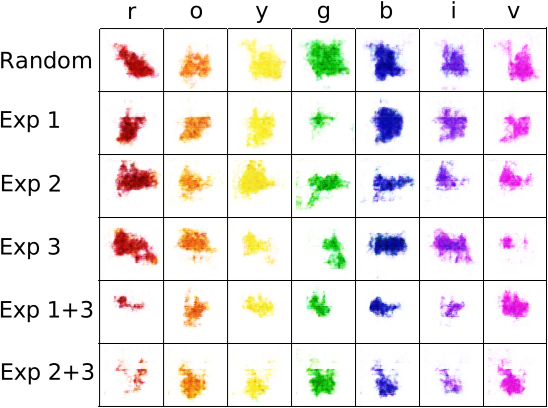
\includegraphics[width=0.75\textwidth]{Figs/shapes/singlelabel739_col.png}
\caption{Experiment 4, run A: Images generated from each colour word for different weight initialisation conditions.}
\label{fig:739single_col}
\end{figure}

\begin{figure}
\centering
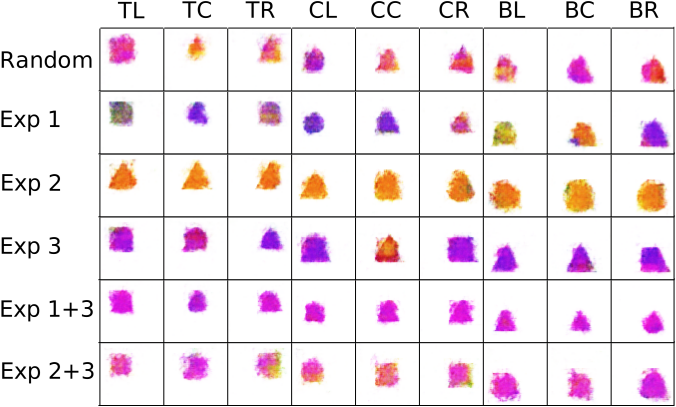
\includegraphics[width=0.75\textwidth]{Figs/shapes/singlelabel739_pos.png}
\caption{Experiment 4, run A: Images generated from each position word for different weight initialisation conditions.}
\label{fig:739single_pos}
\end{figure}



\begin{figure}
\centering
\includegraphics[width=\textwidth]{Figs/shapes/2word739_pos.png}
\caption{Experiment 4, run A: Images generated using word pairs.}
\label{fig:2word739}
\end{figure}



\paragraph{Multilabel classification}


\begin{table}[h!]
\centering
	\begin{tabular}{|c|c|c|c|}
	\hline
	Initialisation & 	Bimodal & 	Image Only 	& 	Words Only \\ \hline
Random	&	1.00E+00	$\mypm$	0.00E+00	&	9.74E-01	$\mypm$	5.91E-02	&	1.00E+00	$\mypm$	0.00E+00\\ \hline
Exp1	&	1.00E+00	$\mypm$	0.00E+00	&	9.95E-01	$\mypm$	2.28E-02	&	1.00E+00	$\mypm$	0.00E+00\\ \hline
Exp2	&	1.00E+00	$\mypm$	2.98E-05	&	9.95E-01	$\mypm$	1.26E-02	&	1.00E+00	$\mypm$	0.00E+00\\ \hline
Exp3	&	1.00E+00	$\mypm$	0.00E+00	&	9.91E-01	$\mypm$	2.49E-02	&	1.00E+00	$\mypm$	0.00E+00\\ \hline
Exp1+3	&	1.00E+00	$\mypm$	0.00E+00	&	9.88E-01	$\mypm$	2.75E-02	&	1.00E+00	$\mypm$	0.00E+00\\ \hline
Exp 2+3	&	1.00E+00	$\mypm$	0.00E+00	&	9.76E-01	$\mypm$	6.72E-02	&	1.00E+00	$\mypm$	0.00E+00\\ \hline


	\end{tabular}
\caption{Experiment 4: Description Accuracy for different weight initialisations for the three testing conditions, Bimodal, Image Only and Words Only}
\label{tab:res739acc}
\end{table}


\subsubsection{Discussion}

\subsection{Experiment 5}
In this experiment I will select certain subsets of objects from the data to omit, such as ``Violet Circles'' or ``Green Triangles''. Then demonstrate how images of these objects can still be generated from their descriptions or through vector arithematic, as well as how images of these objects can be correctly described by the network.

\subsubsection{Results}




\paragraph{Image Generation}
\paragraph{Multilabel classification}
\paragraph{Vector Arithematic}

\subsubsection{Discussion}

\section{Conclusion}

\subsubsection{The effect of  more training examples}
It might seem that the task of learning the relationship between the words of the descriptions and the attributes of the images that they describe, is trivial. Of course, it is for an adult human. Even if the descriptions were given in an unknown language, given very few examples (possibly even less than one example per per shape, colour, size and position combination) an adult could learn the relationship very quickly. Why then, does a neural network need so many examples to get things right?

The root of this issue comes down to two main factors, 1) the underlying probability distribution of the data and 2) the learning method: gradient descent.

To understand what I mean by ``the underlying probability distribution of the data'' let us consider the simple example of rolling a die to decide if it is fair.

How many times should we roll the die before we decide it is fair? If it is a six sided die and it is fair, there should be a $\frac{1}{6}$ chance of rolling each of the numbers 1 to 6. So if we roll it 6 times we should expect to see each number once, however, we most likely won't, that doesn't mean our die is rigged though.

As we roll the die more and more times, we can get a better understanding of the true probability of rolling a given number and therefore get closer to deciding if the die is indeed fair.

\begin{table}
\centering
	\begin{tabular}{|c|c|c|c|c|c|c|c|}
	\hline
	Rolls & 1 & 2 & 3 & 4 & 5 & 6 & $D_{KL}$ \\ \hline
	10 & 0 & 0.2 & 0.2 & 0.3 & 0.2 & 0.1 & 31.36 \\ \hline
	1000 & 0.168 & 0.148 & 0.169 & 0.174 & 0.172 & 0.169 & 10.76 \\ \hline
	100000 & 0.166 & 0.166 & 0.167 & 0.168 & 0.165 & 0.167 & 10.75 \\ \hline
	1000000 & 0.167 & 0.167 & 0.167 & 0.167 & 0.167 & 0.167 & 10.75 \\ \hline
	\end{tabular}
	\caption{Probability distributions generated from rolling a 6 sided die.}
	\label{tab:dieProb}
\end{table}

As we roll the die more and more we will get closer to the actual probability distribution which governs its behaviour. In the limit, the probability for rolling any number should converge to $\frac{1}{6} = 0.167$. Looking at \autoref{tab:dieProb} we can see that the pseudo random number generator (PRNG) I used to simulate rolling a die on my computer, is probably mostly fair. 

Looking at the final column of \autoref{tab:dieProb} we can see that the KL divergence \autoref{eqn:kld}, converges quickly towards 0 for the first 1000 rolls but the slows down and improves only in the 4th or 5th digit after the decimal point. this suggests that the PRNG isn't actually completely fair as even after 10 million rolls, the KL divergence from a uniform distribution is still quite large.

So, how does this relate to the ArtS dataset? Let us replace rolling a die in this example with selecting random images from the ArtS dataset and ask, how much information does this one sample tell me about the underlying distribution of the dataset. If we only select a few images, we are unlikely to capture the entire underlying distribution of the data.
For example, when we select only a few images we might get only dark blue rectangles and no light blue rectangles, so when the neural network sees a light blue rectangle at test time, it won't know that light blue falls into the colour category of ``Blue''. However, as we select more samples, we get a better idea of what the true distribution looks like, just as the estimated probability for rolling a die got closer and closer to uniform the more we rolled it. That means that if we have a larger sample size, we are more likely to see light blue rectnagles as well as dark blue rectangle (and every other shade, shape, size and position combination). 

On to the second point, learning by gradient descent. In \autoref{Chapter3} I explained how gradient descent operates, minimising the cost until it reaches a minimum. However, in practice, it is likely that gradient descent will get stuck in a local minimum, and not find the global minimum. 

\begin{figure}
\begin{center}
\begin{tikzpicture}
\begin{axis}[
axis lines=left,
xtick={90, 180, 270, 360,450,540,630},
xticklabels={},
xlabel={$\Delta w$},
ylabel={$C$},
yticklabels={},
xlabel near ticks,
ylabel near ticks]
\addplot[black, thick, smooth, samples=1000, domain=0:360]{sin(x) + sin(2*\x)+sin(3*\x)+sin(4*\x) + sin(5*\x)};

\addplot[black, thick, smooth, samples=1000, domain=360:630]{-sin(1*(\x-300)) -sin(2*(\x-300)) -sin(3*(\x-300)) -sin(4*(\x-300)) -sin(5*(\x-300))};

\addplot[blue, thick, smooth, samples=1000, domain=0:360]{sin(x) + sin(2*\x)+sin(3*\x)};

\addplot[blue, thick, smooth, samples=1000, domain=360:630]{-sin(1*(\x-270)) -sin(2*(\x-270)) -sin(3*(\x-270))};


\node [red] at (105,375)  (a) {\textbullet};
\node [blue] at (335,5)  (a) {\textbullet};
\node [yellow] at (285,345) (b) {\textbullet};
\legend{Many data, , Few data, }
\end{axis}
    

\end{tikzpicture}
\caption{Visualisation of a cost landscape.}
\label{fig:localminima}
\end{center}
\end{figure}

Consider the red point shown in \autoref{fig:localminima}, if we only have a few examples, gradient descent is suseptable to getting stuck in local minima. However, if we add more training data, the shape of the cost landscape changes. This can remove some local minima whilst also providing more information about the underlying distribution of the data, helping us to find the global minima, the blue point.

\subsubsection{How a developmental approach helps}
When we perform tansfer learning, i.e. pretraining on a different dataset or subset of the data as in experiments 3 and 4, we start at a point in the cost landscape that is hopefully closer to the global minima than starting with randomly secelted wweights.

So, by taking a developmental approach, mastering simple tasks and slowly increasing the difficulty of the tasks we set our neural networks to tackle, we can incrementally approach the global minima. In the case of the ArtS dataset this means incrementally learning to perform bidirectional symbol grounding on a wider variety of words and image properties. Learning new colours, shapes, sizes and positions. 
% Chapter Template

\chapter{Bidirectional Grounding of Real Data} % Main chapter title

\label{Chapter6} % Change X to a consecutive number; for referencing this chapter elsewhere, use \ref{ChapterX}

\lhead{Chapter 6. \emph{Bidirectional Grounding of Real Data}} % Change X to a consecutive number; this is for the header on each page - perhaps a shortened title

%----------------------------------------------------------------------------------------
%	SECTION 1
%----------------------------------------------------------------------------------------
\section{The Difficulties of Real Data}
In the previous chapter I showed that it is possible to use a \ac{MAE} to bidirectionally ground natural language (words) and the visual attributes of images of different objects through \ac{MRL}. However, the data used in the previous chapter is artificial and therefore many of the challenges which real data presents are not present in it. 

When working with real images, there are many factors to consider such as lighting changes, perspective changes and camera noise \cite{keller2016analysis}. These factors were not present in the ArtS dataset, so in this chapter I will show how these impact \ac{MRL} for bidirectional grounding.

\section{Acoustic Packaging}
In order to make use of \ac{MRL} on a robot, it is necessary to have a method to gather and group data from multiple sensory modalities. To do this, I make use of \ac{AP} \cite{schillingmann2009towards, schillingmann2009computational}.

The acoustic packager I implemented for this, is triggered to capture data when sound above a certain threshold is heard by a microphone. Images and audio are recorded with the audio being passed to an \ac{ASR} system to transcribe any speech. The audio, transcription and image together are refered to as an acoustic-package.


\begin{figure}[h]
    \centering
    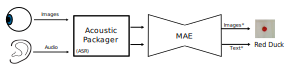
\includegraphics[width=0.7\textwidth]{Figs/chapter6/bimodal_system_schematic.png}
    \caption{System schematic. Data is captured from sensors by an acoustic packager and fed to the multimodal autoencoder.}
    \label{fig:schematic}
\end{figure}

I do not make use of the audio, I use only the transcribed text and images such that the data used in this chapter is analigous to the data used in the previous chapter.

\section{Real Shapes Dataset}

\begin{figure}[h]
    \centering
    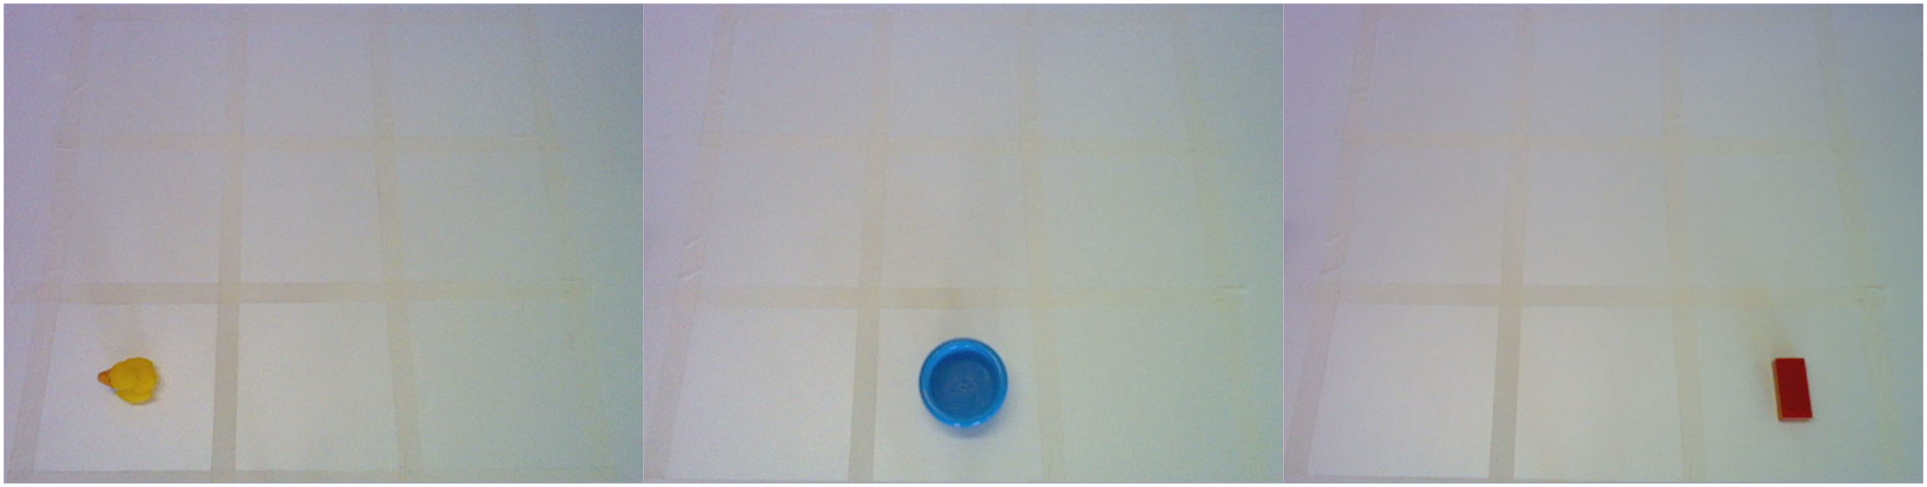
\includegraphics[width=\textwidth]{Figs/chapter6/ReShapeExs.png}
    \caption{Example images from ReShape.}
    \label{fig:ReShape}
\end{figure}

The Real Shapes dataset (ReShape) was created by presenting various objects to a webcam in 9 different positions and giving a short description of the object. \autoref{fig:ReShape} shows example images from ReShape.

\subsection{Dataset Description}
The ReShape dataset contains images and short descriptions of the images.

There are 7 objects, in 10 colours and 3 sizes. Not all objects appear in all 10 colours or all 3 sizes.

\autoref{fig:ReShapeAll} shows cropped, exemplar images for all objects in the ReShape dataset. Not all shape-colour-size combinations are covered in the dataset, hence the large number of blank spaces.

\newpage
\begin{figure}[h!]
    \centering
    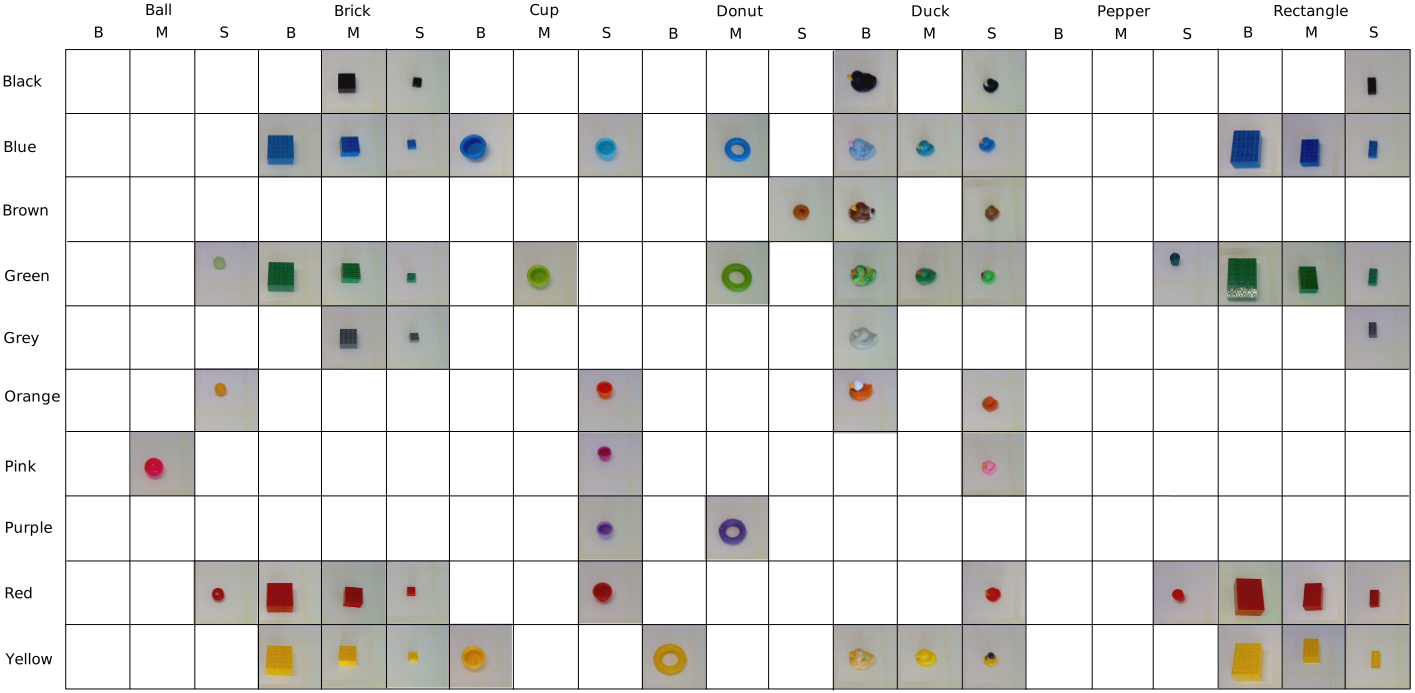
\includegraphics[height=0.7\textwidth, angle=90]{Figs/chapter6/ExemplarAllClasses.png}
    \caption{Exemplar images for all objects in the ReShape dataset.}
    \label{fig:ReShapeAll}
\end{figure}

The dataset was captured in several sessions across multiple days. This is the main source of vairability in the dataset, as different lighting conditions due to whether and time of day has a significant affect on the appearance of images captured by digital cameras \cite{keller2016analysis, keller}\endnote{In \autoref{fig:ReShapeCrop} differences in the lighting conditions are clearly visible with the top left and top centre image having a blue tint.}.



\subsection{Problem Description}
As in the previsous chapter I will be training \acp{MAE} to learn a joint embedding of images and their descriptions. The descriptions only contain a size, shape and colour and not a position as the images are cropped, centring the object in the image, the notion of position is removed from both modalities.

\subsection{Network Description}
I make use of the same network as used in chapter 4 with an embedding size of 296 neurons. 

\section{Experiments with the ReShape dataset}
I will perform two experiments, one with a small subset of the ReShape dataset with complete coverage of every trained and tested combination of colour, object and size is available. The second will make use of a larger variety of objects and colours, however not every combination of object, colour and size is available for training, thus there is not complete coverage, this is similar to experiment 5 in \autoref{Chapter5} where one object-colour combination was excluded from the training data. 

I will also look at the effect of pretraining on the data from experiment 1 and then training for experiment 2. Further to this, two training procedures will be introduced and compared, simple and exemplar.

\subsection{Data Preprocessing}

In the following experiments I do not consider the notion of position and instead crop each image so that the object is roughly centred and consider all objects of the same type to be the equivalent regardless of position (e.g. a \textsc{big blue duck top left} is considered the same as a \textsc{big blue duck center}). As such, the position word is removed from the description of the image and the \ac{MAE} does not contain the position words in its "vocabulary".

\begin{figure}[h]
    \centering
    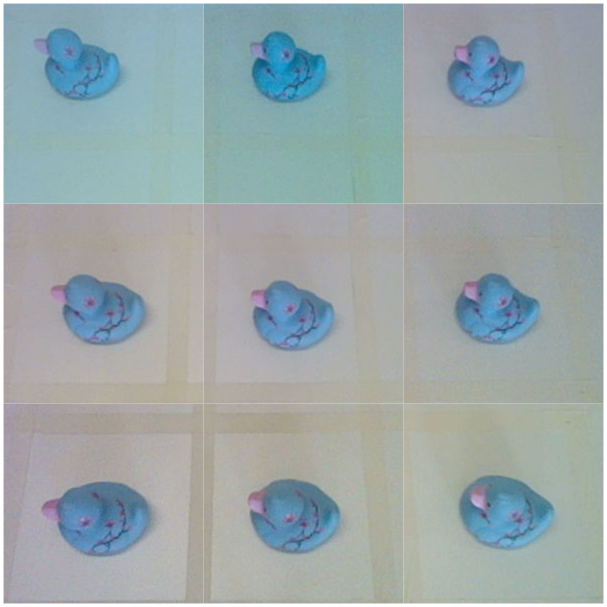
\includegraphics[width=0.7\textwidth]{Figs/chapter6/ReShapeCrop.png}
    \caption{Example cropped images from ReShape.}
    \label{fig:ReShapeCrop}
\end{figure}

Cropping the images is done for three main reasons. 1) this increases the amount of training data for each object by a factor of nine. As the notion of position is removed, the same object in a different position is no longer considered a separate object (unlike in the previous chapter). 2) Cropping reduces the amount of the \ac{MAE}'s field of view which contains the background. This makes it easier for the \ac{MAE} to learn the visual attributes of the objects as less computation is wasted processing the background. 3) Cropping greatly reduces the necessary computation to process a single image as the images are much smaller. Cropping does this without reducing the size of the object in the image unlike resizing the raw image.

Cropping is performed heuristicly, using the position word from the image description to crop out a predefined region. \autoref{fig:CropHeur} shows the regions that each position word relates to for the purposes of cropping.

\begin{figure*}[ht]
    \centering
    \includegraphics[width=0.7\textwidth]{Figs/chapter6/cropHeuristics.png}
    \caption{Regions to crop to given different postion words.}
    \label{fig:CropHeur}
\end{figure*}


%After cropping, their are changes in the visual attributes of the images which are not accounted for in their descriptions. For example, images in top positions, were further from the camera so they appear slightly smaller than those in bottom positions.

\subsection{Training Procedures}

Calculating the average image for each object provides insight into what to expect when generating images in the Words Only test condition.


\begin{figure*}[ht]
    \centering
    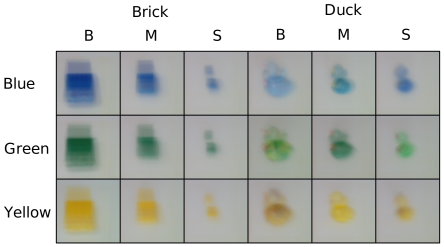
\includegraphics[width=0.7\textwidth]{Figs/chapter6/avgBrickDuckBGY.png}
    \caption{Exp 1: Average of the training images of bricks and ducks in different sizes and colours.}
    \label{fig:AvgBrickDuck}
\end{figure*}

\begin{figure*}[ht]
    \centering
    \includegraphics[width=\textwidth]{Figs/chapter6/avgMost.png}
    \caption{Exp 2: Average of the training images for bricks, cups, donuts, ducks, and rectangles, in different sizes and colours.}
    \label{fig:avgMost}
\end{figure*}

The simple training procedure has the MAE trained to optimise the \ac{MSE} of its output with respect to all of the training data. In the Words Only test condition, the ``best'' images for it to generate are therefore the average images for each object. \autoref{fig:AvgBrickDuck} shows the average image for each object used in experiment 1. \autoref{fig:avgMost} shows the average image for each object in experiment 2.

As the average images are very blurry, it would be useful to have a method which would cause the \ac{MAE} to produce better quality images so that it is easier to inspect which of the visual attributes it has learned to generate correctly.

Using the exemplar training procedure I replace the training image targets with exemplars for each class, when only words are provided as input.

Exemplars are selected by first calculating the average image for each object (\autoref{fig:AvgBrickDuck}, \ref{fig:avgMost}). I then select the training image with the smallest \ac{MSE} from the average image for each object to be the exemplar for that object. 

\autoref{fig:ExmBrickDuck} shows the exemplars used in experiment 1 and \autoref{fig:ExmMost} shows the exemplars for experiment 2.



\subsection{Experiment 1}
Experiment 1 makes use of two shapes in three colours and three sizes. The shapes and colours were selected as they are the only shape-colour combinations that occur in all three sizes in the dataset.

\begin{table}[h]
\centering
\begin{tabular}{|c|c|c|}
\hline

\textbf{Shapes}  & \textbf{Colours} & \textbf{Sizes}\\ \hline \hline
Brick  & Yellow  & Big \\ \hline
Duck   & Green   & Medium \\ \hline
& Blue & Small \\ \hline
			  
			
\end{tabular}
\caption{Experiment 1 data subset.}
\label{tab:6_exp1_data} 
\end{table}

\begin{figure*}[ht]
    \centering
    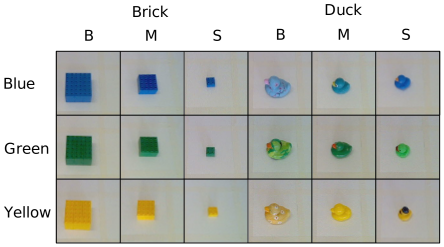
\includegraphics[width=0.7\textwidth]{Figs/chapter6/avgBrickDuckBGYExemplars.png}
    \caption{Exp 1: Exemplar images of bricks and ducks in different sizes and colours.}
    \label{fig:ExmBrickDuck}
\end{figure*}

\subsubsection{Results}

\begin{table}[h!]
\centering
	\begin{tabular}{|c|c|c|c|}
	\hline
\textbf{Training} & 	\textbf{Bimodal} & 	\textbf{Image Only} 	& 	\textbf{Words Only} \\ \hline
Simple & 2.14 $\mypm$ 0.11 & 4.00	$\mypm$ 0.04 & 6.02 $\mypm$ 	0.01 \\ \hline
Exemplar & 2.06 $\mypm$ 0.07 & 3.44 $\mypm$ 0.51 & 7.92	$\mypm$ 0.02 \\ \hline
\end{tabular}
\caption{Exp 1: Total Mean Squared Error for different test conditions and training procedures. (All values are $\times10^{-3}$.)}
\label{tab:6_res_exp1}
\end{table}

Overall, the \ac{MAE} has similar performance in terms of \ac{MSE} using both the simple and exemplar training procedures. Whilst the exemplar method lead to slightly better performance in the Bimodal and Image Only test conditions, this is traded off for worse performance in the Words Only condition. The fact that the \ac{MSE} in the Words only condition is small, shows that the mean image for the training and testing data is very similar.

The similarity between the training and test data is expected in this case as the dataset was created using the same set of objects, in the same location on the same background. As previously mentioned, the main source of variability in the dataset is caused by changes in lighting conditions across the different data-capture sessions. However, this demonstrates an issue with using \ac{MSE} as the cost function to train the \ac{MAE}. If a different example of an object, captured on a different background, from a different angle is used to test the \ac{MAE}, the \ac{MSE} will be very high in the Words Only condition as this image will be very far from the mean image of the training data.

The addition of more training data, with more diverse examples and more detailed descriptions should help. However, as the system is designed for operation on a robot, its absolute performance on a dataset isn't really that important. It is of more worth that the \ac{MAE} generate a "big blue duck" when asked to than to generate the specific "big blue duck" the user had in mind.

\paragraph{Image Generation}

Comparing \autoref{fig:simpleGen_1} and \autoref{fig:AvgBrickDuck} it can be seen that the generated images are almost identical to the average training images for each description when the Simple training procedure is used. 

\begin{figure*}[ht]
    \centering
    \includegraphics[width=0.7\textwidth]{Figs/chapter6/avgBrickDuckBGYGenerated.png}
    \caption{Exp 1: Images generated from full descriptions using the \ac{MAE} trained with the simple procedure.}
    \label{fig:simpleGen_1}
\end{figure*}

Similarly, the Exemplar images from \autoref{fig:ExmBrickDuck} and the images generated by the Exemplar \ac{MAE} in \autoref{fig:exemplarGen_1} are also almost identical.

\begin{figure*}[ht]
    \centering
    \includegraphics[width=0.7\textwidth]{Figs/chapter6/avgBrickDuckBGYGeneratedExemplars.png}
    \caption{Exp 1: Images generated from (only) full descriptions using the MAE trained with the exemplar procedure.}
    \label{fig:exemplarGen_1}
\end{figure*}

These two results show that the \ac{MAE} has overfitted the training data, however this isn't necessarily a bad thing as the generated images are correct for the input descriptions and the \ac{MAE} has perfect accuracy at labelling the test data in the Image Only condition (\autoref{tab:6_res_exp1_acc}).



\begin{figure*}[ht]
    \centering
    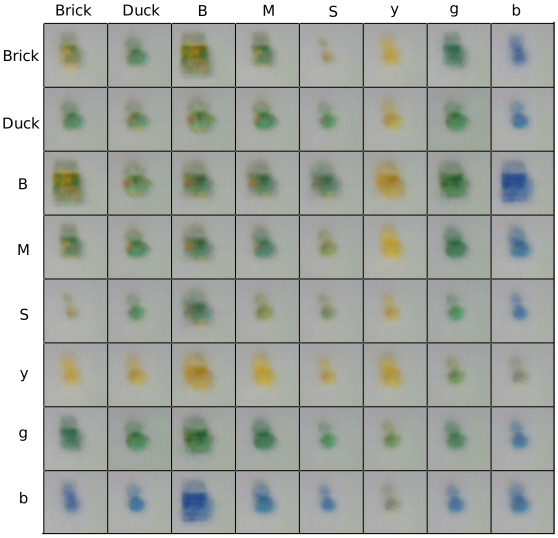
\includegraphics[width=0.7\textwidth]{Figs/chapter6/2wordsSimpleBrickDuck.png}
    \caption{Exp 1: Images generated using word pairs using the MAE trained with the simple procedure.}
    \label{fig:2wordsSimpleBrickDuck}
\end{figure*}

\begin{figure*}[ht]
    \centering
    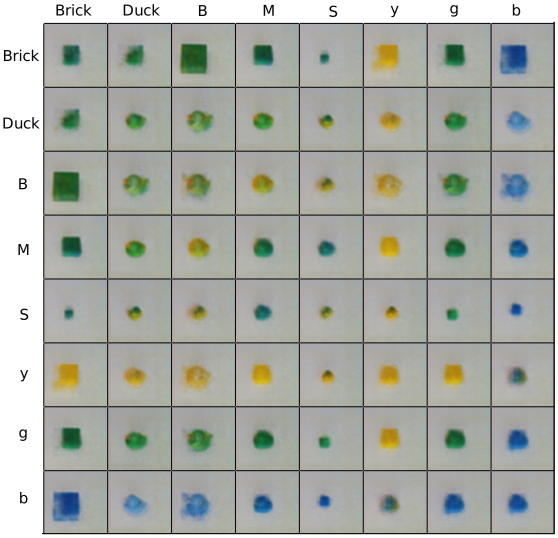
\includegraphics[width=0.7\textwidth]{Figs/chapter6/2wordsExemplarBrickDuck.png}
    \caption{Images generated using word pairs using the MAE trained using image exemplars. (Only words are provided as input.)}
    \label{fig:2wordsExemplarBrickDuck}
\end{figure*}


It is hard to tell how well the \ac{MAE} has learnt the grounded meanings of each individual word when the simple training procedure is used as the generated images are very blurry (\autoref{fig:2wordsSimpleBrickDuck}). The meanings of colours and sizes has been correctly learnt with \textsc{Yellow}, \textsc{Green} and  \textsc{Blue} generating the correct coloured pixels. \textsc{Big} \textsc{Medium} and \textsc{Small} also lead to the correct alteration in number of coloured pixels generated.

In \autoref{fig:2wordsExemplarBrickDuck} as well as the correct grounding of the colours and sizes, we also see that the names of the objects have been correctly grounded, with \textsc{brick} generating a square shape and \textsc{Duck} generating a rubber-duck shape. We also see that detials such as the duck's beak are generated as well as the black top hat on the small yellow duck.

Whilst the generation of the beak is desirable, as all ducks have beaks, the top hat is specific to only two instances of ducks in the training data, a \textsc{big yellow duck} and a \textsc{small yellow duck}. The influence of the top hat can be seen in \autoref{fig:simpleGen_1} with the 
\textsc{big yellow duck} having a black area on its head.

The top hat further highlights that the \ac{MAE} learns to generate the mean image for a given object. So, as with the blurring of the images cuased by the simple training procedure and remedied by the exemplar procedure, is there a method to reduce the introduction of training data specific artifacts like the top hat?

The simplest method to deal with this, would be to increase the complexity of the descriptions of the images. If the duck with a top hat were referred to as "big yellow duck with a top hat", which could be encoded to the network as \textsc{big yellow duck black top hat} by expanding its vocabulary, then distinguishing whether to generate an image of a duck with or without a top hat would be simple.


\paragraph{Multilabel Classification}


\begin{table}[h!]
\centering
	\begin{tabular}{|c|c|c|c|}
	\hline
\textbf{Training }	 & 	\textbf{Bimodal} & \textbf{Image Only} 	& 	\textbf{Words Only} \\ \hline
Simple & 100.00 $\mypm$ 0.00 & 100.00 $\mypm$ 0.00 & 100.00 $\mypm$ 0.00 \\ \hline
Exemplar & 100.00 $\mypm$ 0.00 & 100.00 $\mypm$ 0.00 & 100.00 $\mypm$ 0.00 \\ \hline
	\end{tabular}
\caption{Exp 1: Percentage Description Accuracy for different test conditions and training procedures.}
\label{tab:6_res_exp1_acc}
\end{table}

The \ac{MAE} achieves 100\% accuracy on description generation across all three test conditions. This suggests that the test data has a very similar distribution to the training data. As the test data is images of the same objects captured in the same environment, the only differences between the training data and test data will be small changes in object position and  changes in lighting as the test data was captured on a different day and at a different time of day. Thus, the mean image from the training data for each object is likely very close to the mean image for each object in the test data respectively. It is unlikely that such good performance would be achieved with even small changes to viewing angle or background, which are both constant across the training and test data. However, the addition of more diverse training examples would also alleviate this \cite{keller2016analysis, keller}.

\subsection{Experiment 2}

Experiment 2 makes use of five shapes in five colours and three sizes. The additional shapes and colours were selected as they are represented in most sizes in the dataset.

\begin{table}[h]
\centering
\begin{tabular}{|c|c|c|}
\hline

\textbf{Shapes}  & \textbf{Colours} & \textbf{Sizes}\\ \hline \hline
Brick  & Yellow  & Big \\ \hline
Duck   & Green   & Medium \\ \hline
Donut & Blue & Small \\ \hline
Cup  & Red & \\ \hline
Rectangle & Black & \\ \hline

\end{tabular}
\caption{Experiment 2 data subset.}
\label{tab:6_exp2_data} 
\end{table}

\begin{figure*}[ht]
    \centering
    \includegraphics[width=\textwidth]{Figs/chapter6/exemplarMost.png}
    \caption{Exp 2: Exemplar images of bricks, cups, donuts, ducks, and rectangles, in different sizes and colours.}
    \label{fig:ExmMost}
\end{figure*}


\subsubsection{Results}

\begin{table}[h!]
\centering
	\begin{tabular}{|c|c|c|c|}
	\hline
\textbf{Training} & 	\textbf{Bimodal} & 	\textbf{Image Only} 	& 	\textbf{Words Only} \\ \hline
Simple &  2.14 $\mypm$	0.07 & 3.89 $\mypm$	0.62 & 6.08 $\mypm$ 0.01 \\ \hline
Exemplar & 2.30 $\mypm$ 0.07 & 3.67 $\mypm$ 0.23
& 10.51	$\mypm$ 0.01 \\ \hline

\end{tabular}
\caption{Exp 2: Total Mean Squared Error for different test conditions and training procedures. (All values are $\times10^{-3}$.)}
\label{tab:6_res_exp2}
\end{table}


\subsubsection{Image Generation}
The \ac{MAE} is able to generalise to unseen combinations of attributes, confirming the result found in the final experiment of the previous chapter (Experiment 5 \autoref{Chapter5}). However, in this case, we have many more missing examples. \autoref{fig:mostExemplarGen} shows the images generated from full descriptions by the \ac{MAE} trained using exemplars. The red borders show images which have exemplars; those without red borders are not seen in the training data, yet the \ac{MAE} is still able to produce good approximations of these objects.

The clearest example of generalisation to unseen objects is the generation of donuts in \autoref{fig:mostExemplarGen}. Despite only having 3 examples of donuts, the \ac{MAE} is able to generate images of donuts in different colours and sizes.  

The quality of the generated images for unseen objects is strongly linked to whether there is a similar example to the requested image. For example, the \textsc{big green donut} and \textsc{small green donut} are of a higher quality than the \textsc{big red donut} and \textsc{small red donut}. This is due to the existence of a \textsc{medium green donut} in the training data. As there are no red donuts in the training data, the \ac{MAE} must rely on its knowledge of the meanings of the individual words \textsc{big}, \textsc{red} and \textsc{donut} to generate an image of a \textsc{big red donut}. For the \textsc{big green donut}, the \ac{MAE} has an example of a \textsc{medium green donut} so it must only alter the size of the object in the image, it does not need to generate the image from the individual words \textsc{big}, \textsc{green} and \textsc{donut}.

In general the \ac{MAE} shows its worst performance on \textsc{black} objects, this is likely due to the reletively few examples of black objects in the training data (5 for black versus 8 for red, 11 for green and yellow and 12 for blue).

\begin{figure*}[ht]
    \centering
    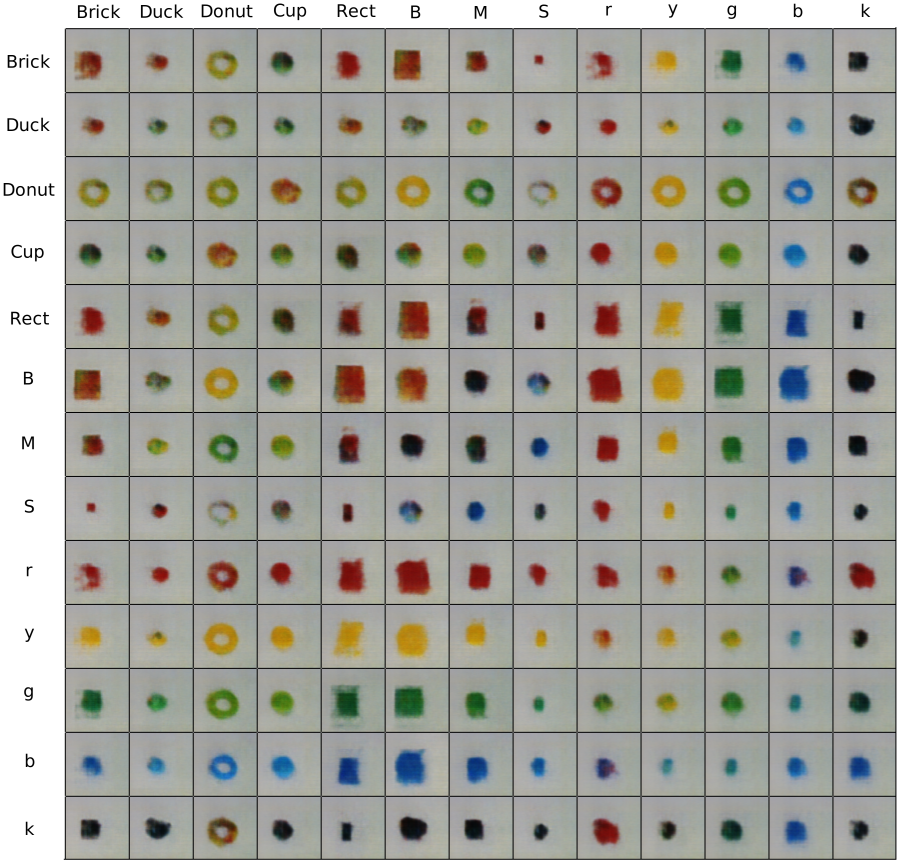
\includegraphics[width=\textwidth]{Figs/chapter6/2wordsMostExemplar.png}
    \caption{Exp 2: Images generated using word pairs using the \ac{MAE} trained using image exemplars when only words are provided as input.}
    \label{fig:2wordsMostExemplar}
\end{figure*}


In \autoref{fig:2wordsMostExemplar} we can see the output of the \ac{MAE}'s image output when only two words are given as input. The meaning of the different colours has been learnt with all images in the red (r), yellow, (y) green (g) blue (b) and black (k) rows and columns having their appropriate colour except when two colours are given as input (e.g. "yellow green") which does not have a true meaning in this instance. We do however see that some colours are more dominant than others, (in order, y, g, b, r, k), this is likely due to their prominence in the dataset, with more examples of yellow, green and blue objects than either red or black objects. 

Yellow dominating over blue and green is likely due to less variance in the shade of yellow in the dataset vs the variance in shades of blue and green (similarly for green dominating over blue). This can be seen clearly in \autoref{fig:ExmMost} where nearly all of the yellow objects have the same shade of yellow compared to blue where there is a spectrum of blues from dark to light blue.

The sizes have been correctly learnt with big (B) images having more coloured pixels than medium (M) images which in turn have more coloured pixels than small (S) images.

The different shapes have been learnt to different degrees. For example, the Donut is clearly a ring in all valid cases (i.e. when only one object name is provided as input).



\paragraph{Multilabel Classification}

\begin{figure*}[ht]
    \centering
    \includegraphics[width=\textwidth]{Figs/chapter6/exemplarMostGenerated.png}
    \caption{Exp 2: Images generated from full descriptions using the \ac{MAE} trained with the exemplar procedure. Red borders show objects with exemplar images.}
    \label{fig:mostExemplarGen}
\end{figure*}

In \autoref{tab:6_res_exp2} we can see the total \ac{MSE} for generation of images and text in the three different test conditions. In all three condition the \ac{MSE} is very low and has low variance across the four cross validation trials.

\paragraph{Description Accuracy}
\begin{table}[h!]
\centering
	\begin{tabular}{|c|c|c|c|}
	\hline
\textbf{Training}	 & 	\textbf{Bimodal} & \textbf{Image Only} 	& 	\textbf{Words Only} \\ \hline
Simple &  100.00 $\mypm$ 0.00 & 100.00 $\mypm$ 0.00 & 100.00 $\mypm$ 0.00 \\ \hline
Exemplar & 100.00 $\mypm$ 0.00 & 100.00 $\mypm$ 0.00 & 100.00 $\mypm$ 0.00 \\ \hline
\end{tabular}
\caption{Accuracy}
\label{tab:6_res_exp2_acc}
\end{table}


In all three test conditions the \ac{MAE} correctly generates descriptions with 100\% accuracy (\autoref{tab:6_res_exp2_acc}. This is due to the similarity of the training and test data, as previously discussed.

\subsection{Discussion}

Applying \ac{MRL} to real data presents many new challenges as compared to when it is applied to the ArtS dataset. Whilst real images have much more noise in them than artificially generated images, the more important difference between Arts and ReShape is that there are many visual attributes in the ReShape dataset which are not accounted for in the image descriptions.

This showed up as the introduction of image artifacts such as the top hat on the yellow duck in both experiments 1 and 2 as well as the blurring of images generated when class exemplars were not used in training. In the ArtS dataset each object was fully described by its description, whereas in ReShape, there are changes in perspective due to the different locations which images were captured at and visual textures such as patterns on the ducks beyond their primary colour (for example, the duck in \autoref{fig:CropHeur} has a floral pattern but is only described as a \textsc{Big Blue Duck}).

There is also the issue of not having full coverage of every size, colour and shape combination. Whilst \ac{MRL} has been demonstrated to cope well with missing examples, correctly generating images of unseen objects, these images are lower quality than the images generated for objects which have exemplars. The fewer examples of a particular shape, colour or size, the worse the image generation for that attribute. \autoref{fig:mostExemplarGen} highlights this, where \textsc{big black donut} is generated as a \textsc{big brown/yellow donut} as the MAE does not have a strong representation of the colour black and only has three examples of donuts.



\section{Summary}
This chapter focused on how \ac{MRL} could be applied to real data, demonstrating how it can be used to solve the symbol grounding problem in an unsupervised manner.
To that end, I have demonstrated that \ac{MRL} can be used to perform bidirectional grounding of images and text. Further to this I shown that \ac{MRL} can generalise to unseen examples, correctly generating images of unseen objects.

The ability of the \ac{MAE} to generate images of unseen objects like the \textsc{Big Red Donut} is very exciting. This result hints at the possibility to develop grounded models capable of understanding more diverse visual attributes and larger numbers of objects.

These experiments present a starting point from which more powerful models can be built through the use of larger datasets as well as through the incorporation of advanced  \ac{ANN} techniques such as dilated and multiscale convolutions, and residual connections. The addition of these types of features to the \ac{MAE} architecture could allow for stronger models of image feature scale and shape and how these relate to the words which describe them.

Further discussion of the results from this chapter has been published in \cite{sheppard2020multimodal}.
\theendnotes 
% Chapter Template

\chapter{Conclusion} % Main chapter title

\label{Chapter7} % Change X to a consecutive number; for referencing this chapter elsewhere, use \ref{ChapterX}

\lhead{Chapter 7. \emph{Conclusion}} % Change X to a consecutive number; this is for the header on each page - perhaps a shortened title

%----------------------------------------------------------------------------------------
%	SECTION 1
%----------------------------------------------------------------------------------------

\section{Summary of Important Points}
Through the course of the experiments shown in \autoref{Chapter4}, \autoref{Chapter5} and \autoref{Chapter6}, I have demonstrated that  \ac{MRL} can be used to learn a grounded representation of different data modalities in an unsupervised manner.

This representation has been demonstrated to fit the criteria layed out by Bengio et al. in \cite{repRev}. Particularly, the representation has been demonstrated to have Manifolds which can be manipulated through vector arithmetic to make predictable and meaningful changes in the output.

In some datasets, such as MNIST and ArtS, it is possible to generate image prototypes for each class/word in the \ac{MAE}'s vocabulary. For MNIST, this came in the form of prototypical versions of each digit and for ArtS, images of each colour, shape and size can be generated individually.

This is also possible for the ReShape dataset However, due to the larger variability of training examples, the prototypes are very blurry. By using a class exemplar for each object, the \ac{MAE} was able to learn to generate non-blurry prototypes for each of the visual attributes.

I also demonstrated that \ac{MRL} can be used to generate accurate object descriptions of both real and artificial images. As well as that using \ac{MRL} can led to improvements in classification accuracy as seen in \autoref{Chapter4}.


\section{Conclusion}
\ac{MRL} has been shown to be a powerful technique and presents an area worthy of futher study. Whilst the findings of the experiments in this thesis are exciting, further work is needed to apply \ac{MRL} in a real world setting.


% Chapter Template

\chapter{Future Work} % Main chapter title

\label{Chapter8} % Change X to a consecutive number; for referencing this chapter elsewhere, use \ref{ChapterX}

\lhead{Chapter 8. \emph{Future Work}} % Change X to a consecutive number; this is for the header on each page - perhaps a shortened title

%----------------------------------------------------------------------------------------
%	SECTION 1
%----------------------------------------------------------------------------------------

\section{What Comes Next?}
The experiments layed out in the previous chapters have shown that \ac{MRL} using \acp{MAE} allows for the unsupervised learning of a grounded representation of images and language. How then, can this be used to improve robotic technologies?

I see many potential applications for \ac{MRL} within the field of \ac{HRI}. \autoref{fig:fsm} shows an example of how the \ac{MAE} can be included in a robotic system.


\begin{figure}
\centering
\includegraphics[width=\textwidth]{Figs/futureWork/fsm.png}
\caption{An example of how the \ac{MAE} can be used as part of a robotic system.}
\label{fig:fsm}
\end{figure}

Consider the scenario of a human interacting with a robot to teach it a set of objects and their visual attributes as well as the words used to describe the objects and their visual attributes. In a laboratory setting it is feasable to have only a single object in view at any given time. This is not true for real world scenarios. However, with the introduction of a \ac{FSM} controlled via a \ac{NLU} module, it is simple to use a \ac{MAE} trained with \ac{MRL} to discern which object is being referred to by the human. This is demonstrated in \autoref{fig:disamb}

\begin{figure}
\centering
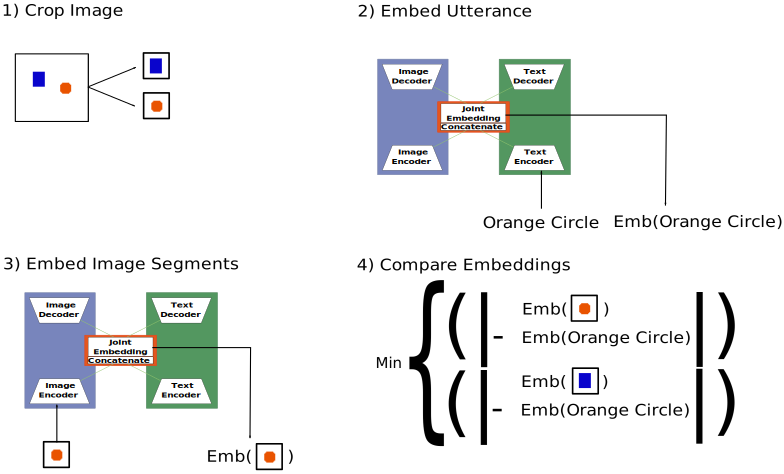
\includegraphics[width=\textwidth]{Figs/shapes/findingRefferant.png}
\caption{An example of using an MAE trained with MRL to disambiguate which object is being referred to in a scene.}
\label{fig:disamb}
\end{figure}

First, the image is split into patches, this can be done naively by sliding a window over the image and processing each patch. However this is not very computationally efficient and is likely to give ambiguous results, depending on the stride of the window, as multiple image patches may contain parts of the object of interest. Therefore it would be sensible to make use of an object detector such as Yolo v3 \cite{redmon2018yolov3} to predict object bounding boxes.

Comparing the embedding of each image patch to the embedding of the query, the image patch of interest should have the smallest \ac{MSE} between it and the query.

In order for the scenario depicted in \ref{fig:disamb}, an \ac{NLU} module must be trained to extract the Intent of the human's utterance as well as any Entities which the human refers to. Fortunately, these types of \acp{NLU} are easily built using open source libraries like Rasa \cite{rasa}.



Developing the infrastructure for this type of scenario would allow for the exploration of questions such as:

\begin{itemize}
\item How many training examples does the \ac{MAE} require to operate accurately?
\item Is their an upper limit on the number of objects, visual attributes and words which the \ac{MAE} can learn?
\item How does regenerating a missing modality affect classification accuracy? Can the embedding of the regnerated missing modality be exploited to enhance  multimodal recognition techniques?
\end{itemize}

I believe \ac{MRL} can be used as a general tool for facilitating \ac{HRI} experiments, with the \ac{MAE} providing a piece of a cognitive architecture which translates low level sensory percepts (vision) to high level symbols (language).


%-----------------------------------
%	SUBSECTION 1
%-----------------------------------
 


\appendix 
\lhead{Appendix B \emph{Sensory Redundancy}}
\label{Appendix:A}
\begin{landscape}
\begin{table}[p]
\centering
		\begin{tabular}{|c|c|c|c|c|c|c|c|}
		\hline
		Model & Training & Testing & Im MSE & MFCC MSE & Lb MSE & Total MSE & Acc \\
		\hline
		Image AE & Im & Im & 0.0027	&	&0.0019	& 0.0046	&	0.9883\\ \hline
		MFCC AE & MFCC & MFCC & 	&0.0113	&	0.0026	&	0.0139	& 0.9832\\ \hline
		\multirow{6}{*}{Add MAE} & \multirow{3}{*}{Bi} & Bi &	0.0030	&	0.0401	&	0.0006	&	0.0437	&0.9967\\ \cline{3-8}
		&& Im &	0.0076	&	0.1641	&	0.0763	&	0.2479	&0.4501 \\ \cline{3-8}
		&& MFCC &	0.1138	&	0.0399	&	0.0057	&	0.1594	&0.9624 \\ \cline{2-8}
		& \multirow{3}{*}{RD} & Bi&	0.0033	&	0.0176	&	0.0001	&	0.0210	& 0.9993 \\ \cline{3-8}
		&& Im &	0.0027	&	0.0455	&	0.0025	&	0.0508	& 0.9834\\ \cline{3-8}
		&& MFCC & 0.0556	&	0.0166	&	0.0031	&	0.0752	&	0.9789 \\ \hline
		
		\multirow{6}{*}{Concat MAE} & \multirow{3}{*}{Bi} & Bi &	0.0031	&	0.0423	&	0.0009	& 0.0462	&	0.9945 \\ \cline{3-8}
		&& Im &	0.0055	&	0.2029	&	0.0843	&	0.2927	&	0.3496 \\ \cline{3-8}
		&& MFCC &0.1138	&	0.0420	&	0.0079	&0.1637	&	0.9455 \\ \cline{2-8}
		& \multirow{3}{*}{RD} & Bi &	0.0030	&	0.0426	&	0.0002	&	0.0458	&0.9986 \\ \cline{3-8}
		&& Im &	0.0026	&	0.0737	&	0.0026	& 0.0788	&	0.9834
\\ \cline{3-8}
		&& MFCC &	0.0554	&	0.0416	&	0.0026	&	0.0996	&0.9827
 \\ \hline
		\end{tabular}
		\caption{Results from the combined MNIST Handwritten Digits and UCU Arabic Spoken Digits}
		\label{tab:mnist_ucu_master_res}
\end{table}		
\end{landscape}	


\lhead{Appendix B \emph{Magical Vectors and where to find them}}
\label{appendix:B}
This appendix contains extra figures from \autoref{Chapter5}
\begin{figure}
\centering
\includegraphics[width=0.75\textwidth]{Figs/shapes/singlelabel331A.png}
\caption{Images generated of each word for different sizes of embedding using the MAE trained in experiment 1 run A.}
\label{fig:331singleA}
\end{figure}
\begin{figure}
\centering
\includegraphics[width=0.75\textwidth]{Figs/shapes/singlelabel331B.png}
\caption{Images generated of each word for different sizes of embedding using the MAE trained in experiment 1 run B.}
\label{fig:331singleB}
\end{figure}
\begin{figure}
\centering
\includegraphics[width=0.75\textwidth]{Figs/shapes/singlelabel331C.png}
\caption{Images generated of each word for different sizes of embedding using the MAE trained in experiment 1 run C.}
\label{fig:331singleC}
\end{figure}
\begin{figure}
\centering
\includegraphics[width=0.75\textwidth]{Figs/shapes/singlelabel331D.png}
\caption{Images generated of each word for different sizes of embedding using the MAE trained in experiment 1 run D.}
\label{fig:331singleD}
\end{figure}


\begin{figure}
\centering
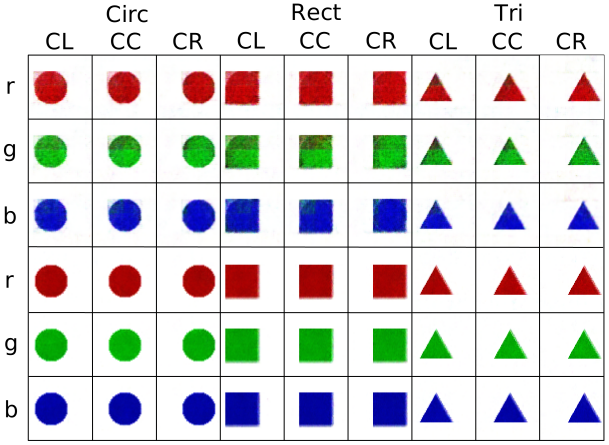
\includegraphics[width=0.75\textwidth]{Figs/shapes/331_8v200.png}
\caption{Images generated from descriptions with an embedding size of 8 or 200.}
\label{fig:8vs200}
\end{figure}


\begin{figure}
\centering
\includegraphics[width=0.75\textwidth]{Figs/shapes/singlelabel333A.png}
\caption{Images generated of each word for different sizes of embedding using the MAE trained in experiment 2 run A.}
\label{fig:333singleA}
\end{figure}
\begin{figure}
\centering
\includegraphics[width=0.75\textwidth]{Figs/shapes/singlelabel333B.png}
\caption{Images generated of each word for different sizes of embedding using the MAE trained in experiment 2 run B.}
\label{fig:333singleB}
\end{figure}
\begin{figure}
\centering
\includegraphics[width=0.75\textwidth]{Figs/shapes/singlelabel333C.png}
\caption{Images generated of each word for different sizes of embedding using the MAE trained in experiment 2 run C.}
\label{fig:333singleC}
\end{figure}
\begin{figure}
\centering
\includegraphics[width=0.75\textwidth]{Figs/shapes/singlelabel333D.png}
\caption{Images generated of each word for different sizes of embedding using the MAE trained in experiment 2 run D.}
\label{fig:333singleD}
\end{figure}

\begin{figure}
\centering
\includegraphics[width=0.75\textwidth]{Figs/shapes/2word333A.png}
\caption{Images generated using word pairs using an embedding size of 296 neurons from experiment 2 run A.}
\label{fig:2word333A}
\end{figure}

\begin{figure}
\centering
\includegraphics[width=0.75\textwidth]{Figs/shapes/2word333B.png}
\caption{Images generated using word pairs using an embedding size of 296 neurons from experiment 2 run B.}
\label{fig:2word333B}
\end{figure}

\begin{figure}
\centering
\includegraphics[width=0.75\textwidth]{Figs/shapes/2word333C.png}
\caption{Images generated using word pairs using an embedding size of 296 neurons from experiment 2 run C.}
\label{fig:2word333C}
\end{figure}

\begin{figure}
\centering
\includegraphics[width=0.75\textwidth]{Figs/shapes/2word333D.png}
\caption{Images generated using word pairs using an embedding size of 296 neurons from experiment 2 run D.}
\label{fig:2word333D}
\end{figure}



\begin{figure}
\centering
\includegraphics[width=\textwidth]{Figs/shapes/2word339A.png}
\caption{Images generated using word pairs using a MAE initialised with random weights for experiment 3 run A.}
\label{fig:2word339A}
\end{figure}

\begin{figure}
\centering
\includegraphics[width=\textwidth]{Figs/shapes/2word339B.png}
\caption{Images generated using word pairs using a MAE initialised with random weights for experiment 3 run B.}
\label{fig:2word339B}
\end{figure}

\begin{figure}
\centering
\includegraphics[width=\textwidth]{Figs/shapes/2word339C.png}
\caption{Images generated using word pairs using a MAE initialised with random weights for experiment 3 run C.}
\label{fig:2word339C}
\end{figure}

\begin{figure}
\centering
\includegraphics[width=\textwidth]{Figs/shapes/2word339D.png}
\caption{Images generated using word pairs using a MAE initialised with random weights for experiment 3 run D.}
\label{fig:2word339D}
\end{figure}

\begin{figure}
\centering
\includegraphics[width=\textwidth]{Figs/shapes/2word339A1.png}
\caption{Images generated using word pairs using a MAE initialised with weights from experiment 1 for experiment 3 run A.}
\label{fig:2word339A1}
\end{figure}

\begin{figure}
\centering
\includegraphics[width=\textwidth]{Figs/shapes/2word339B1.png}
\caption{Images generated using word pairs using a MAE initialised with weights from experiment 1 forexperiment 3 run B.}
\label{fig:2word339B1}
\end{figure}

\begin{figure}
\centering
\includegraphics[width=\textwidth]{Figs/shapes/2word339C1.png}
\caption{Images generated using word pairs using a MAE initialised with weights from experiment 1 for experiment 3 run C.}
\label{fig:2word339C1}
\end{figure}

\begin{figure}
\centering
\includegraphics[width=\textwidth]{Figs/shapes/2word339D1.png}
\caption{Images generated using word pairs using a MAE initialised with weights from experiment 1 for experiment 3 run D.}
\label{fig:2word339D1}
\end{figure}

\begin{figure}
\centering
\includegraphics[width=\textwidth]{Figs/shapes/2word339A2.png}
\caption{Images generated using word pairs using a MAE initialised with weights from experiment 2 for experiment 3 run A.}
\label{fig:2word339A2}
\end{figure}

\begin{figure}
\centering
\includegraphics[width=\textwidth]{Figs/shapes/2word339B2.png}
\caption{Images generated using word pairs using a MAE initialised with weights from experiment 2 forexperiment 3 run B.}
\label{fig:2word339B2}
\end{figure}

\begin{figure}
\centering
\includegraphics[width=\textwidth]{Figs/shapes/2word339C2.png}
\caption{Images generated using word pairs using a MAE initialised with weights from experiment 2 for experiment 3 run C.}
\label{fig:2word339C2}
\end{figure}

\begin{figure}
\centering
\includegraphics[width=\textwidth]{Figs/shapes/2word339D2.png}
\caption{Images generated using word pairs using a MAE initialised with weights from experiment 2 for experiment 3 run D.}
\label{fig:2word339D2}
\end{figure}




\begin{figure}
\centering
\includegraphics[width=\textwidth]{Figs/shapes/2word739A.png}
\caption{Images generated using word pairs using a MAE initialised with random weights for experiment 4 run A.}
\label{fig:2word739A}
\end{figure}

\begin{figure}
\centering
\includegraphics[width=\textwidth]{Figs/shapes/2word739B.png}
\caption{Images generated using word pairs using a MAE initialised with random weights for experiment 4 run B.}
\label{fig:2word739B}
\end{figure}

\begin{figure}
\centering
\includegraphics[width=\textwidth]{Figs/shapes/2word739C.png}
\caption{Images generated using word pairs using a MAE initialised with random weights for experiment 4 run C.}
\label{fig:2word739C}
\end{figure}

\begin{figure}
\centering
\includegraphics[width=\textwidth]{Figs/shapes/2word739D.png}
\caption{Images generated using word pairs using a MAE initialised with random weights for experiment 4 run D.}
\label{fig:2word739D}
\end{figure}


\begin{figure}
\centering
\includegraphics[width=\textwidth]{Figs/shapes/2word739A1.png}
\caption{Images generated using word pairs using a MAE initialised with weights from experiment 1 for experiment 4 run A.}
\label{fig:2word739A1}
\end{figure}

\begin{figure}
\centering
\includegraphics[width=\textwidth]{Figs/shapes/2word739B1.png}
\caption{Images generated using word pairs using a MAE initialised with weights from experiment 1 for experiment 4 run B.}
\label{fig:2word739B1}
\end{figure}

\begin{figure}
\centering
\includegraphics[width=\textwidth]{Figs/shapes/2word739C1.png}
\caption{Images generated using word pairs using a MAE initialised with weights from experiment 1 for experiment 4 run C.}
\label{fig:2word739C1}
\end{figure}

\begin{figure}
\centering
\includegraphics[width=\textwidth]{Figs/shapes/2word739D1.png}
\caption{Images generated using word pairs using a MAE initialised with weights from experiment 1 for experiment 4 run D.}
\label{fig:2word739D1}
\end{figure}

\begin{figure}
\centering
\includegraphics[width=\textwidth]{Figs/shapes/2word739A2.png}
\caption{Images generated using word pairs using a MAE initialised with weights from experiment 2 for experiment 4 run A.}
\label{fig:2word739A2}
\end{figure}

\begin{figure}
\centering
\includegraphics[width=\textwidth]{Figs/shapes/2word739B2.png}
\caption{Images generated using word pairs using a MAE initialised with weights from experiment 2 for experiment 4 run B.}
\label{fig:2word739B2}
\end{figure}

\begin{figure}
\centering
\includegraphics[width=\textwidth]{Figs/shapes/2word739C2.png}
\caption{Images generated using word pairs using a MAE initialised with weights from experiment 2 for experiment 4 run C.}
\label{fig:2word739C2}
\end{figure}

\begin{figure}
\centering
\includegraphics[width=\textwidth]{Figs/shapes/2word739D2.png}
\caption{Images generated using word pairs using a MAE initialised with weights from experiment 2 for experiment 4 run D.}
\label{fig:2word739D2}
\end{figure}


\begin{figure}
\centering
\includegraphics[width=\textwidth]{Figs/shapes/2word739A3.png}
\caption{Images generated using word pairs using a MAE initialised with weights from experiment 3 for experiment 4 run A.}
\label{fig:2word739A3}
\end{figure}

\begin{figure}
\centering
\includegraphics[width=\textwidth]{Figs/shapes/2word739B3.png}
\caption{Images generated using word pairs using a MAE initialised with weights from experiment 3 for experiment 4 run B.}
\label{fig:2word739B3}
\end{figure}

\begin{figure}
\centering
\includegraphics[width=\textwidth]{Figs/shapes/2word739C3.png}
\caption{Images generated using word pairs using a MAE initialised with weights from experiment 3 for experiment 4 run C.}
\label{fig:2word739C3}
\end{figure}

\begin{figure}
\centering
\includegraphics[width=\textwidth]{Figs/shapes/2word739D3.png}
\caption{Images generated using word pairs using a MAE initialised with weights from experiment 3 for experiment 4 run D.}
\label{fig:2word739D3}
\end{figure}


\begin{figure}
\centering
\includegraphics[width=\textwidth]{Figs/shapes/2word739A31.png}
\caption{Images generated using word pairs using a MAE initialised with weights from experiment 1 + 3 for experiment 4 run A.}
\label{fig:2word739A31}
\end{figure}

\begin{figure}
\centering
\includegraphics[width=\textwidth]{Figs/shapes/2word739B31.png}
\caption{Images generated using word pairs using a MAE initialised with weights from experiment 1 + 3 for experiment 4 run B.}
\label{fig:2word739B31}
\end{figure}

\begin{figure}
\centering
\includegraphics[width=\textwidth]{Figs/shapes/2word739C31.png}
\caption{Images generated using word pairs using a MAE initialised with weights from experiment 1 + 3 for experiment 4 run C.}
\label{fig:2word739C31}
\end{figure}

\begin{figure}
\centering
\includegraphics[width=\textwidth]{Figs/shapes/2word739D31.png}
\caption{Images generated using word pairs using a MAE initialised with weights from experiment 1 for experiment 4 run D.}
\label{fig:2word739D31}
\end{figure}





\begin{figure}
\centering
\includegraphics[width=\textwidth]{Figs/shapes/2word739A32.png}
\caption{Images generated using word pairs using a MAE initialised with weights from experiment 2 + 3 for experiment 4 run A.}
\label{fig:2word739A32}
\end{figure}

\begin{figure}
\centering
\includegraphics[width=\textwidth]{Figs/shapes/2word739B32.png}
\caption{Images generated using word pairs using a MAE initialised with weights from experiment 2 + 3 for experiment 4 run B.}
\label{fig:2word739B32}
\end{figure}

\begin{figure}
\centering
\includegraphics[width=\textwidth]{Figs/shapes/2word739C32.png}
\caption{Images generated using word pairs using a MAE initialised with weights from experiment 2 + 3 for experiment 4 run C.}
\label{fig:2word739C32}
\end{figure}

\begin{figure}
\centering
\includegraphics[width=\textwidth]{Figs/shapes/2word739D32.png}
\caption{Images generated using word pairs using a MAE initialised with weights from experiment 2 for experiment 4 run D.}
\label{fig:2word739D32}
\end{figure}





\bibliography{bigone}  % change this to the name of your bib-file

\bibliographystyle{latexeu}

\clearpage

\end{document}
